\documentclass[twoside]{book}

% Packages required by doxygen
\usepackage{fixltx2e}
\usepackage{calc}
\usepackage{doxygen}
\usepackage[export]{adjustbox} % also loads graphicx
\usepackage{graphicx}
\usepackage[utf8]{inputenc}
\usepackage{makeidx}
\usepackage{multicol}
\usepackage{multirow}
\PassOptionsToPackage{warn}{textcomp}
\usepackage{textcomp}
\usepackage[nointegrals]{wasysym}
\usepackage[table]{xcolor}

% Font selection
\usepackage[T1]{fontenc}
\usepackage[scaled=.90]{helvet}
\usepackage{courier}
\usepackage{amssymb}
\usepackage{sectsty}
\renewcommand{\familydefault}{\sfdefault}
\allsectionsfont{%
  \fontseries{bc}\selectfont%
  \color{darkgray}%
}
\renewcommand{\DoxyLabelFont}{%
  \fontseries{bc}\selectfont%
  \color{darkgray}%
}
\newcommand{\+}{\discretionary{\mbox{\scriptsize$\hookleftarrow$}}{}{}}

% Page & text layout
\usepackage{geometry}
\geometry{%
  a4paper,%
  top=2.5cm,%
  bottom=2.5cm,%
  left=2.5cm,%
  right=2.5cm%
}
\tolerance=750
\hfuzz=15pt
\hbadness=750
\setlength{\emergencystretch}{15pt}
\setlength{\parindent}{0cm}
\setlength{\parskip}{3ex plus 2ex minus 2ex}
\makeatletter
\renewcommand{\paragraph}{%
  \@startsection{paragraph}{4}{0ex}{-1.0ex}{1.0ex}{%
    \normalfont\normalsize\bfseries\SS@parafont%
  }%
}
\renewcommand{\subparagraph}{%
  \@startsection{subparagraph}{5}{0ex}{-1.0ex}{1.0ex}{%
    \normalfont\normalsize\bfseries\SS@subparafont%
  }%
}
\makeatother

% Headers & footers
\usepackage{fancyhdr}
\pagestyle{fancyplain}
\fancyhead[LE]{\fancyplain{}{\bfseries\thepage}}
\fancyhead[CE]{\fancyplain{}{}}
\fancyhead[RE]{\fancyplain{}{\bfseries\leftmark}}
\fancyhead[LO]{\fancyplain{}{\bfseries\rightmark}}
\fancyhead[CO]{\fancyplain{}{}}
\fancyhead[RO]{\fancyplain{}{\bfseries\thepage}}
\fancyfoot[LE]{\fancyplain{}{}}
\fancyfoot[CE]{\fancyplain{}{}}
\fancyfoot[RE]{\fancyplain{}{\bfseries\scriptsize Generated by Doxygen }}
\fancyfoot[LO]{\fancyplain{}{\bfseries\scriptsize Generated by Doxygen }}
\fancyfoot[CO]{\fancyplain{}{}}
\fancyfoot[RO]{\fancyplain{}{}}
\renewcommand{\footrulewidth}{0.4pt}
\renewcommand{\chaptermark}[1]{%
  \markboth{#1}{}%
}
\renewcommand{\sectionmark}[1]{%
  \markright{\thesection\ #1}%
}

% Indices & bibliography
\usepackage{natbib}
\usepackage[titles]{tocloft}
\setcounter{tocdepth}{3}
\setcounter{secnumdepth}{5}
\makeindex

% Hyperlinks (required, but should be loaded last)
\usepackage{ifpdf}
\ifpdf
  \usepackage[pdftex,pagebackref=true]{hyperref}
\else
  \usepackage[ps2pdf,pagebackref=true]{hyperref}
\fi
\hypersetup{%
  colorlinks=true,%
  linkcolor=blue,%
  citecolor=blue,%
  unicode%
}

% Custom commands
\newcommand{\clearemptydoublepage}{%
  \newpage{\pagestyle{empty}\cleardoublepage}%
}

\usepackage{caption}
\captionsetup{labelsep=space,justification=centering,font={bf},singlelinecheck=off,skip=4pt,position=top}

%===== C O N T E N T S =====

\begin{document}

% Titlepage & ToC
\hypersetup{pageanchor=false,
             bookmarksnumbered=true,
             pdfencoding=unicode
            }
\pagenumbering{alph}
\begin{titlepage}
\vspace*{7cm}
\begin{center}%
{\Large Tic\+Tac\+Toe }\\
\vspace*{1cm}
{\large Generated by Doxygen 1.8.14}\\
\end{center}
\end{titlepage}
\clearemptydoublepage
\pagenumbering{roman}
\tableofcontents
\clearemptydoublepage
\pagenumbering{arabic}
\hypersetup{pageanchor=true}

%--- Begin generated contents ---
\chapter{Namespace Index}
\section{Namespace List}
Here is a list of all namespaces with brief descriptions\+:\begin{DoxyCompactList}
\item\contentsline{section}{\mbox{\hyperlink{namespaceprojekt}{projekt}} }{\pageref{namespaceprojekt}}{}
\item\contentsline{section}{\mbox{\hyperlink{namespaceprojekt_1_1_properties}{projekt.\+Properties}} }{\pageref{namespaceprojekt_1_1_properties}}{}
\item\contentsline{section}{\mbox{\hyperlink{namespaceprojekt_1_1_tests}{projekt.\+Tests}} }{\pageref{namespaceprojekt_1_1_tests}}{}
\end{DoxyCompactList}

\chapter{Hierarchical Index}
\section{Class Hierarchy}
This inheritance list is sorted roughly, but not completely, alphabetically\+:\begin{DoxyCompactList}
\item Application\begin{DoxyCompactList}
\item \contentsline{section}{projekt.\+App}{\pageref{classprojekt_1_1_app}}{}
\item \contentsline{section}{projekt.\+App}{\pageref{classprojekt_1_1_app}}{}
\item \contentsline{section}{projekt.\+App}{\pageref{classprojekt_1_1_app}}{}
\item \contentsline{section}{projekt.\+App}{\pageref{classprojekt_1_1_app}}{}
\item \contentsline{section}{projekt.\+App}{\pageref{classprojekt_1_1_app}}{}
\item \contentsline{section}{projekt.\+App}{\pageref{classprojekt_1_1_app}}{}
\item \contentsline{section}{projekt.\+App}{\pageref{classprojekt_1_1_app}}{}
\item \contentsline{section}{projekt.\+App}{\pageref{classprojekt_1_1_app}}{}
\item \contentsline{section}{projekt.\+App}{\pageref{classprojekt_1_1_app}}{}
\item \contentsline{section}{projekt.\+App}{\pageref{classprojekt_1_1_app}}{}
\end{DoxyCompactList}
\item Data\+Set\begin{DoxyCompactList}
\item \contentsline{section}{projekt.\+Data\+Set1}{\pageref{classprojekt_1_1_data_set1}}{}
\end{DoxyCompactList}
\item I\+Component\+Connector\begin{DoxyCompactList}
\item \contentsline{section}{projekt.\+konto}{\pageref{classprojekt_1_1konto}}{}
\item \contentsline{section}{projekt.\+konto}{\pageref{classprojekt_1_1konto}}{}
\item \contentsline{section}{projekt.\+konto\+\_\+u}{\pageref{classprojekt_1_1konto__u}}{}
\item \contentsline{section}{projekt.\+konto\+\_\+u}{\pageref{classprojekt_1_1konto__u}}{}
\item \contentsline{section}{projekt.\+konto\+\_\+u}{\pageref{classprojekt_1_1konto__u}}{}
\item \contentsline{section}{projekt.\+konto\+\_\+u}{\pageref{classprojekt_1_1konto__u}}{}
\item \contentsline{section}{projekt.\+konto\+\_\+u}{\pageref{classprojekt_1_1konto__u}}{}
\item \contentsline{section}{projekt.\+konto\+\_\+u}{\pageref{classprojekt_1_1konto__u}}{}
\item \contentsline{section}{projekt.\+konto\+\_\+u}{\pageref{classprojekt_1_1konto__u}}{}
\item \contentsline{section}{projekt.\+konto\+\_\+u}{\pageref{classprojekt_1_1konto__u}}{}
\item \contentsline{section}{projekt.\+konto\+\_\+u}{\pageref{classprojekt_1_1konto__u}}{}
\item \contentsline{section}{projekt.\+panel1}{\pageref{classprojekt_1_1panel1}}{}
\item \contentsline{section}{projekt.\+panel1}{\pageref{classprojekt_1_1panel1}}{}
\item \contentsline{section}{projekt.\+panel1}{\pageref{classprojekt_1_1panel1}}{}
\item \contentsline{section}{projekt.\+panel1}{\pageref{classprojekt_1_1panel1}}{}
\item \contentsline{section}{projekt.\+panel1}{\pageref{classprojekt_1_1panel1}}{}
\item \contentsline{section}{projekt.\+panel1}{\pageref{classprojekt_1_1panel1}}{}
\item \contentsline{section}{projekt.\+panel1}{\pageref{classprojekt_1_1panel1}}{}
\item \contentsline{section}{projekt.\+panel1}{\pageref{classprojekt_1_1panel1}}{}
\item \contentsline{section}{projekt.\+panel1}{\pageref{classprojekt_1_1panel1}}{}
\item \contentsline{section}{projekt.\+panel\+\_\+log}{\pageref{classprojekt_1_1panel__log}}{}
\item \contentsline{section}{projekt.\+panel\+\_\+log}{\pageref{classprojekt_1_1panel__log}}{}
\item \contentsline{section}{projekt.\+panel\+\_\+log}{\pageref{classprojekt_1_1panel__log}}{}
\item \contentsline{section}{projekt.\+panel\+\_\+log}{\pageref{classprojekt_1_1panel__log}}{}
\item \contentsline{section}{projekt.\+panel\+\_\+log}{\pageref{classprojekt_1_1panel__log}}{}
\item \contentsline{section}{projekt.\+panel\+\_\+log}{\pageref{classprojekt_1_1panel__log}}{}
\item \contentsline{section}{projekt.\+panel\+\_\+log}{\pageref{classprojekt_1_1panel__log}}{}
\item \contentsline{section}{projekt.\+panel\+\_\+log}{\pageref{classprojekt_1_1panel__log}}{}
\item \contentsline{section}{projekt.\+panel\+\_\+log}{\pageref{classprojekt_1_1panel__log}}{}
\item \contentsline{section}{projekt.\+panel\+\_\+rej}{\pageref{classprojekt_1_1panel__rej}}{}
\item \contentsline{section}{projekt.\+panel\+\_\+rej}{\pageref{classprojekt_1_1panel__rej}}{}
\item \contentsline{section}{projekt.\+panel\+\_\+rej}{\pageref{classprojekt_1_1panel__rej}}{}
\item \contentsline{section}{projekt.\+panel\+\_\+rej}{\pageref{classprojekt_1_1panel__rej}}{}
\item \contentsline{section}{projekt.\+panel\+\_\+rej}{\pageref{classprojekt_1_1panel__rej}}{}
\item \contentsline{section}{projekt.\+panel\+\_\+rej}{\pageref{classprojekt_1_1panel__rej}}{}
\item \contentsline{section}{projekt.\+panel\+\_\+rej}{\pageref{classprojekt_1_1panel__rej}}{}
\item \contentsline{section}{projekt.\+panel\+\_\+rej}{\pageref{classprojekt_1_1panel__rej}}{}
\item \contentsline{section}{projekt.\+panel\+\_\+rej}{\pageref{classprojekt_1_1panel__rej}}{}
\item \contentsline{section}{projekt.\+pole\+\_\+gry}{\pageref{classprojekt_1_1pole__gry}}{}
\item \contentsline{section}{projekt.\+pole\+\_\+gry}{\pageref{classprojekt_1_1pole__gry}}{}
\item \contentsline{section}{projekt.\+pole\+\_\+gry}{\pageref{classprojekt_1_1pole__gry}}{}
\item \contentsline{section}{projekt.\+pole\+\_\+gry}{\pageref{classprojekt_1_1pole__gry}}{}
\item \contentsline{section}{projekt.\+pole\+\_\+gry}{\pageref{classprojekt_1_1pole__gry}}{}
\item \contentsline{section}{projekt.\+pole\+\_\+gry}{\pageref{classprojekt_1_1pole__gry}}{}
\item \contentsline{section}{projekt.\+pole\+\_\+gry}{\pageref{classprojekt_1_1pole__gry}}{}
\item \contentsline{section}{projekt.\+pole\+\_\+gry}{\pageref{classprojekt_1_1pole__gry}}{}
\item \contentsline{section}{projekt.\+pole\+\_\+gry}{\pageref{classprojekt_1_1pole__gry}}{}
\item \contentsline{section}{projekt.\+Statystyki}{\pageref{classprojekt_1_1_statystyki}}{}
\item \contentsline{section}{projekt.\+Statystyki}{\pageref{classprojekt_1_1_statystyki}}{}
\item \contentsline{section}{projekt.\+Statystyki}{\pageref{classprojekt_1_1_statystyki}}{}
\item \contentsline{section}{projekt.\+Statystyki}{\pageref{classprojekt_1_1_statystyki}}{}
\item \contentsline{section}{projekt.\+Statystyki}{\pageref{classprojekt_1_1_statystyki}}{}
\item \contentsline{section}{projekt.\+Statystyki}{\pageref{classprojekt_1_1_statystyki}}{}
\item \contentsline{section}{projekt.\+Statystyki}{\pageref{classprojekt_1_1_statystyki}}{}
\item \contentsline{section}{projekt.\+Statystyki}{\pageref{classprojekt_1_1_statystyki}}{}
\item \contentsline{section}{projekt.\+Statystyki}{\pageref{classprojekt_1_1_statystyki}}{}
\item \contentsline{section}{projekt.\+Window1}{\pageref{classprojekt_1_1_window1}}{}
\item \contentsline{section}{projekt.\+zmien\+\_\+haslo}{\pageref{classprojekt_1_1zmien__haslo}}{}
\item \contentsline{section}{projekt.\+zmien\+\_\+haslo}{\pageref{classprojekt_1_1zmien__haslo}}{}
\end{DoxyCompactList}
\item \contentsline{section}{projekt.\+Tests.\+panel\+\_\+log\+Tests}{\pageref{classprojekt_1_1_tests_1_1panel__log_tests}}{}
\item \contentsline{section}{projekt.\+Tests.\+panel\+\_\+rej\+Tests}{\pageref{classprojekt_1_1_tests_1_1panel__rej_tests}}{}
\item \contentsline{section}{projekt.\+Tests.\+pole\+\_\+gry\+Tests}{\pageref{classprojekt_1_1_tests_1_1pole__gry_tests}}{}
\item \contentsline{section}{projekt.\+Tests.\+Statystyki\+Tests}{\pageref{classprojekt_1_1_tests_1_1_statystyki_tests}}{}
\item Window\begin{DoxyCompactList}
\item \contentsline{section}{projekt.\+konto}{\pageref{classprojekt_1_1konto}}{}
\item \contentsline{section}{projekt.\+konto}{\pageref{classprojekt_1_1konto}}{}
\item \contentsline{section}{projekt.\+konto\+\_\+u}{\pageref{classprojekt_1_1konto__u}}{}
\item \contentsline{section}{projekt.\+konto\+\_\+u}{\pageref{classprojekt_1_1konto__u}}{}
\item \contentsline{section}{projekt.\+konto\+\_\+u}{\pageref{classprojekt_1_1konto__u}}{}
\item \contentsline{section}{projekt.\+konto\+\_\+u}{\pageref{classprojekt_1_1konto__u}}{}
\item \contentsline{section}{projekt.\+konto\+\_\+u}{\pageref{classprojekt_1_1konto__u}}{}
\item \contentsline{section}{projekt.\+konto\+\_\+u}{\pageref{classprojekt_1_1konto__u}}{}
\item \contentsline{section}{projekt.\+konto\+\_\+u}{\pageref{classprojekt_1_1konto__u}}{}
\item \contentsline{section}{projekt.\+konto\+\_\+u}{\pageref{classprojekt_1_1konto__u}}{}
\item \contentsline{section}{projekt.\+konto\+\_\+u}{\pageref{classprojekt_1_1konto__u}}{}
\item \contentsline{section}{projekt.\+konto\+\_\+u}{\pageref{classprojekt_1_1konto__u}}{}
\item \contentsline{section}{projekt.\+panel1}{\pageref{classprojekt_1_1panel1}}{}
\item \contentsline{section}{projekt.\+panel1}{\pageref{classprojekt_1_1panel1}}{}
\item \contentsline{section}{projekt.\+panel1}{\pageref{classprojekt_1_1panel1}}{}
\item \contentsline{section}{projekt.\+panel1}{\pageref{classprojekt_1_1panel1}}{}
\item \contentsline{section}{projekt.\+panel1}{\pageref{classprojekt_1_1panel1}}{}
\item \contentsline{section}{projekt.\+panel1}{\pageref{classprojekt_1_1panel1}}{}
\item \contentsline{section}{projekt.\+panel1}{\pageref{classprojekt_1_1panel1}}{}
\item \contentsline{section}{projekt.\+panel1}{\pageref{classprojekt_1_1panel1}}{}
\item \contentsline{section}{projekt.\+panel1}{\pageref{classprojekt_1_1panel1}}{}
\item \contentsline{section}{projekt.\+panel1}{\pageref{classprojekt_1_1panel1}}{}
\item \contentsline{section}{projekt.\+panel\+\_\+log}{\pageref{classprojekt_1_1panel__log}}{}
\item \contentsline{section}{projekt.\+panel\+\_\+log}{\pageref{classprojekt_1_1panel__log}}{}
\item \contentsline{section}{projekt.\+panel\+\_\+log}{\pageref{classprojekt_1_1panel__log}}{}
\item \contentsline{section}{projekt.\+panel\+\_\+log}{\pageref{classprojekt_1_1panel__log}}{}
\item \contentsline{section}{projekt.\+panel\+\_\+log}{\pageref{classprojekt_1_1panel__log}}{}
\item \contentsline{section}{projekt.\+panel\+\_\+log}{\pageref{classprojekt_1_1panel__log}}{}
\item \contentsline{section}{projekt.\+panel\+\_\+log}{\pageref{classprojekt_1_1panel__log}}{}
\item \contentsline{section}{projekt.\+panel\+\_\+log}{\pageref{classprojekt_1_1panel__log}}{}
\item \contentsline{section}{projekt.\+panel\+\_\+log}{\pageref{classprojekt_1_1panel__log}}{}
\item \contentsline{section}{projekt.\+panel\+\_\+log}{\pageref{classprojekt_1_1panel__log}}{}
\item \contentsline{section}{projekt.\+panel\+\_\+rej}{\pageref{classprojekt_1_1panel__rej}}{}
\item \contentsline{section}{projekt.\+panel\+\_\+rej}{\pageref{classprojekt_1_1panel__rej}}{}
\item \contentsline{section}{projekt.\+panel\+\_\+rej}{\pageref{classprojekt_1_1panel__rej}}{}
\item \contentsline{section}{projekt.\+panel\+\_\+rej}{\pageref{classprojekt_1_1panel__rej}}{}
\item \contentsline{section}{projekt.\+panel\+\_\+rej}{\pageref{classprojekt_1_1panel__rej}}{}
\item \contentsline{section}{projekt.\+panel\+\_\+rej}{\pageref{classprojekt_1_1panel__rej}}{}
\item \contentsline{section}{projekt.\+panel\+\_\+rej}{\pageref{classprojekt_1_1panel__rej}}{}
\item \contentsline{section}{projekt.\+panel\+\_\+rej}{\pageref{classprojekt_1_1panel__rej}}{}
\item \contentsline{section}{projekt.\+panel\+\_\+rej}{\pageref{classprojekt_1_1panel__rej}}{}
\item \contentsline{section}{projekt.\+panel\+\_\+rej}{\pageref{classprojekt_1_1panel__rej}}{}
\item \contentsline{section}{projekt.\+pole\+\_\+gry}{\pageref{classprojekt_1_1pole__gry}}{}
\item \contentsline{section}{projekt.\+pole\+\_\+gry}{\pageref{classprojekt_1_1pole__gry}}{}
\item \contentsline{section}{projekt.\+pole\+\_\+gry}{\pageref{classprojekt_1_1pole__gry}}{}
\item \contentsline{section}{projekt.\+pole\+\_\+gry}{\pageref{classprojekt_1_1pole__gry}}{}
\item \contentsline{section}{projekt.\+pole\+\_\+gry}{\pageref{classprojekt_1_1pole__gry}}{}
\item \contentsline{section}{projekt.\+pole\+\_\+gry}{\pageref{classprojekt_1_1pole__gry}}{}
\item \contentsline{section}{projekt.\+pole\+\_\+gry}{\pageref{classprojekt_1_1pole__gry}}{}
\item \contentsline{section}{projekt.\+pole\+\_\+gry}{\pageref{classprojekt_1_1pole__gry}}{}
\item \contentsline{section}{projekt.\+pole\+\_\+gry}{\pageref{classprojekt_1_1pole__gry}}{}
\item \contentsline{section}{projekt.\+pole\+\_\+gry}{\pageref{classprojekt_1_1pole__gry}}{}
\item \contentsline{section}{projekt.\+Statystyki}{\pageref{classprojekt_1_1_statystyki}}{}
\item \contentsline{section}{projekt.\+Statystyki}{\pageref{classprojekt_1_1_statystyki}}{}
\item \contentsline{section}{projekt.\+Statystyki}{\pageref{classprojekt_1_1_statystyki}}{}
\item \contentsline{section}{projekt.\+Statystyki}{\pageref{classprojekt_1_1_statystyki}}{}
\item \contentsline{section}{projekt.\+Statystyki}{\pageref{classprojekt_1_1_statystyki}}{}
\item \contentsline{section}{projekt.\+Statystyki}{\pageref{classprojekt_1_1_statystyki}}{}
\item \contentsline{section}{projekt.\+Statystyki}{\pageref{classprojekt_1_1_statystyki}}{}
\item \contentsline{section}{projekt.\+Statystyki}{\pageref{classprojekt_1_1_statystyki}}{}
\item \contentsline{section}{projekt.\+Statystyki}{\pageref{classprojekt_1_1_statystyki}}{}
\item \contentsline{section}{projekt.\+Statystyki}{\pageref{classprojekt_1_1_statystyki}}{}
\item \contentsline{section}{projekt.\+Window1}{\pageref{classprojekt_1_1_window1}}{}
\item \contentsline{section}{projekt.\+zmien\+\_\+haslo}{\pageref{classprojekt_1_1zmien__haslo}}{}
\item \contentsline{section}{projekt.\+zmien\+\_\+haslo}{\pageref{classprojekt_1_1zmien__haslo}}{}
\end{DoxyCompactList}
\end{DoxyCompactList}

\chapter{Class Index}
\section{Class List}
Here are the classes, structs, unions and interfaces with brief descriptions\+:\begin{DoxyCompactList}
\item\contentsline{section}{\textbf{ projekt.\+App} \\*Interaction logic for App.\+xaml }{\pageref{classprojekt_1_1App}}{}
\item\contentsline{section}{\textbf{ Unit\+Test\+Project1.\+App} \\*Provides application-\/specific behavior to supplement the default Application class. }{\pageref{classUnitTestProject1_1_1App}}{}
\item\contentsline{section}{\textbf{ projekt.\+Data\+Set1} \\*Represents a strongly typed in-\/memory cache of data. /summary$>$ }{\pageref{classprojekt_1_1DataSet1}}{}
\item\contentsline{section}{\textbf{ projekt.\+konto} \\*konto }{\pageref{classprojekt_1_1konto}}{}
\item\contentsline{section}{\textbf{ projekt.\+konto\+\_\+u} \\*Interaction logic for konto\+\_\+u.\+xaml }{\pageref{classprojekt_1_1konto__u}}{}
\item\contentsline{section}{\textbf{ projekt.\+Tests.\+konto\+\_\+u\+Tests} \\*Atrybut klasy testowej }{\pageref{classprojekt_1_1Tests_1_1konto__uTests}}{}
\item\contentsline{section}{\textbf{ projekt.\+panel1} \\*\doxyref{panel1}{p.}{classprojekt_1_1panel1} }{\pageref{classprojekt_1_1panel1}}{}
\item\contentsline{section}{\textbf{ projekt.\+Tests.\+panel1\+Tests} \\*Atrybut klasy testowej }{\pageref{classprojekt_1_1Tests_1_1panel1Tests}}{}
\item\contentsline{section}{\textbf{ projekt.\+panel\+\_\+log} \\*\doxyref{panel\+\_\+log}{p.}{classprojekt_1_1panel__log} }{\pageref{classprojekt_1_1panel__log}}{}
\item\contentsline{section}{\textbf{ projekt.\+Tests.\+panel\+\_\+log\+Tests} \\*Atrybut klasy testowej }{\pageref{classprojekt_1_1Tests_1_1panel__logTests}}{}
\item\contentsline{section}{\textbf{ projekt.\+panel\+\_\+rej} \\*\doxyref{panel\+\_\+rej}{p.}{classprojekt_1_1panel__rej} }{\pageref{classprojekt_1_1panel__rej}}{}
\item\contentsline{section}{\textbf{ projekt.\+Tests.\+panel\+\_\+rej\+Tests} \\*Atrybut klasy testowej }{\pageref{classprojekt_1_1Tests_1_1panel__rejTests}}{}
\item\contentsline{section}{\textbf{ projekt.\+pole\+\_\+gry} \\*\doxyref{pole\+\_\+gry}{p.}{classprojekt_1_1pole__gry} }{\pageref{classprojekt_1_1pole__gry}}{}
\item\contentsline{section}{\textbf{ projekt.\+Tests.\+pole\+\_\+gry\+Tests} \\*Atrybut klasy testowej }{\pageref{classprojekt_1_1Tests_1_1pole__gryTests}}{}
\item\contentsline{section}{\textbf{ projekt.\+Statystyki} \\*\doxyref{Statystyki}{p.}{classprojekt_1_1Statystyki} }{\pageref{classprojekt_1_1Statystyki}}{}
\item\contentsline{section}{\textbf{ projekt.\+Tests.\+Statystyki\+Tests} \\*Atrybut klasy testowej }{\pageref{classprojekt_1_1Tests_1_1StatystykiTests}}{}
\item\contentsline{section}{\textbf{ Unit\+Test\+Project1.\+Unit\+Test1} }{\pageref{classUnitTestProject1_1_1UnitTest1}}{}
\item\contentsline{section}{\textbf{ projekt.\+Window1} \\*\doxyref{Window1}{p.}{classprojekt_1_1Window1} }{\pageref{classprojekt_1_1Window1}}{}
\item\contentsline{section}{\textbf{ projekt.\+zmien\+\_\+haslo} \\*\doxyref{zmien\+\_\+haslo}{p.}{classprojekt_1_1zmien__haslo} }{\pageref{classprojekt_1_1zmien__haslo}}{}
\end{DoxyCompactList}

\chapter{File Index}
\section{File List}
Here is a list of all files with brief descriptions\+:\begin{DoxyCompactList}
\item\contentsline{section}{projekt/\textbf{ App.\+xaml.\+cs} }{\pageref{App_8xaml_8cs}}{}
\item\contentsline{section}{projekt/\textbf{ Data\+Set1.\+Designer.\+cs} }{\pageref{DataSet1_8Designer_8cs}}{}
\item\contentsline{section}{projekt/\textbf{ konto\+\_\+u.\+xaml.\+cs} }{\pageref{konto__u_8xaml_8cs}}{}
\item\contentsline{section}{projekt/\textbf{ panel1.\+xaml.\+cs} }{\pageref{panel1_8xaml_8cs}}{}
\item\contentsline{section}{projekt/\textbf{ panel\+\_\+log.\+xaml.\+cs} }{\pageref{panel__log_8xaml_8cs}}{}
\item\contentsline{section}{projekt/\textbf{ panel\+\_\+rej.\+xaml.\+cs} }{\pageref{panel__rej_8xaml_8cs}}{}
\item\contentsline{section}{projekt/\textbf{ pole\+\_\+gry.\+xaml.\+cs} }{\pageref{pole__gry_8xaml_8cs}}{}
\item\contentsline{section}{projekt/\textbf{ Statystyki.\+xaml.\+cs} }{\pageref{Statystyki_8xaml_8cs}}{}
\item\contentsline{section}{projekt/obj/\+Debug/\textbf{ App.\+g.\+cs} }{\pageref{Debug_2App_8g_8cs}}{}
\item\contentsline{section}{projekt/obj/\+Debug/\textbf{ App.\+g.\+i.\+cs} }{\pageref{Debug_2App_8g_8i_8cs}}{}
\item\contentsline{section}{projekt/obj/\+Debug/\textbf{ konto.\+g.\+i.\+cs} }{\pageref{konto_8g_8i_8cs}}{}
\item\contentsline{section}{projekt/obj/\+Debug/\textbf{ konto\+\_\+u.\+g.\+cs} }{\pageref{Debug_2konto__u_8g_8cs}}{}
\item\contentsline{section}{projekt/obj/\+Debug/\textbf{ konto\+\_\+u.\+g.\+i.\+cs} }{\pageref{Debug_2konto__u_8g_8i_8cs}}{}
\item\contentsline{section}{projekt/obj/\+Debug/\textbf{ panel1.\+g.\+cs} }{\pageref{Debug_2panel1_8g_8cs}}{}
\item\contentsline{section}{projekt/obj/\+Debug/\textbf{ panel1.\+g.\+i.\+cs} }{\pageref{Debug_2panel1_8g_8i_8cs}}{}
\item\contentsline{section}{projekt/obj/\+Debug/\textbf{ panel\+\_\+log.\+g.\+cs} }{\pageref{Debug_2panel__log_8g_8cs}}{}
\item\contentsline{section}{projekt/obj/\+Debug/\textbf{ panel\+\_\+log.\+g.\+i.\+cs} }{\pageref{Debug_2panel__log_8g_8i_8cs}}{}
\item\contentsline{section}{projekt/obj/\+Debug/\textbf{ panel\+\_\+rej.\+g.\+cs} }{\pageref{Debug_2panel__rej_8g_8cs}}{}
\item\contentsline{section}{projekt/obj/\+Debug/\textbf{ panel\+\_\+rej.\+g.\+i.\+cs} }{\pageref{Debug_2panel__rej_8g_8i_8cs}}{}
\item\contentsline{section}{projekt/obj/\+Debug/\textbf{ pole\+\_\+gry.\+g.\+cs} }{\pageref{Debug_2pole__gry_8g_8cs}}{}
\item\contentsline{section}{projekt/obj/\+Debug/\textbf{ pole\+\_\+gry.\+g.\+i.\+cs} }{\pageref{Debug_2pole__gry_8g_8i_8cs}}{}
\item\contentsline{section}{projekt/obj/\+Debug/\textbf{ Statystyki.\+g.\+cs} }{\pageref{Debug_2Statystyki_8g_8cs}}{}
\item\contentsline{section}{projekt/obj/\+Debug/\textbf{ Statystyki.\+g.\+i.\+cs} }{\pageref{Debug_2Statystyki_8g_8i_8cs}}{}
\item\contentsline{section}{projekt/obj/\+Debug/\textbf{ Temporary\+Generated\+File\+\_\+036\+C0\+B5\+B-\/1481-\/4323-\/8\+D20-\/8\+F5\+A\+D\+C\+B23\+D92.\+cs} }{\pageref{projekt_2obj_2Debug_2TemporaryGeneratedFile__036C0B5B-1481-4323-8D20-8F5ADCB23D92_8cs}}{}
\item\contentsline{section}{projekt/obj/\+Debug/\textbf{ Temporary\+Generated\+File\+\_\+5937a670-\/0e60-\/4077-\/877b-\/f7221da3dda1.\+cs} }{\pageref{projekt_2obj_2Debug_2TemporaryGeneratedFile__5937a670-0e60-4077-877b-f7221da3dda1_8cs}}{}
\item\contentsline{section}{projekt/obj/\+Debug/\textbf{ Temporary\+Generated\+File\+\_\+\+E7\+A71\+F73-\/0\+F8\+D-\/4\+B9\+B-\/\+B56\+E-\/8\+E70\+B10\+B\+C5\+D3.\+cs} }{\pageref{projekt_2obj_2Debug_2TemporaryGeneratedFile__E7A71F73-0F8D-4B9B-B56E-8E70B10BC5D3_8cs}}{}
\item\contentsline{section}{projekt/obj/x64/\+Debug/\textbf{ App.\+g.\+cs} }{\pageref{x64_2Debug_2App_8g_8cs}}{}
\item\contentsline{section}{projekt/obj/x64/\+Debug/\textbf{ App.\+g.\+i.\+cs} }{\pageref{x64_2Debug_2App_8g_8i_8cs}}{}
\item\contentsline{section}{projekt/obj/x64/\+Debug/\textbf{ konto\+\_\+u.\+g.\+cs} }{\pageref{x64_2Debug_2konto__u_8g_8cs}}{}
\item\contentsline{section}{projekt/obj/x64/\+Debug/\textbf{ konto\+\_\+u.\+g.\+i.\+cs} }{\pageref{x64_2Debug_2konto__u_8g_8i_8cs}}{}
\item\contentsline{section}{projekt/obj/x64/\+Debug/\textbf{ panel1.\+g.\+cs} }{\pageref{x64_2Debug_2panel1_8g_8cs}}{}
\item\contentsline{section}{projekt/obj/x64/\+Debug/\textbf{ panel1.\+g.\+i.\+cs} }{\pageref{x64_2Debug_2panel1_8g_8i_8cs}}{}
\item\contentsline{section}{projekt/obj/x64/\+Debug/\textbf{ panel\+\_\+log.\+g.\+cs} }{\pageref{x64_2Debug_2panel__log_8g_8cs}}{}
\item\contentsline{section}{projekt/obj/x64/\+Debug/\textbf{ panel\+\_\+log.\+g.\+i.\+cs} }{\pageref{x64_2Debug_2panel__log_8g_8i_8cs}}{}
\item\contentsline{section}{projekt/obj/x64/\+Debug/\textbf{ panel\+\_\+rej.\+g.\+cs} }{\pageref{x64_2Debug_2panel__rej_8g_8cs}}{}
\item\contentsline{section}{projekt/obj/x64/\+Debug/\textbf{ panel\+\_\+rej.\+g.\+i.\+cs} }{\pageref{x64_2Debug_2panel__rej_8g_8i_8cs}}{}
\item\contentsline{section}{projekt/obj/x64/\+Debug/\textbf{ pole\+\_\+gry.\+g.\+cs} }{\pageref{x64_2Debug_2pole__gry_8g_8cs}}{}
\item\contentsline{section}{projekt/obj/x64/\+Debug/\textbf{ pole\+\_\+gry.\+g.\+i.\+cs} }{\pageref{x64_2Debug_2pole__gry_8g_8i_8cs}}{}
\item\contentsline{section}{projekt/obj/x64/\+Debug/\textbf{ Statystyki.\+g.\+cs} }{\pageref{x64_2Debug_2Statystyki_8g_8cs}}{}
\item\contentsline{section}{projekt/obj/x64/\+Debug/\textbf{ Statystyki.\+g.\+i.\+cs} }{\pageref{x64_2Debug_2Statystyki_8g_8i_8cs}}{}
\item\contentsline{section}{projekt/obj/x64/\+Debug/\textbf{ Temporary\+Generated\+File\+\_\+036\+C0\+B5\+B-\/1481-\/4323-\/8\+D20-\/8\+F5\+A\+D\+C\+B23\+D92.\+cs} }{\pageref{projekt_2obj_2x64_2Debug_2TemporaryGeneratedFile__036C0B5B-1481-4323-8D20-8F5ADCB23D92_8cs}}{}
\item\contentsline{section}{projekt/obj/x64/\+Debug/\textbf{ Temporary\+Generated\+File\+\_\+5937a670-\/0e60-\/4077-\/877b-\/f7221da3dda1.\+cs} }{\pageref{projekt_2obj_2x64_2Debug_2TemporaryGeneratedFile__5937a670-0e60-4077-877b-f7221da3dda1_8cs}}{}
\item\contentsline{section}{projekt/obj/x64/\+Debug/\textbf{ Temporary\+Generated\+File\+\_\+\+E7\+A71\+F73-\/0\+F8\+D-\/4\+B9\+B-\/\+B56\+E-\/8\+E70\+B10\+B\+C5\+D3.\+cs} }{\pageref{projekt_2obj_2x64_2Debug_2TemporaryGeneratedFile__E7A71F73-0F8D-4B9B-B56E-8E70B10BC5D3_8cs}}{}
\item\contentsline{section}{projekt/obj/x64/\+Release/\textbf{ App.\+g.\+i.\+cs} }{\pageref{x64_2Release_2App_8g_8i_8cs}}{}
\item\contentsline{section}{projekt/obj/x64/\+Release/\textbf{ konto\+\_\+u.\+g.\+i.\+cs} }{\pageref{x64_2Release_2konto__u_8g_8i_8cs}}{}
\item\contentsline{section}{projekt/obj/x64/\+Release/\textbf{ panel1.\+g.\+i.\+cs} }{\pageref{x64_2Release_2panel1_8g_8i_8cs}}{}
\item\contentsline{section}{projekt/obj/x64/\+Release/\textbf{ panel\+\_\+log.\+g.\+i.\+cs} }{\pageref{x64_2Release_2panel__log_8g_8i_8cs}}{}
\item\contentsline{section}{projekt/obj/x64/\+Release/\textbf{ panel\+\_\+rej.\+g.\+i.\+cs} }{\pageref{x64_2Release_2panel__rej_8g_8i_8cs}}{}
\item\contentsline{section}{projekt/obj/x64/\+Release/\textbf{ pole\+\_\+gry.\+g.\+i.\+cs} }{\pageref{x64_2Release_2pole__gry_8g_8i_8cs}}{}
\item\contentsline{section}{projekt/obj/x64/\+Release/\textbf{ Statystyki.\+g.\+i.\+cs} }{\pageref{x64_2Release_2Statystyki_8g_8i_8cs}}{}
\item\contentsline{section}{projekt/obj/x64/\+Release/\textbf{ Temporary\+Generated\+File\+\_\+036\+C0\+B5\+B-\/1481-\/4323-\/8\+D20-\/8\+F5\+A\+D\+C\+B23\+D92.\+cs} }{\pageref{projekt_2obj_2x64_2Release_2TemporaryGeneratedFile__036C0B5B-1481-4323-8D20-8F5ADCB23D92_8cs}}{}
\item\contentsline{section}{projekt/obj/x64/\+Release/\textbf{ Temporary\+Generated\+File\+\_\+5937a670-\/0e60-\/4077-\/877b-\/f7221da3dda1.\+cs} }{\pageref{projekt_2obj_2x64_2Release_2TemporaryGeneratedFile__5937a670-0e60-4077-877b-f7221da3dda1_8cs}}{}
\item\contentsline{section}{projekt/obj/x64/\+Release/\textbf{ Temporary\+Generated\+File\+\_\+\+E7\+A71\+F73-\/0\+F8\+D-\/4\+B9\+B-\/\+B56\+E-\/8\+E70\+B10\+B\+C5\+D3.\+cs} }{\pageref{projekt_2obj_2x64_2Release_2TemporaryGeneratedFile__E7A71F73-0F8D-4B9B-B56E-8E70B10BC5D3_8cs}}{}
\item\contentsline{section}{projekt/obj/x86/\+Debug/\textbf{ App.\+g.\+cs} }{\pageref{x86_2Debug_2App_8g_8cs}}{}
\item\contentsline{section}{projekt/obj/x86/\+Debug/\textbf{ App.\+g.\+i.\+cs} }{\pageref{x86_2Debug_2App_8g_8i_8cs}}{}
\item\contentsline{section}{projekt/obj/x86/\+Debug/\textbf{ Konto.\+g.\+i.\+cs} }{\pageref{Konto_8g_8i_8cs}}{}
\item\contentsline{section}{projekt/obj/x86/\+Debug/\textbf{ konto\+\_\+u.\+g.\+cs} }{\pageref{x86_2Debug_2konto__u_8g_8cs}}{}
\item\contentsline{section}{projekt/obj/x86/\+Debug/\textbf{ konto\+\_\+u.\+g.\+i.\+cs} }{\pageref{x86_2Debug_2konto__u_8g_8i_8cs}}{}
\item\contentsline{section}{projekt/obj/x86/\+Debug/\textbf{ panel1.\+g.\+cs} }{\pageref{x86_2Debug_2panel1_8g_8cs}}{}
\item\contentsline{section}{projekt/obj/x86/\+Debug/\textbf{ panel1.\+g.\+i.\+cs} }{\pageref{x86_2Debug_2panel1_8g_8i_8cs}}{}
\item\contentsline{section}{projekt/obj/x86/\+Debug/\textbf{ panel\+\_\+log.\+g.\+cs} }{\pageref{x86_2Debug_2panel__log_8g_8cs}}{}
\item\contentsline{section}{projekt/obj/x86/\+Debug/\textbf{ panel\+\_\+log.\+g.\+i.\+cs} }{\pageref{x86_2Debug_2panel__log_8g_8i_8cs}}{}
\item\contentsline{section}{projekt/obj/x86/\+Debug/\textbf{ panel\+\_\+rej.\+g.\+cs} }{\pageref{x86_2Debug_2panel__rej_8g_8cs}}{}
\item\contentsline{section}{projekt/obj/x86/\+Debug/\textbf{ panel\+\_\+rej.\+g.\+i.\+cs} }{\pageref{x86_2Debug_2panel__rej_8g_8i_8cs}}{}
\item\contentsline{section}{projekt/obj/x86/\+Debug/\textbf{ pole\+\_\+gry.\+g.\+cs} }{\pageref{x86_2Debug_2pole__gry_8g_8cs}}{}
\item\contentsline{section}{projekt/obj/x86/\+Debug/\textbf{ pole\+\_\+gry.\+g.\+i.\+cs} }{\pageref{x86_2Debug_2pole__gry_8g_8i_8cs}}{}
\item\contentsline{section}{projekt/obj/x86/\+Debug/\textbf{ projekt\+\_\+\+Content.\+g.\+i.\+cs} }{\pageref{projekt__Content_8g_8i_8cs}}{}
\item\contentsline{section}{projekt/obj/x86/\+Debug/\textbf{ Statystyki.\+g.\+cs} }{\pageref{x86_2Debug_2Statystyki_8g_8cs}}{}
\item\contentsline{section}{projekt/obj/x86/\+Debug/\textbf{ Statystyki.\+g.\+i.\+cs} }{\pageref{x86_2Debug_2Statystyki_8g_8i_8cs}}{}
\item\contentsline{section}{projekt/obj/x86/\+Debug/\textbf{ Temporary\+Generated\+File\+\_\+036\+C0\+B5\+B-\/1481-\/4323-\/8\+D20-\/8\+F5\+A\+D\+C\+B23\+D92.\+cs} }{\pageref{projekt_2obj_2x86_2Debug_2TemporaryGeneratedFile__036C0B5B-1481-4323-8D20-8F5ADCB23D92_8cs}}{}
\item\contentsline{section}{projekt/obj/x86/\+Debug/\textbf{ Temporary\+Generated\+File\+\_\+5937a670-\/0e60-\/4077-\/877b-\/f7221da3dda1.\+cs} }{\pageref{projekt_2obj_2x86_2Debug_2TemporaryGeneratedFile__5937a670-0e60-4077-877b-f7221da3dda1_8cs}}{}
\item\contentsline{section}{projekt/obj/x86/\+Debug/\textbf{ Temporary\+Generated\+File\+\_\+\+E7\+A71\+F73-\/0\+F8\+D-\/4\+B9\+B-\/\+B56\+E-\/8\+E70\+B10\+B\+C5\+D3.\+cs} }{\pageref{projekt_2obj_2x86_2Debug_2TemporaryGeneratedFile__E7A71F73-0F8D-4B9B-B56E-8E70B10BC5D3_8cs}}{}
\item\contentsline{section}{projekt/obj/x86/\+Debug/\textbf{ Window1.\+g.\+i.\+cs} }{\pageref{Window1_8g_8i_8cs}}{}
\item\contentsline{section}{projekt/obj/x86/\+Debug/\textbf{ zmien\+\_\+haslo.\+g.\+cs} }{\pageref{zmien__haslo_8g_8cs}}{}
\item\contentsline{section}{projekt/obj/x86/\+Debug/\textbf{ zmien\+\_\+haslo.\+g.\+i.\+cs} }{\pageref{zmien__haslo_8g_8i_8cs}}{}
\item\contentsline{section}{projekt/obj/x86/\+Release/\textbf{ App.\+g.\+cs} }{\pageref{x86_2Release_2App_8g_8cs}}{}
\item\contentsline{section}{projekt/obj/x86/\+Release/\textbf{ App.\+g.\+i.\+cs} }{\pageref{x86_2Release_2App_8g_8i_8cs}}{}
\item\contentsline{section}{projekt/obj/x86/\+Release/\textbf{ konto\+\_\+u.\+g.\+cs} }{\pageref{x86_2Release_2konto__u_8g_8cs}}{}
\item\contentsline{section}{projekt/obj/x86/\+Release/\textbf{ konto\+\_\+u.\+g.\+i.\+cs} }{\pageref{x86_2Release_2konto__u_8g_8i_8cs}}{}
\item\contentsline{section}{projekt/obj/x86/\+Release/\textbf{ panel1.\+g.\+cs} }{\pageref{x86_2Release_2panel1_8g_8cs}}{}
\item\contentsline{section}{projekt/obj/x86/\+Release/\textbf{ panel1.\+g.\+i.\+cs} }{\pageref{x86_2Release_2panel1_8g_8i_8cs}}{}
\item\contentsline{section}{projekt/obj/x86/\+Release/\textbf{ panel\+\_\+log.\+g.\+cs} }{\pageref{x86_2Release_2panel__log_8g_8cs}}{}
\item\contentsline{section}{projekt/obj/x86/\+Release/\textbf{ panel\+\_\+log.\+g.\+i.\+cs} }{\pageref{x86_2Release_2panel__log_8g_8i_8cs}}{}
\item\contentsline{section}{projekt/obj/x86/\+Release/\textbf{ panel\+\_\+rej.\+g.\+cs} }{\pageref{x86_2Release_2panel__rej_8g_8cs}}{}
\item\contentsline{section}{projekt/obj/x86/\+Release/\textbf{ panel\+\_\+rej.\+g.\+i.\+cs} }{\pageref{x86_2Release_2panel__rej_8g_8i_8cs}}{}
\item\contentsline{section}{projekt/obj/x86/\+Release/\textbf{ pole\+\_\+gry.\+g.\+cs} }{\pageref{x86_2Release_2pole__gry_8g_8cs}}{}
\item\contentsline{section}{projekt/obj/x86/\+Release/\textbf{ pole\+\_\+gry.\+g.\+i.\+cs} }{\pageref{x86_2Release_2pole__gry_8g_8i_8cs}}{}
\item\contentsline{section}{projekt/obj/x86/\+Release/\textbf{ Statystyki.\+g.\+cs} }{\pageref{x86_2Release_2Statystyki_8g_8cs}}{}
\item\contentsline{section}{projekt/obj/x86/\+Release/\textbf{ Statystyki.\+g.\+i.\+cs} }{\pageref{x86_2Release_2Statystyki_8g_8i_8cs}}{}
\item\contentsline{section}{projekt/obj/x86/\+Release/\textbf{ Temporary\+Generated\+File\+\_\+036\+C0\+B5\+B-\/1481-\/4323-\/8\+D20-\/8\+F5\+A\+D\+C\+B23\+D92.\+cs} }{\pageref{projekt_2obj_2x86_2Release_2TemporaryGeneratedFile__036C0B5B-1481-4323-8D20-8F5ADCB23D92_8cs}}{}
\item\contentsline{section}{projekt/obj/x86/\+Release/\textbf{ Temporary\+Generated\+File\+\_\+5937a670-\/0e60-\/4077-\/877b-\/f7221da3dda1.\+cs} }{\pageref{projekt_2obj_2x86_2Release_2TemporaryGeneratedFile__5937a670-0e60-4077-877b-f7221da3dda1_8cs}}{}
\item\contentsline{section}{projekt/obj/x86/\+Release/\textbf{ Temporary\+Generated\+File\+\_\+\+E7\+A71\+F73-\/0\+F8\+D-\/4\+B9\+B-\/\+B56\+E-\/8\+E70\+B10\+B\+C5\+D3.\+cs} }{\pageref{projekt_2obj_2x86_2Release_2TemporaryGeneratedFile__E7A71F73-0F8D-4B9B-B56E-8E70B10BC5D3_8cs}}{}
\item\contentsline{section}{projekt/\+Properties/\textbf{ Assembly\+Info.\+cs} }{\pageref{projekt_2Properties_2AssemblyInfo_8cs}}{}
\item\contentsline{section}{projekt/\+Properties/\textbf{ Resources.\+Designer.\+cs} }{\pageref{Resources_8Designer_8cs}}{}
\item\contentsline{section}{projekt/\+Properties/\textbf{ Settings.\+Designer.\+cs} }{\pageref{Settings_8Designer_8cs}}{}
\item\contentsline{section}{projekt\+Tests/\textbf{ konto\+\_\+u\+Tests.\+cs} }{\pageref{konto__uTests_8cs}}{}
\item\contentsline{section}{projekt\+Tests/\textbf{ panel1\+Tests.\+cs} }{\pageref{panel1Tests_8cs}}{}
\item\contentsline{section}{projekt\+Tests/\textbf{ panel\+\_\+log\+Tests.\+cs} }{\pageref{panel__logTests_8cs}}{}
\item\contentsline{section}{projekt\+Tests/\textbf{ panel\+\_\+rej\+Tests.\+cs} }{\pageref{panel__rejTests_8cs}}{}
\item\contentsline{section}{projekt\+Tests/\textbf{ pole\+\_\+gry\+Tests.\+cs} }{\pageref{pole__gryTests_8cs}}{}
\item\contentsline{section}{projekt\+Tests/\textbf{ Statystyki\+Tests.\+cs} }{\pageref{StatystykiTests_8cs}}{}
\item\contentsline{section}{projekt\+Tests/obj/\+Debug/\textbf{ Temporary\+Generated\+File\+\_\+036\+C0\+B5\+B-\/1481-\/4323-\/8\+D20-\/8\+F5\+A\+D\+C\+B23\+D92.\+cs} }{\pageref{projektTests_2obj_2Debug_2TemporaryGeneratedFile__036C0B5B-1481-4323-8D20-8F5ADCB23D92_8cs}}{}
\item\contentsline{section}{projekt\+Tests/obj/\+Debug/\textbf{ Temporary\+Generated\+File\+\_\+5937a670-\/0e60-\/4077-\/877b-\/f7221da3dda1.\+cs} }{\pageref{projektTests_2obj_2Debug_2TemporaryGeneratedFile__5937a670-0e60-4077-877b-f7221da3dda1_8cs}}{}
\item\contentsline{section}{projekt\+Tests/obj/\+Debug/\textbf{ Temporary\+Generated\+File\+\_\+\+E7\+A71\+F73-\/0\+F8\+D-\/4\+B9\+B-\/\+B56\+E-\/8\+E70\+B10\+B\+C5\+D3.\+cs} }{\pageref{projektTests_2obj_2Debug_2TemporaryGeneratedFile__E7A71F73-0F8D-4B9B-B56E-8E70B10BC5D3_8cs}}{}
\item\contentsline{section}{projekt\+Tests/obj/x64/\+Debug/\textbf{ Temporary\+Generated\+File\+\_\+036\+C0\+B5\+B-\/1481-\/4323-\/8\+D20-\/8\+F5\+A\+D\+C\+B23\+D92.\+cs} }{\pageref{projektTests_2obj_2x64_2Debug_2TemporaryGeneratedFile__036C0B5B-1481-4323-8D20-8F5ADCB23D92_8cs}}{}
\item\contentsline{section}{projekt\+Tests/obj/x64/\+Debug/\textbf{ Temporary\+Generated\+File\+\_\+5937a670-\/0e60-\/4077-\/877b-\/f7221da3dda1.\+cs} }{\pageref{projektTests_2obj_2x64_2Debug_2TemporaryGeneratedFile__5937a670-0e60-4077-877b-f7221da3dda1_8cs}}{}
\item\contentsline{section}{projekt\+Tests/obj/x64/\+Debug/\textbf{ Temporary\+Generated\+File\+\_\+\+E7\+A71\+F73-\/0\+F8\+D-\/4\+B9\+B-\/\+B56\+E-\/8\+E70\+B10\+B\+C5\+D3.\+cs} }{\pageref{projektTests_2obj_2x64_2Debug_2TemporaryGeneratedFile__E7A71F73-0F8D-4B9B-B56E-8E70B10BC5D3_8cs}}{}
\item\contentsline{section}{projekt\+Tests/obj/x64/\+Release/\textbf{ Temporary\+Generated\+File\+\_\+036\+C0\+B5\+B-\/1481-\/4323-\/8\+D20-\/8\+F5\+A\+D\+C\+B23\+D92.\+cs} }{\pageref{projektTests_2obj_2x64_2Release_2TemporaryGeneratedFile__036C0B5B-1481-4323-8D20-8F5ADCB23D92_8cs}}{}
\item\contentsline{section}{projekt\+Tests/obj/x64/\+Release/\textbf{ Temporary\+Generated\+File\+\_\+5937a670-\/0e60-\/4077-\/877b-\/f7221da3dda1.\+cs} }{\pageref{projektTests_2obj_2x64_2Release_2TemporaryGeneratedFile__5937a670-0e60-4077-877b-f7221da3dda1_8cs}}{}
\item\contentsline{section}{projekt\+Tests/obj/x64/\+Release/\textbf{ Temporary\+Generated\+File\+\_\+\+E7\+A71\+F73-\/0\+F8\+D-\/4\+B9\+B-\/\+B56\+E-\/8\+E70\+B10\+B\+C5\+D3.\+cs} }{\pageref{projektTests_2obj_2x64_2Release_2TemporaryGeneratedFile__E7A71F73-0F8D-4B9B-B56E-8E70B10BC5D3_8cs}}{}
\item\contentsline{section}{projekt\+Tests/obj/x86/\+Debug/\textbf{ Temporary\+Generated\+File\+\_\+036\+C0\+B5\+B-\/1481-\/4323-\/8\+D20-\/8\+F5\+A\+D\+C\+B23\+D92.\+cs} }{\pageref{projektTests_2obj_2x86_2Debug_2TemporaryGeneratedFile__036C0B5B-1481-4323-8D20-8F5ADCB23D92_8cs}}{}
\item\contentsline{section}{projekt\+Tests/obj/x86/\+Debug/\textbf{ Temporary\+Generated\+File\+\_\+5937a670-\/0e60-\/4077-\/877b-\/f7221da3dda1.\+cs} }{\pageref{projektTests_2obj_2x86_2Debug_2TemporaryGeneratedFile__5937a670-0e60-4077-877b-f7221da3dda1_8cs}}{}
\item\contentsline{section}{projekt\+Tests/obj/x86/\+Debug/\textbf{ Temporary\+Generated\+File\+\_\+\+E7\+A71\+F73-\/0\+F8\+D-\/4\+B9\+B-\/\+B56\+E-\/8\+E70\+B10\+B\+C5\+D3.\+cs} }{\pageref{projektTests_2obj_2x86_2Debug_2TemporaryGeneratedFile__E7A71F73-0F8D-4B9B-B56E-8E70B10BC5D3_8cs}}{}
\item\contentsline{section}{projekt\+Tests/obj/x86/\+Release/\textbf{ Temporary\+Generated\+File\+\_\+036\+C0\+B5\+B-\/1481-\/4323-\/8\+D20-\/8\+F5\+A\+D\+C\+B23\+D92.\+cs} }{\pageref{projektTests_2obj_2x86_2Release_2TemporaryGeneratedFile__036C0B5B-1481-4323-8D20-8F5ADCB23D92_8cs}}{}
\item\contentsline{section}{projekt\+Tests/obj/x86/\+Release/\textbf{ Temporary\+Generated\+File\+\_\+5937a670-\/0e60-\/4077-\/877b-\/f7221da3dda1.\+cs} }{\pageref{projektTests_2obj_2x86_2Release_2TemporaryGeneratedFile__5937a670-0e60-4077-877b-f7221da3dda1_8cs}}{}
\item\contentsline{section}{projekt\+Tests/obj/x86/\+Release/\textbf{ Temporary\+Generated\+File\+\_\+\+E7\+A71\+F73-\/0\+F8\+D-\/4\+B9\+B-\/\+B56\+E-\/8\+E70\+B10\+B\+C5\+D3.\+cs} }{\pageref{projektTests_2obj_2x86_2Release_2TemporaryGeneratedFile__E7A71F73-0F8D-4B9B-B56E-8E70B10BC5D3_8cs}}{}
\item\contentsline{section}{projekt\+Tests/\+Properties/\textbf{ Assembly\+Info.\+cs} }{\pageref{projektTests_2Properties_2AssemblyInfo_8cs}}{}
\item\contentsline{section}{Unit\+Test\+Project1/\textbf{ Unit\+Test.\+cs} }{\pageref{UnitTest_8cs}}{}
\item\contentsline{section}{Unit\+Test\+Project1/\textbf{ Unit\+Test\+App.\+xaml.\+cs} }{\pageref{UnitTestApp_8xaml_8cs}}{}
\item\contentsline{section}{Unit\+Test\+Project1/obj/x86/\+Debug/\textbf{ Temporary\+Generated\+File\+\_\+036\+C0\+B5\+B-\/1481-\/4323-\/8\+D20-\/8\+F5\+A\+D\+C\+B23\+D92.\+cs} }{\pageref{UnitTestProject1_2obj_2x86_2Debug_2TemporaryGeneratedFile__036C0B5B-1481-4323-8D20-8F5ADCB23D92_8cs}}{}
\item\contentsline{section}{Unit\+Test\+Project1/obj/x86/\+Debug/\textbf{ Temporary\+Generated\+File\+\_\+5937a670-\/0e60-\/4077-\/877b-\/f7221da3dda1.\+cs} }{\pageref{UnitTestProject1_2obj_2x86_2Debug_2TemporaryGeneratedFile__5937a670-0e60-4077-877b-f7221da3dda1_8cs}}{}
\item\contentsline{section}{Unit\+Test\+Project1/obj/x86/\+Debug/\textbf{ Temporary\+Generated\+File\+\_\+\+E7\+A71\+F73-\/0\+F8\+D-\/4\+B9\+B-\/\+B56\+E-\/8\+E70\+B10\+B\+C5\+D3.\+cs} }{\pageref{UnitTestProject1_2obj_2x86_2Debug_2TemporaryGeneratedFile__E7A71F73-0F8D-4B9B-B56E-8E70B10BC5D3_8cs}}{}
\item\contentsline{section}{Unit\+Test\+Project1/obj/x86/\+Debug/\textbf{ Unit\+Test\+App.\+g.\+cs} }{\pageref{UnitTestApp_8g_8cs}}{}
\item\contentsline{section}{Unit\+Test\+Project1/obj/x86/\+Debug/\textbf{ Unit\+Test\+App.\+g.\+i.\+cs} }{\pageref{UnitTestApp_8g_8i_8cs}}{}
\item\contentsline{section}{Unit\+Test\+Project1/obj/x86/\+Debug/\textbf{ Xaml\+Type\+Info.\+g.\+cs} }{\pageref{XamlTypeInfo_8g_8cs}}{}
\item\contentsline{section}{Unit\+Test\+Project1/\+Properties/\textbf{ Assembly\+Info.\+cs} }{\pageref{UnitTestProject1_2Properties_2AssemblyInfo_8cs}}{}
\end{DoxyCompactList}

\chapter{Namespace Documentation}
\hypertarget{namespaceprojekt}{}\section{projekt Namespace Reference}
\label{namespaceprojekt}\index{projekt@{projekt}}
\subsection*{Namespaces}
\begin{DoxyCompactItemize}
\item 
namespace \mbox{\hyperlink{namespaceprojekt_1_1_properties}{Properties}}
\item 
namespace \mbox{\hyperlink{namespaceprojekt_1_1_tests}{Tests}}
\end{DoxyCompactItemize}
\subsection*{Classes}
\begin{DoxyCompactItemize}
\item 
class \mbox{\hyperlink{classprojekt_1_1_app}{App}}
\begin{DoxyCompactList}\small\item\em Interaction logic for App.\+xaml \end{DoxyCompactList}\item 
class \mbox{\hyperlink{classprojekt_1_1_data_set1}{Data\+Set1}}
\begin{DoxyCompactList}\small\item\em Represents a strongly typed in-\/memory cache of data. /summary$>$ \end{DoxyCompactList}\item 
class \mbox{\hyperlink{classprojekt_1_1konto}{konto}}
\begin{DoxyCompactList}\small\item\em konto \end{DoxyCompactList}\item 
class \mbox{\hyperlink{classprojekt_1_1konto__u}{konto\+\_\+u}}
\begin{DoxyCompactList}\small\item\em konto uzytkownika \end{DoxyCompactList}\item 
class \mbox{\hyperlink{classprojekt_1_1panel1}{panel1}}
\begin{DoxyCompactList}\small\item\em \mbox{\hyperlink{classprojekt_1_1panel1}{panel1}} \end{DoxyCompactList}\item 
class \mbox{\hyperlink{classprojekt_1_1panel__log}{panel\+\_\+log}}
\begin{DoxyCompactList}\small\item\em \mbox{\hyperlink{classprojekt_1_1panel__log}{panel\+\_\+log}} \end{DoxyCompactList}\item 
class \mbox{\hyperlink{classprojekt_1_1panel__rej}{panel\+\_\+rej}}
\begin{DoxyCompactList}\small\item\em \mbox{\hyperlink{classprojekt_1_1panel__rej}{panel\+\_\+rej}} \end{DoxyCompactList}\item 
class \mbox{\hyperlink{classprojekt_1_1pole__gry}{pole\+\_\+gry}}
\begin{DoxyCompactList}\small\item\em \mbox{\hyperlink{classprojekt_1_1pole__gry}{pole\+\_\+gry}} \end{DoxyCompactList}\item 
class \mbox{\hyperlink{classprojekt_1_1_statystyki}{Statystyki}}
\begin{DoxyCompactList}\small\item\em \mbox{\hyperlink{classprojekt_1_1_statystyki}{Statystyki}} \end{DoxyCompactList}\item 
class \mbox{\hyperlink{classprojekt_1_1_window1}{Window1}}
\begin{DoxyCompactList}\small\item\em \mbox{\hyperlink{classprojekt_1_1_window1}{Window1}} \end{DoxyCompactList}\item 
class \mbox{\hyperlink{classprojekt_1_1zmien__haslo}{zmien\+\_\+haslo}}
\begin{DoxyCompactList}\small\item\em \mbox{\hyperlink{classprojekt_1_1zmien__haslo}{zmien\+\_\+haslo}} \end{DoxyCompactList}\end{DoxyCompactItemize}

\hypertarget{namespaceprojekt_1_1_properties}{}\section{projekt.\+Properties Namespace Reference}
\label{namespaceprojekt_1_1_properties}\index{projekt.\+Properties@{projekt.\+Properties}}
\subsection*{Classes}
\begin{DoxyCompactItemize}
\item 
class {\bfseries Resources}
\begin{DoxyCompactList}\small\item\em A strongly-\/typed resource class, for looking up localized strings, etc. \end{DoxyCompactList}\item 
class {\bfseries Settings}
\end{DoxyCompactItemize}

\hypertarget{namespaceprojekt_1_1_tests}{}\section{projekt.\+Tests Namespace Reference}
\label{namespaceprojekt_1_1_tests}\index{projekt.\+Tests@{projekt.\+Tests}}
\subsection*{Classes}
\begin{DoxyCompactItemize}
\item 
class \mbox{\hyperlink{classprojekt_1_1_tests_1_1konto__u_tests}{konto\+\_\+u\+Tests}}
\begin{DoxyCompactList}\small\item\em atrybut klasy testowej \end{DoxyCompactList}\item 
class \mbox{\hyperlink{classprojekt_1_1_tests_1_1panel1_tests}{panel1\+Tests}}
\begin{DoxyCompactList}\small\item\em atrybut klasy testowej \end{DoxyCompactList}\item 
class \mbox{\hyperlink{classprojekt_1_1_tests_1_1panel__log_tests}{panel\+\_\+log\+Tests}}
\begin{DoxyCompactList}\small\item\em atrybut klasy testowej \end{DoxyCompactList}\item 
class \mbox{\hyperlink{classprojekt_1_1_tests_1_1panel__rej_tests}{panel\+\_\+rej\+Tests}}
\begin{DoxyCompactList}\small\item\em atrybut klasy testowej \end{DoxyCompactList}\item 
class \mbox{\hyperlink{classprojekt_1_1_tests_1_1pole__gry_tests}{pole\+\_\+gry\+Tests}}
\begin{DoxyCompactList}\small\item\em atrybut klasy testowej \end{DoxyCompactList}\item 
class \mbox{\hyperlink{classprojekt_1_1_tests_1_1_statystyki_tests}{Statystyki\+Tests}}
\begin{DoxyCompactList}\small\item\em atrybut klasy testowej \end{DoxyCompactList}\end{DoxyCompactItemize}

\chapter{Class Documentation}
\hypertarget{classprojekt_1_1_app}{}\section{projekt.\+App Class Reference}
\label{classprojekt_1_1_app}\index{projekt.\+App@{projekt.\+App}}


Interaction logic for App.\+xaml  


Inheritance diagram for projekt.\+App\+:\begin{figure}[H]
\begin{center}
\leavevmode
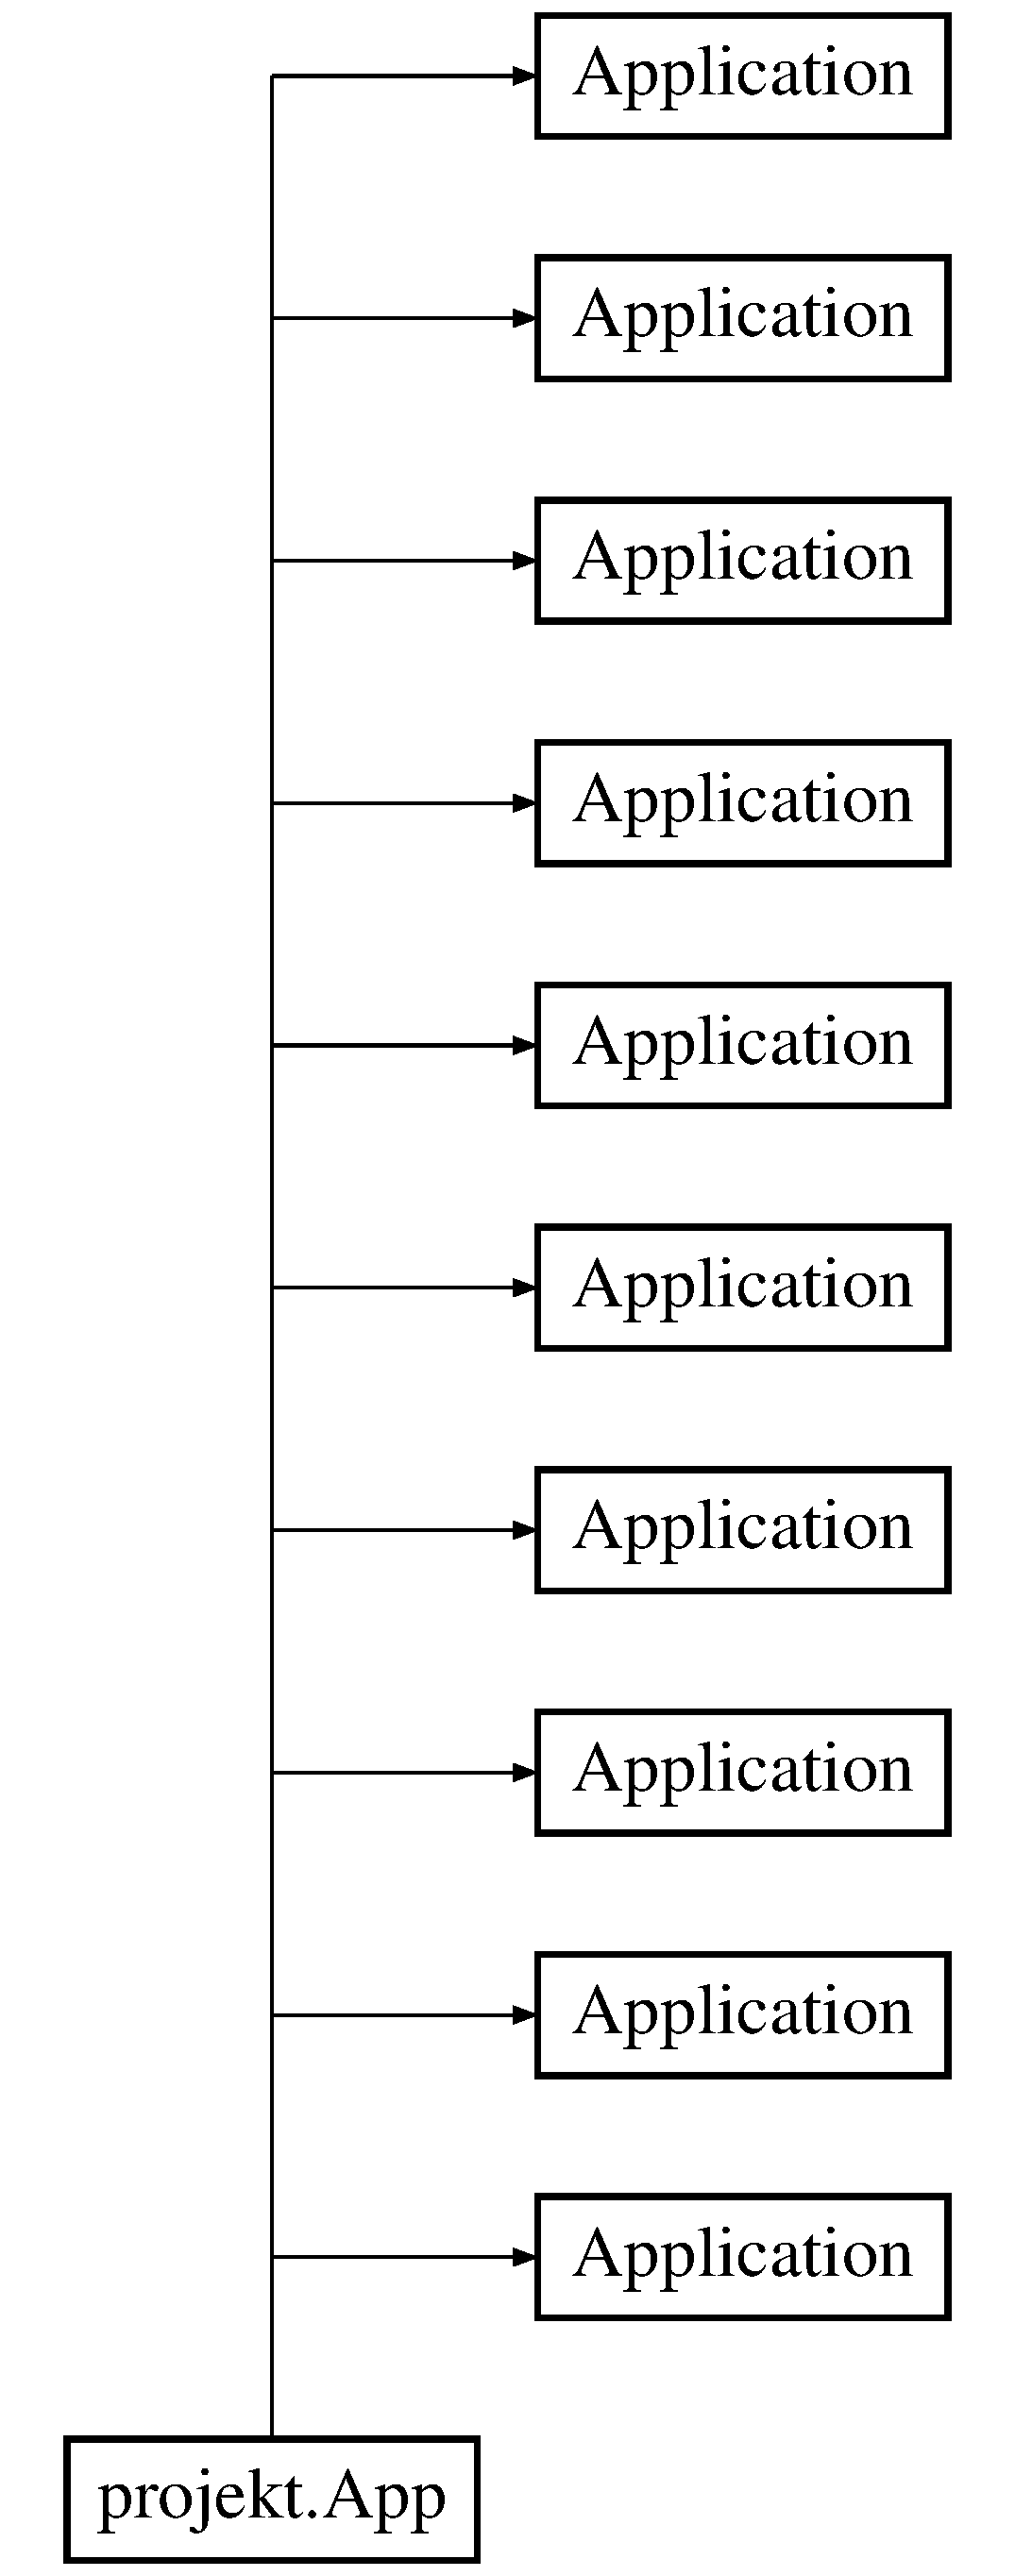
\includegraphics[height=11.000000cm]{classprojekt_1_1_app}
\end{center}
\end{figure}
\subsection*{Public Member Functions}
\begin{DoxyCompactItemize}
\item 
void \mbox{\hyperlink{classprojekt_1_1_app_aadb8f9c97545ff79106a903c12558d38}{Initialize\+Component}} ()
\begin{DoxyCompactList}\small\item\em Initialize\+Component \end{DoxyCompactList}\item 
void \mbox{\hyperlink{classprojekt_1_1_app_aadb8f9c97545ff79106a903c12558d38}{Initialize\+Component}} ()
\begin{DoxyCompactList}\small\item\em Initialize\+Component \end{DoxyCompactList}\item 
void \mbox{\hyperlink{classprojekt_1_1_app_aadb8f9c97545ff79106a903c12558d38}{Initialize\+Component}} ()
\begin{DoxyCompactList}\small\item\em Initialize\+Component \end{DoxyCompactList}\item 
void \mbox{\hyperlink{classprojekt_1_1_app_aadb8f9c97545ff79106a903c12558d38}{Initialize\+Component}} ()
\begin{DoxyCompactList}\small\item\em Initialize\+Component \end{DoxyCompactList}\item 
void \mbox{\hyperlink{classprojekt_1_1_app_aadb8f9c97545ff79106a903c12558d38}{Initialize\+Component}} ()
\begin{DoxyCompactList}\small\item\em Initialize\+Component \end{DoxyCompactList}\item 
void \mbox{\hyperlink{classprojekt_1_1_app_aadb8f9c97545ff79106a903c12558d38}{Initialize\+Component}} ()
\begin{DoxyCompactList}\small\item\em Initialize\+Component \end{DoxyCompactList}\item 
void \mbox{\hyperlink{classprojekt_1_1_app_aadb8f9c97545ff79106a903c12558d38}{Initialize\+Component}} ()
\begin{DoxyCompactList}\small\item\em Initialize\+Component \end{DoxyCompactList}\item 
void \mbox{\hyperlink{classprojekt_1_1_app_aadb8f9c97545ff79106a903c12558d38}{Initialize\+Component}} ()
\begin{DoxyCompactList}\small\item\em Initialize\+Component \end{DoxyCompactList}\item 
void \mbox{\hyperlink{classprojekt_1_1_app_aadb8f9c97545ff79106a903c12558d38}{Initialize\+Component}} ()
\begin{DoxyCompactList}\small\item\em Initialize\+Component \end{DoxyCompactList}\end{DoxyCompactItemize}
\subsection*{Static Public Member Functions}
\begin{DoxyCompactItemize}
\item 
static void \mbox{\hyperlink{classprojekt_1_1_app_aa099f0b6d877e4097ec4cbc0f99826ae}{Main}} ()
\begin{DoxyCompactList}\small\item\em Application Entry Point. \end{DoxyCompactList}\item 
static void \mbox{\hyperlink{classprojekt_1_1_app_aa099f0b6d877e4097ec4cbc0f99826ae}{Main}} ()
\begin{DoxyCompactList}\small\item\em Application Entry Point. \end{DoxyCompactList}\item 
static void \mbox{\hyperlink{classprojekt_1_1_app_aa099f0b6d877e4097ec4cbc0f99826ae}{Main}} ()
\begin{DoxyCompactList}\small\item\em Application Entry Point. \end{DoxyCompactList}\item 
static void \mbox{\hyperlink{classprojekt_1_1_app_aa099f0b6d877e4097ec4cbc0f99826ae}{Main}} ()
\begin{DoxyCompactList}\small\item\em Application Entry Point. \end{DoxyCompactList}\item 
static void \mbox{\hyperlink{classprojekt_1_1_app_aa099f0b6d877e4097ec4cbc0f99826ae}{Main}} ()
\begin{DoxyCompactList}\small\item\em Application Entry Point. \end{DoxyCompactList}\item 
static void \mbox{\hyperlink{classprojekt_1_1_app_aa099f0b6d877e4097ec4cbc0f99826ae}{Main}} ()
\begin{DoxyCompactList}\small\item\em Application Entry Point. \end{DoxyCompactList}\item 
static void \mbox{\hyperlink{classprojekt_1_1_app_aa099f0b6d877e4097ec4cbc0f99826ae}{Main}} ()
\begin{DoxyCompactList}\small\item\em Application Entry Point. \end{DoxyCompactList}\item 
static void \mbox{\hyperlink{classprojekt_1_1_app_aa099f0b6d877e4097ec4cbc0f99826ae}{Main}} ()
\begin{DoxyCompactList}\small\item\em Application Entry Point. \end{DoxyCompactList}\item 
static void \mbox{\hyperlink{classprojekt_1_1_app_aa099f0b6d877e4097ec4cbc0f99826ae}{Main}} ()
\begin{DoxyCompactList}\small\item\em Application Entry Point. \end{DoxyCompactList}\end{DoxyCompactItemize}


\subsection{Detailed Description}
Interaction logic for App.\+xaml 

\mbox{\hyperlink{classprojekt_1_1_app}{App}} 

\subsection{Member Function Documentation}
\mbox{\Hypertarget{classprojekt_1_1_app_aadb8f9c97545ff79106a903c12558d38}\label{classprojekt_1_1_app_aadb8f9c97545ff79106a903c12558d38}} 
\index{projekt\+::\+App@{projekt\+::\+App}!Initialize\+Component@{Initialize\+Component}}
\index{Initialize\+Component@{Initialize\+Component}!projekt\+::\+App@{projekt\+::\+App}}
\subsubsection{\texorpdfstring{Initialize\+Component()}{InitializeComponent()}\hspace{0.1cm}{\footnotesize\ttfamily [1/9]}}
{\footnotesize\ttfamily void projekt.\+App.\+Initialize\+Component (\begin{DoxyParamCaption}{ }\end{DoxyParamCaption})\hspace{0.3cm}{\ttfamily [inline]}}



Initialize\+Component 

\mbox{\Hypertarget{classprojekt_1_1_app_aadb8f9c97545ff79106a903c12558d38}\label{classprojekt_1_1_app_aadb8f9c97545ff79106a903c12558d38}} 
\index{projekt\+::\+App@{projekt\+::\+App}!Initialize\+Component@{Initialize\+Component}}
\index{Initialize\+Component@{Initialize\+Component}!projekt\+::\+App@{projekt\+::\+App}}
\subsubsection{\texorpdfstring{Initialize\+Component()}{InitializeComponent()}\hspace{0.1cm}{\footnotesize\ttfamily [2/9]}}
{\footnotesize\ttfamily void projekt.\+App.\+Initialize\+Component (\begin{DoxyParamCaption}{ }\end{DoxyParamCaption})\hspace{0.3cm}{\ttfamily [inline]}}



Initialize\+Component 

\mbox{\Hypertarget{classprojekt_1_1_app_aadb8f9c97545ff79106a903c12558d38}\label{classprojekt_1_1_app_aadb8f9c97545ff79106a903c12558d38}} 
\index{projekt\+::\+App@{projekt\+::\+App}!Initialize\+Component@{Initialize\+Component}}
\index{Initialize\+Component@{Initialize\+Component}!projekt\+::\+App@{projekt\+::\+App}}
\subsubsection{\texorpdfstring{Initialize\+Component()}{InitializeComponent()}\hspace{0.1cm}{\footnotesize\ttfamily [3/9]}}
{\footnotesize\ttfamily void projekt.\+App.\+Initialize\+Component (\begin{DoxyParamCaption}{ }\end{DoxyParamCaption})\hspace{0.3cm}{\ttfamily [inline]}}



Initialize\+Component 

\mbox{\Hypertarget{classprojekt_1_1_app_aadb8f9c97545ff79106a903c12558d38}\label{classprojekt_1_1_app_aadb8f9c97545ff79106a903c12558d38}} 
\index{projekt\+::\+App@{projekt\+::\+App}!Initialize\+Component@{Initialize\+Component}}
\index{Initialize\+Component@{Initialize\+Component}!projekt\+::\+App@{projekt\+::\+App}}
\subsubsection{\texorpdfstring{Initialize\+Component()}{InitializeComponent()}\hspace{0.1cm}{\footnotesize\ttfamily [4/9]}}
{\footnotesize\ttfamily void projekt.\+App.\+Initialize\+Component (\begin{DoxyParamCaption}{ }\end{DoxyParamCaption})\hspace{0.3cm}{\ttfamily [inline]}}



Initialize\+Component 

\mbox{\Hypertarget{classprojekt_1_1_app_aadb8f9c97545ff79106a903c12558d38}\label{classprojekt_1_1_app_aadb8f9c97545ff79106a903c12558d38}} 
\index{projekt\+::\+App@{projekt\+::\+App}!Initialize\+Component@{Initialize\+Component}}
\index{Initialize\+Component@{Initialize\+Component}!projekt\+::\+App@{projekt\+::\+App}}
\subsubsection{\texorpdfstring{Initialize\+Component()}{InitializeComponent()}\hspace{0.1cm}{\footnotesize\ttfamily [5/9]}}
{\footnotesize\ttfamily void projekt.\+App.\+Initialize\+Component (\begin{DoxyParamCaption}{ }\end{DoxyParamCaption})\hspace{0.3cm}{\ttfamily [inline]}}



Initialize\+Component 

\mbox{\Hypertarget{classprojekt_1_1_app_aadb8f9c97545ff79106a903c12558d38}\label{classprojekt_1_1_app_aadb8f9c97545ff79106a903c12558d38}} 
\index{projekt\+::\+App@{projekt\+::\+App}!Initialize\+Component@{Initialize\+Component}}
\index{Initialize\+Component@{Initialize\+Component}!projekt\+::\+App@{projekt\+::\+App}}
\subsubsection{\texorpdfstring{Initialize\+Component()}{InitializeComponent()}\hspace{0.1cm}{\footnotesize\ttfamily [6/9]}}
{\footnotesize\ttfamily void projekt.\+App.\+Initialize\+Component (\begin{DoxyParamCaption}{ }\end{DoxyParamCaption})\hspace{0.3cm}{\ttfamily [inline]}}



Initialize\+Component 

\mbox{\Hypertarget{classprojekt_1_1_app_aadb8f9c97545ff79106a903c12558d38}\label{classprojekt_1_1_app_aadb8f9c97545ff79106a903c12558d38}} 
\index{projekt\+::\+App@{projekt\+::\+App}!Initialize\+Component@{Initialize\+Component}}
\index{Initialize\+Component@{Initialize\+Component}!projekt\+::\+App@{projekt\+::\+App}}
\subsubsection{\texorpdfstring{Initialize\+Component()}{InitializeComponent()}\hspace{0.1cm}{\footnotesize\ttfamily [7/9]}}
{\footnotesize\ttfamily void projekt.\+App.\+Initialize\+Component (\begin{DoxyParamCaption}{ }\end{DoxyParamCaption})\hspace{0.3cm}{\ttfamily [inline]}}



Initialize\+Component 

\mbox{\Hypertarget{classprojekt_1_1_app_aadb8f9c97545ff79106a903c12558d38}\label{classprojekt_1_1_app_aadb8f9c97545ff79106a903c12558d38}} 
\index{projekt\+::\+App@{projekt\+::\+App}!Initialize\+Component@{Initialize\+Component}}
\index{Initialize\+Component@{Initialize\+Component}!projekt\+::\+App@{projekt\+::\+App}}
\subsubsection{\texorpdfstring{Initialize\+Component()}{InitializeComponent()}\hspace{0.1cm}{\footnotesize\ttfamily [8/9]}}
{\footnotesize\ttfamily void projekt.\+App.\+Initialize\+Component (\begin{DoxyParamCaption}{ }\end{DoxyParamCaption})\hspace{0.3cm}{\ttfamily [inline]}}



Initialize\+Component 

\mbox{\Hypertarget{classprojekt_1_1_app_aadb8f9c97545ff79106a903c12558d38}\label{classprojekt_1_1_app_aadb8f9c97545ff79106a903c12558d38}} 
\index{projekt\+::\+App@{projekt\+::\+App}!Initialize\+Component@{Initialize\+Component}}
\index{Initialize\+Component@{Initialize\+Component}!projekt\+::\+App@{projekt\+::\+App}}
\subsubsection{\texorpdfstring{Initialize\+Component()}{InitializeComponent()}\hspace{0.1cm}{\footnotesize\ttfamily [9/9]}}
{\footnotesize\ttfamily void projekt.\+App.\+Initialize\+Component (\begin{DoxyParamCaption}{ }\end{DoxyParamCaption})\hspace{0.3cm}{\ttfamily [inline]}}



Initialize\+Component 

\mbox{\Hypertarget{classprojekt_1_1_app_aa099f0b6d877e4097ec4cbc0f99826ae}\label{classprojekt_1_1_app_aa099f0b6d877e4097ec4cbc0f99826ae}} 
\index{projekt\+::\+App@{projekt\+::\+App}!Main@{Main}}
\index{Main@{Main}!projekt\+::\+App@{projekt\+::\+App}}
\subsubsection{\texorpdfstring{Main()}{Main()}\hspace{0.1cm}{\footnotesize\ttfamily [1/9]}}
{\footnotesize\ttfamily static void projekt.\+App.\+Main (\begin{DoxyParamCaption}{ }\end{DoxyParamCaption})\hspace{0.3cm}{\ttfamily [inline]}, {\ttfamily [static]}}



Application Entry Point. 

\mbox{\Hypertarget{classprojekt_1_1_app_aa099f0b6d877e4097ec4cbc0f99826ae}\label{classprojekt_1_1_app_aa099f0b6d877e4097ec4cbc0f99826ae}} 
\index{projekt\+::\+App@{projekt\+::\+App}!Main@{Main}}
\index{Main@{Main}!projekt\+::\+App@{projekt\+::\+App}}
\subsubsection{\texorpdfstring{Main()}{Main()}\hspace{0.1cm}{\footnotesize\ttfamily [2/9]}}
{\footnotesize\ttfamily static void projekt.\+App.\+Main (\begin{DoxyParamCaption}{ }\end{DoxyParamCaption})\hspace{0.3cm}{\ttfamily [inline]}, {\ttfamily [static]}}



Application Entry Point. 

\mbox{\Hypertarget{classprojekt_1_1_app_aa099f0b6d877e4097ec4cbc0f99826ae}\label{classprojekt_1_1_app_aa099f0b6d877e4097ec4cbc0f99826ae}} 
\index{projekt\+::\+App@{projekt\+::\+App}!Main@{Main}}
\index{Main@{Main}!projekt\+::\+App@{projekt\+::\+App}}
\subsubsection{\texorpdfstring{Main()}{Main()}\hspace{0.1cm}{\footnotesize\ttfamily [3/9]}}
{\footnotesize\ttfamily static void projekt.\+App.\+Main (\begin{DoxyParamCaption}{ }\end{DoxyParamCaption})\hspace{0.3cm}{\ttfamily [inline]}, {\ttfamily [static]}}



Application Entry Point. 

\mbox{\Hypertarget{classprojekt_1_1_app_aa099f0b6d877e4097ec4cbc0f99826ae}\label{classprojekt_1_1_app_aa099f0b6d877e4097ec4cbc0f99826ae}} 
\index{projekt\+::\+App@{projekt\+::\+App}!Main@{Main}}
\index{Main@{Main}!projekt\+::\+App@{projekt\+::\+App}}
\subsubsection{\texorpdfstring{Main()}{Main()}\hspace{0.1cm}{\footnotesize\ttfamily [4/9]}}
{\footnotesize\ttfamily static void projekt.\+App.\+Main (\begin{DoxyParamCaption}{ }\end{DoxyParamCaption})\hspace{0.3cm}{\ttfamily [inline]}, {\ttfamily [static]}}



Application Entry Point. 

\mbox{\Hypertarget{classprojekt_1_1_app_aa099f0b6d877e4097ec4cbc0f99826ae}\label{classprojekt_1_1_app_aa099f0b6d877e4097ec4cbc0f99826ae}} 
\index{projekt\+::\+App@{projekt\+::\+App}!Main@{Main}}
\index{Main@{Main}!projekt\+::\+App@{projekt\+::\+App}}
\subsubsection{\texorpdfstring{Main()}{Main()}\hspace{0.1cm}{\footnotesize\ttfamily [5/9]}}
{\footnotesize\ttfamily static void projekt.\+App.\+Main (\begin{DoxyParamCaption}{ }\end{DoxyParamCaption})\hspace{0.3cm}{\ttfamily [inline]}, {\ttfamily [static]}}



Application Entry Point. 

\mbox{\Hypertarget{classprojekt_1_1_app_aa099f0b6d877e4097ec4cbc0f99826ae}\label{classprojekt_1_1_app_aa099f0b6d877e4097ec4cbc0f99826ae}} 
\index{projekt\+::\+App@{projekt\+::\+App}!Main@{Main}}
\index{Main@{Main}!projekt\+::\+App@{projekt\+::\+App}}
\subsubsection{\texorpdfstring{Main()}{Main()}\hspace{0.1cm}{\footnotesize\ttfamily [6/9]}}
{\footnotesize\ttfamily static void projekt.\+App.\+Main (\begin{DoxyParamCaption}{ }\end{DoxyParamCaption})\hspace{0.3cm}{\ttfamily [inline]}, {\ttfamily [static]}}



Application Entry Point. 

\mbox{\Hypertarget{classprojekt_1_1_app_aa099f0b6d877e4097ec4cbc0f99826ae}\label{classprojekt_1_1_app_aa099f0b6d877e4097ec4cbc0f99826ae}} 
\index{projekt\+::\+App@{projekt\+::\+App}!Main@{Main}}
\index{Main@{Main}!projekt\+::\+App@{projekt\+::\+App}}
\subsubsection{\texorpdfstring{Main()}{Main()}\hspace{0.1cm}{\footnotesize\ttfamily [7/9]}}
{\footnotesize\ttfamily static void projekt.\+App.\+Main (\begin{DoxyParamCaption}{ }\end{DoxyParamCaption})\hspace{0.3cm}{\ttfamily [inline]}, {\ttfamily [static]}}



Application Entry Point. 

\mbox{\Hypertarget{classprojekt_1_1_app_aa099f0b6d877e4097ec4cbc0f99826ae}\label{classprojekt_1_1_app_aa099f0b6d877e4097ec4cbc0f99826ae}} 
\index{projekt\+::\+App@{projekt\+::\+App}!Main@{Main}}
\index{Main@{Main}!projekt\+::\+App@{projekt\+::\+App}}
\subsubsection{\texorpdfstring{Main()}{Main()}\hspace{0.1cm}{\footnotesize\ttfamily [8/9]}}
{\footnotesize\ttfamily static void projekt.\+App.\+Main (\begin{DoxyParamCaption}{ }\end{DoxyParamCaption})\hspace{0.3cm}{\ttfamily [inline]}, {\ttfamily [static]}}



Application Entry Point. 

\mbox{\Hypertarget{classprojekt_1_1_app_aa099f0b6d877e4097ec4cbc0f99826ae}\label{classprojekt_1_1_app_aa099f0b6d877e4097ec4cbc0f99826ae}} 
\index{projekt\+::\+App@{projekt\+::\+App}!Main@{Main}}
\index{Main@{Main}!projekt\+::\+App@{projekt\+::\+App}}
\subsubsection{\texorpdfstring{Main()}{Main()}\hspace{0.1cm}{\footnotesize\ttfamily [9/9]}}
{\footnotesize\ttfamily static void projekt.\+App.\+Main (\begin{DoxyParamCaption}{ }\end{DoxyParamCaption})\hspace{0.3cm}{\ttfamily [inline]}, {\ttfamily [static]}}



Application Entry Point. 



The documentation for this class was generated from the following files\+:\begin{DoxyCompactItemize}
\item 
projekt/\mbox{\hyperlink{_app_8xaml_8cs}{App.\+xaml.\+cs}}\item 
projekt/obj/\+Debug/\mbox{\hyperlink{_debug_2_app_8g_8cs}{App.\+g.\+cs}}\item 
projekt/obj/\+Debug/\mbox{\hyperlink{_debug_2_app_8g_8i_8cs}{App.\+g.\+i.\+cs}}\end{DoxyCompactItemize}

\hypertarget{classprojekt_1_1_data_set1}{}\section{projekt.\+Data\+Set1 Class Reference}
\label{classprojekt_1_1_data_set1}\index{projekt.\+Data\+Set1@{projekt.\+Data\+Set1}}


Represents a strongly typed in-\/memory cache of data. /summary$>$  


Inheritance diagram for projekt.\+Data\+Set1\+:\begin{figure}[H]
\begin{center}
\leavevmode
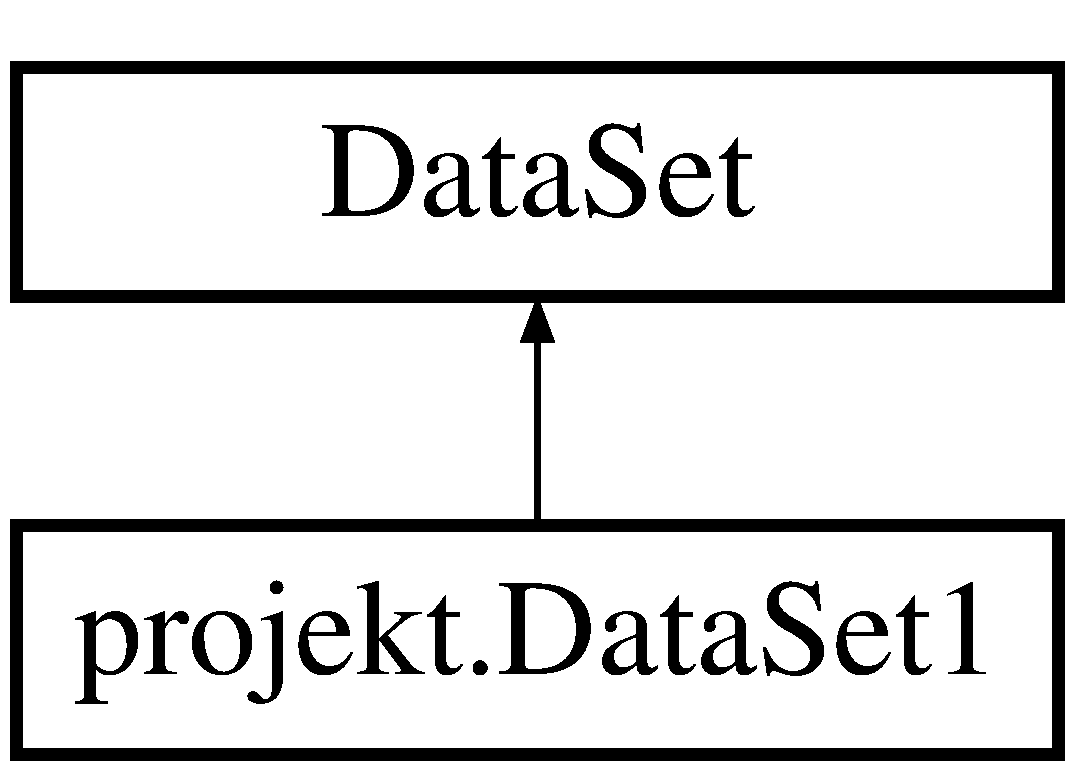
\includegraphics[height=2.000000cm]{classprojekt_1_1_data_set1}
\end{center}
\end{figure}
\subsection*{Public Member Functions}
\begin{DoxyCompactItemize}
\item 
\mbox{\Hypertarget{classprojekt_1_1_data_set1_a26f9dfcb33b30d3fc701574725273fd6}\label{classprojekt_1_1_data_set1_a26f9dfcb33b30d3fc701574725273fd6}} 
override global\+::\+System.\+Data.\+Data\+Set {\bfseries Clone} ()
\end{DoxyCompactItemize}
\subsection*{Static Public Member Functions}
\begin{DoxyCompactItemize}
\item 
\mbox{\Hypertarget{classprojekt_1_1_data_set1_af75a036bac30217b6582f66785499005}\label{classprojekt_1_1_data_set1_af75a036bac30217b6582f66785499005}} 
static global\+::\+System.\+Xml.\+Schema.\+Xml\+Schema\+Complex\+Type {\bfseries Get\+Typed\+Data\+Set\+Schema} (global\+::\+System.\+Xml.\+Schema.\+Xml\+Schema\+Set xs)
\end{DoxyCompactItemize}
\subsection*{Protected Member Functions}
\begin{DoxyCompactItemize}
\item 
\mbox{\Hypertarget{classprojekt_1_1_data_set1_a276b4a5f57cb8de1a39b36dedefe7613}\label{classprojekt_1_1_data_set1_a276b4a5f57cb8de1a39b36dedefe7613}} 
{\bfseries Data\+Set1} (global\+::\+System.\+Runtime.\+Serialization.\+Serialization\+Info info, global\+::\+System.\+Runtime.\+Serialization.\+Streaming\+Context context)
\item 
\mbox{\Hypertarget{classprojekt_1_1_data_set1_a0a252a70e692ec9dc27bfe7371ce3f1b}\label{classprojekt_1_1_data_set1_a0a252a70e692ec9dc27bfe7371ce3f1b}} 
override void {\bfseries Initialize\+Derived\+Data\+Set} ()
\item 
\mbox{\Hypertarget{classprojekt_1_1_data_set1_a3a1de8b5f42f1062608d6c1c683cd5bd}\label{classprojekt_1_1_data_set1_a3a1de8b5f42f1062608d6c1c683cd5bd}} 
override bool {\bfseries Should\+Serialize\+Tables} ()
\item 
\mbox{\Hypertarget{classprojekt_1_1_data_set1_a59de6c98c70128509a6461654eea2766}\label{classprojekt_1_1_data_set1_a59de6c98c70128509a6461654eea2766}} 
override bool {\bfseries Should\+Serialize\+Relations} ()
\item 
\mbox{\Hypertarget{classprojekt_1_1_data_set1_a5a88a43948496bdc4d9ddcafd794d957}\label{classprojekt_1_1_data_set1_a5a88a43948496bdc4d9ddcafd794d957}} 
override void {\bfseries Read\+Xml\+Serializable} (global\+::\+System.\+Xml.\+Xml\+Reader reader)
\item 
\mbox{\Hypertarget{classprojekt_1_1_data_set1_a33a74f619d82064876ccb5caf72a83ff}\label{classprojekt_1_1_data_set1_a33a74f619d82064876ccb5caf72a83ff}} 
override global\+::\+System.\+Xml.\+Schema.\+Xml\+Schema {\bfseries Get\+Schema\+Serializable} ()
\end{DoxyCompactItemize}
\subsection*{Properties}
\begin{DoxyCompactItemize}
\item 
\mbox{\Hypertarget{classprojekt_1_1_data_set1_a427450e2d66c48970331311264026734}\label{classprojekt_1_1_data_set1_a427450e2d66c48970331311264026734}} 
override global\+::\+System.\+Data.\+Schema\+Serialization\+Mode {\bfseries Schema\+Serialization\+Mode}\hspace{0.3cm}{\ttfamily  \mbox{[}get, set\mbox{]}}
\item 
\mbox{\Hypertarget{classprojekt_1_1_data_set1_a1991a0961ae830e41f424a830589a720}\label{classprojekt_1_1_data_set1_a1991a0961ae830e41f424a830589a720}} 
new global\+::\+System.\+Data.\+Data\+Table\+Collection {\bfseries Tables}\hspace{0.3cm}{\ttfamily  \mbox{[}get\mbox{]}}
\item 
\mbox{\Hypertarget{classprojekt_1_1_data_set1_a6b93e786dcf82bd1c416e96311c865e2}\label{classprojekt_1_1_data_set1_a6b93e786dcf82bd1c416e96311c865e2}} 
new global\+::\+System.\+Data.\+Data\+Relation\+Collection {\bfseries Relations}\hspace{0.3cm}{\ttfamily  \mbox{[}get\mbox{]}}
\end{DoxyCompactItemize}


\subsection{Detailed Description}
Represents a strongly typed in-\/memory cache of data. /summary$>$ 

The documentation for this class was generated from the following file\+:\begin{DoxyCompactItemize}
\item 
projekt/Data\+Set1.\+Designer.\+cs\end{DoxyCompactItemize}

\hypertarget{classprojekt_1_1konto}{}\section{projekt.\+konto Class Reference}
\label{classprojekt_1_1konto}\index{projekt.\+konto@{projekt.\+konto}}


konto  


Inheritance diagram for projekt.\+konto\+:\begin{figure}[H]
\begin{center}
\leavevmode
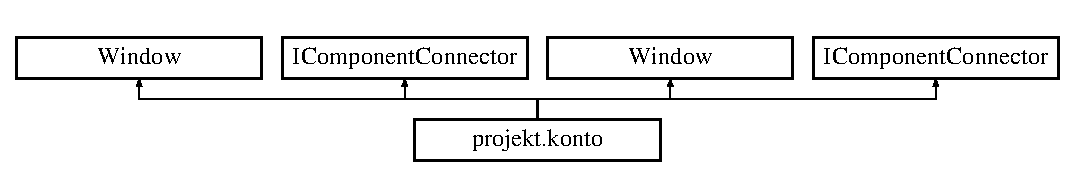
\includegraphics[height=1.931034cm]{classprojekt_1_1konto}
\end{center}
\end{figure}
\subsection*{Public Member Functions}
\begin{DoxyCompactItemize}
\item 
void \mbox{\hyperlink{classprojekt_1_1konto_a7747c72ea9656125d46223a6930f86cf}{Initialize\+Component}} ()
\begin{DoxyCompactList}\small\item\em Initialize\+Component \end{DoxyCompactList}\item 
void \mbox{\hyperlink{classprojekt_1_1konto_a7747c72ea9656125d46223a6930f86cf}{Initialize\+Component}} ()
\begin{DoxyCompactList}\small\item\em Initialize\+Component \end{DoxyCompactList}\end{DoxyCompactItemize}


\subsection{Detailed Description}
konto 



\subsection{Member Function Documentation}
\mbox{\Hypertarget{classprojekt_1_1konto_a7747c72ea9656125d46223a6930f86cf}\label{classprojekt_1_1konto_a7747c72ea9656125d46223a6930f86cf}} 
\index{projekt\+::konto@{projekt\+::konto}!Initialize\+Component@{Initialize\+Component}}
\index{Initialize\+Component@{Initialize\+Component}!projekt\+::konto@{projekt\+::konto}}
\subsubsection{\texorpdfstring{Initialize\+Component()}{InitializeComponent()}\hspace{0.1cm}{\footnotesize\ttfamily [1/2]}}
{\footnotesize\ttfamily void projekt.\+konto.\+Initialize\+Component (\begin{DoxyParamCaption}{ }\end{DoxyParamCaption})\hspace{0.3cm}{\ttfamily [inline]}}



Initialize\+Component 

\mbox{\Hypertarget{classprojekt_1_1konto_a7747c72ea9656125d46223a6930f86cf}\label{classprojekt_1_1konto_a7747c72ea9656125d46223a6930f86cf}} 
\index{projekt\+::konto@{projekt\+::konto}!Initialize\+Component@{Initialize\+Component}}
\index{Initialize\+Component@{Initialize\+Component}!projekt\+::konto@{projekt\+::konto}}
\subsubsection{\texorpdfstring{Initialize\+Component()}{InitializeComponent()}\hspace{0.1cm}{\footnotesize\ttfamily [2/2]}}
{\footnotesize\ttfamily void projekt.\+konto.\+Initialize\+Component (\begin{DoxyParamCaption}{ }\end{DoxyParamCaption})\hspace{0.3cm}{\ttfamily [inline]}}



Initialize\+Component 



The documentation for this class was generated from the following file\+:\begin{DoxyCompactItemize}
\item 
projekt/obj/\+Debug/\mbox{\hyperlink{_debug_2konto_8g_8i_8cs}{konto.\+g.\+i.\+cs}}\end{DoxyCompactItemize}

\hypertarget{classprojekt_1_1konto__u}{}\section{projekt.\+konto\+\_\+u Class Reference}
\label{classprojekt_1_1konto__u}\index{projekt.\+konto\+\_\+u@{projekt.\+konto\+\_\+u}}


konto uzytkownika  


Inheritance diagram for projekt.\+konto\+\_\+u\+:\begin{figure}[H]
\begin{center}
\leavevmode
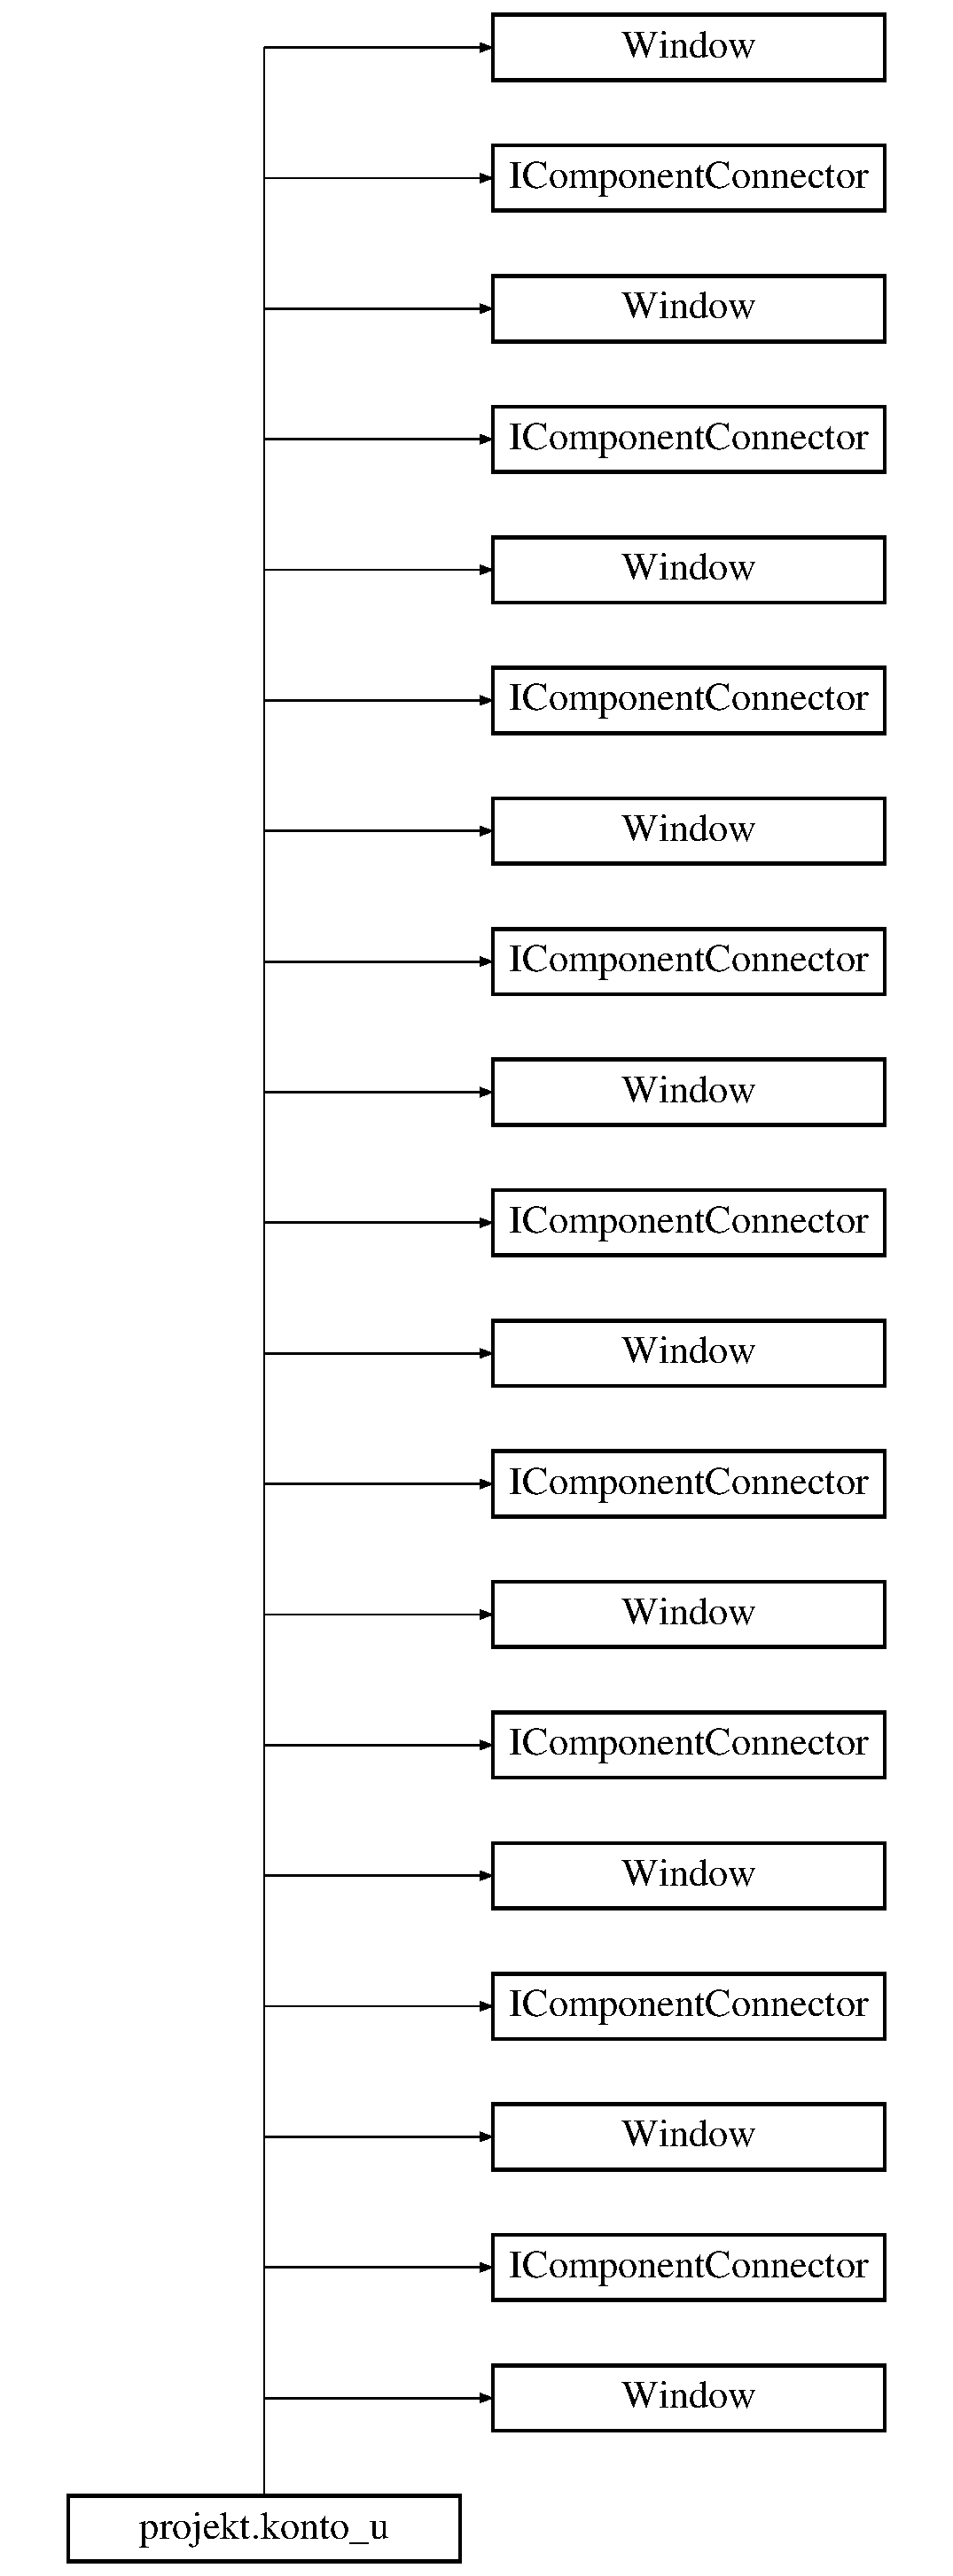
\includegraphics[height=12.000000cm]{classprojekt_1_1konto__u}
\end{center}
\end{figure}
\subsection*{Public Member Functions}
\begin{DoxyCompactItemize}
\item 
\mbox{\hyperlink{classprojekt_1_1konto__u_a3aac4a0ac7618c0eaf58f189236520f5}{konto\+\_\+u}} (string user)
\begin{DoxyCompactList}\small\item\em \mbox{\hyperlink{classprojekt_1_1konto__u}{konto\+\_\+u}} pobranie z bazy nazwy zalogowanego uzytkownika i wyswietlenie. \end{DoxyCompactList}\item 
void \mbox{\hyperlink{classprojekt_1_1konto__u_aba94445ce67074714f9c38935885c165}{Initialize\+Component}} ()
\begin{DoxyCompactList}\small\item\em Initialize\+Component \end{DoxyCompactList}\item 
void \mbox{\hyperlink{classprojekt_1_1konto__u_aba94445ce67074714f9c38935885c165}{Initialize\+Component}} ()
\begin{DoxyCompactList}\small\item\em Initialize\+Component \end{DoxyCompactList}\item 
void \mbox{\hyperlink{classprojekt_1_1konto__u_aba94445ce67074714f9c38935885c165}{Initialize\+Component}} ()
\begin{DoxyCompactList}\small\item\em Initialize\+Component \end{DoxyCompactList}\item 
void \mbox{\hyperlink{classprojekt_1_1konto__u_aba94445ce67074714f9c38935885c165}{Initialize\+Component}} ()
\begin{DoxyCompactList}\small\item\em Initialize\+Component \end{DoxyCompactList}\item 
void \mbox{\hyperlink{classprojekt_1_1konto__u_aba94445ce67074714f9c38935885c165}{Initialize\+Component}} ()
\begin{DoxyCompactList}\small\item\em Initialize\+Component \end{DoxyCompactList}\item 
void \mbox{\hyperlink{classprojekt_1_1konto__u_aba94445ce67074714f9c38935885c165}{Initialize\+Component}} ()
\begin{DoxyCompactList}\small\item\em Initialize\+Component \end{DoxyCompactList}\item 
void \mbox{\hyperlink{classprojekt_1_1konto__u_aba94445ce67074714f9c38935885c165}{Initialize\+Component}} ()
\begin{DoxyCompactList}\small\item\em Initialize\+Component \end{DoxyCompactList}\item 
void \mbox{\hyperlink{classprojekt_1_1konto__u_aba94445ce67074714f9c38935885c165}{Initialize\+Component}} ()
\begin{DoxyCompactList}\small\item\em Initialize\+Component \end{DoxyCompactList}\item 
void \mbox{\hyperlink{classprojekt_1_1konto__u_aba94445ce67074714f9c38935885c165}{Initialize\+Component}} ()
\begin{DoxyCompactList}\small\item\em Initialize\+Component \end{DoxyCompactList}\end{DoxyCompactItemize}


\subsection{Detailed Description}
konto uzytkownika 

\mbox{\hyperlink{classprojekt_1_1konto__u}{konto\+\_\+u}} 

\subsection{Constructor \& Destructor Documentation}
\mbox{\Hypertarget{classprojekt_1_1konto__u_a3aac4a0ac7618c0eaf58f189236520f5}\label{classprojekt_1_1konto__u_a3aac4a0ac7618c0eaf58f189236520f5}} 
\index{projekt\+::konto\+\_\+u@{projekt\+::konto\+\_\+u}!konto\+\_\+u@{konto\+\_\+u}}
\index{konto\+\_\+u@{konto\+\_\+u}!projekt\+::konto\+\_\+u@{projekt\+::konto\+\_\+u}}
\subsubsection{\texorpdfstring{konto\+\_\+u()}{konto\_u()}}
{\footnotesize\ttfamily projekt.\+konto\+\_\+u.\+konto\+\_\+u (\begin{DoxyParamCaption}\item[{string}]{user }\end{DoxyParamCaption})\hspace{0.3cm}{\ttfamily [inline]}}



\mbox{\hyperlink{classprojekt_1_1konto__u}{konto\+\_\+u}} pobranie z bazy nazwy zalogowanego uzytkownika i wyswietlenie. 

po zalogowaniu w panelu logowania w etykiecie zostaje wyświetlona nazwa użytkowanika

\subsection{Member Function Documentation}
\mbox{\Hypertarget{classprojekt_1_1konto__u_aba94445ce67074714f9c38935885c165}\label{classprojekt_1_1konto__u_aba94445ce67074714f9c38935885c165}} 
\index{projekt\+::konto\+\_\+u@{projekt\+::konto\+\_\+u}!Initialize\+Component@{Initialize\+Component}}
\index{Initialize\+Component@{Initialize\+Component}!projekt\+::konto\+\_\+u@{projekt\+::konto\+\_\+u}}
\subsubsection{\texorpdfstring{Initialize\+Component()}{InitializeComponent()}\hspace{0.1cm}{\footnotesize\ttfamily [1/9]}}
{\footnotesize\ttfamily void projekt.\+konto\+\_\+u.\+Initialize\+Component (\begin{DoxyParamCaption}{ }\end{DoxyParamCaption})\hspace{0.3cm}{\ttfamily [inline]}}



Initialize\+Component 

\mbox{\Hypertarget{classprojekt_1_1konto__u_aba94445ce67074714f9c38935885c165}\label{classprojekt_1_1konto__u_aba94445ce67074714f9c38935885c165}} 
\index{projekt\+::konto\+\_\+u@{projekt\+::konto\+\_\+u}!Initialize\+Component@{Initialize\+Component}}
\index{Initialize\+Component@{Initialize\+Component}!projekt\+::konto\+\_\+u@{projekt\+::konto\+\_\+u}}
\subsubsection{\texorpdfstring{Initialize\+Component()}{InitializeComponent()}\hspace{0.1cm}{\footnotesize\ttfamily [2/9]}}
{\footnotesize\ttfamily void projekt.\+konto\+\_\+u.\+Initialize\+Component (\begin{DoxyParamCaption}{ }\end{DoxyParamCaption})\hspace{0.3cm}{\ttfamily [inline]}}



Initialize\+Component 

\mbox{\Hypertarget{classprojekt_1_1konto__u_aba94445ce67074714f9c38935885c165}\label{classprojekt_1_1konto__u_aba94445ce67074714f9c38935885c165}} 
\index{projekt\+::konto\+\_\+u@{projekt\+::konto\+\_\+u}!Initialize\+Component@{Initialize\+Component}}
\index{Initialize\+Component@{Initialize\+Component}!projekt\+::konto\+\_\+u@{projekt\+::konto\+\_\+u}}
\subsubsection{\texorpdfstring{Initialize\+Component()}{InitializeComponent()}\hspace{0.1cm}{\footnotesize\ttfamily [3/9]}}
{\footnotesize\ttfamily void projekt.\+konto\+\_\+u.\+Initialize\+Component (\begin{DoxyParamCaption}{ }\end{DoxyParamCaption})\hspace{0.3cm}{\ttfamily [inline]}}



Initialize\+Component 

\mbox{\Hypertarget{classprojekt_1_1konto__u_aba94445ce67074714f9c38935885c165}\label{classprojekt_1_1konto__u_aba94445ce67074714f9c38935885c165}} 
\index{projekt\+::konto\+\_\+u@{projekt\+::konto\+\_\+u}!Initialize\+Component@{Initialize\+Component}}
\index{Initialize\+Component@{Initialize\+Component}!projekt\+::konto\+\_\+u@{projekt\+::konto\+\_\+u}}
\subsubsection{\texorpdfstring{Initialize\+Component()}{InitializeComponent()}\hspace{0.1cm}{\footnotesize\ttfamily [4/9]}}
{\footnotesize\ttfamily void projekt.\+konto\+\_\+u.\+Initialize\+Component (\begin{DoxyParamCaption}{ }\end{DoxyParamCaption})\hspace{0.3cm}{\ttfamily [inline]}}



Initialize\+Component 

\mbox{\Hypertarget{classprojekt_1_1konto__u_aba94445ce67074714f9c38935885c165}\label{classprojekt_1_1konto__u_aba94445ce67074714f9c38935885c165}} 
\index{projekt\+::konto\+\_\+u@{projekt\+::konto\+\_\+u}!Initialize\+Component@{Initialize\+Component}}
\index{Initialize\+Component@{Initialize\+Component}!projekt\+::konto\+\_\+u@{projekt\+::konto\+\_\+u}}
\subsubsection{\texorpdfstring{Initialize\+Component()}{InitializeComponent()}\hspace{0.1cm}{\footnotesize\ttfamily [5/9]}}
{\footnotesize\ttfamily void projekt.\+konto\+\_\+u.\+Initialize\+Component (\begin{DoxyParamCaption}{ }\end{DoxyParamCaption})\hspace{0.3cm}{\ttfamily [inline]}}



Initialize\+Component 

\mbox{\Hypertarget{classprojekt_1_1konto__u_aba94445ce67074714f9c38935885c165}\label{classprojekt_1_1konto__u_aba94445ce67074714f9c38935885c165}} 
\index{projekt\+::konto\+\_\+u@{projekt\+::konto\+\_\+u}!Initialize\+Component@{Initialize\+Component}}
\index{Initialize\+Component@{Initialize\+Component}!projekt\+::konto\+\_\+u@{projekt\+::konto\+\_\+u}}
\subsubsection{\texorpdfstring{Initialize\+Component()}{InitializeComponent()}\hspace{0.1cm}{\footnotesize\ttfamily [6/9]}}
{\footnotesize\ttfamily void projekt.\+konto\+\_\+u.\+Initialize\+Component (\begin{DoxyParamCaption}{ }\end{DoxyParamCaption})\hspace{0.3cm}{\ttfamily [inline]}}



Initialize\+Component 

\mbox{\Hypertarget{classprojekt_1_1konto__u_aba94445ce67074714f9c38935885c165}\label{classprojekt_1_1konto__u_aba94445ce67074714f9c38935885c165}} 
\index{projekt\+::konto\+\_\+u@{projekt\+::konto\+\_\+u}!Initialize\+Component@{Initialize\+Component}}
\index{Initialize\+Component@{Initialize\+Component}!projekt\+::konto\+\_\+u@{projekt\+::konto\+\_\+u}}
\subsubsection{\texorpdfstring{Initialize\+Component()}{InitializeComponent()}\hspace{0.1cm}{\footnotesize\ttfamily [7/9]}}
{\footnotesize\ttfamily void projekt.\+konto\+\_\+u.\+Initialize\+Component (\begin{DoxyParamCaption}{ }\end{DoxyParamCaption})\hspace{0.3cm}{\ttfamily [inline]}}



Initialize\+Component 

\mbox{\Hypertarget{classprojekt_1_1konto__u_aba94445ce67074714f9c38935885c165}\label{classprojekt_1_1konto__u_aba94445ce67074714f9c38935885c165}} 
\index{projekt\+::konto\+\_\+u@{projekt\+::konto\+\_\+u}!Initialize\+Component@{Initialize\+Component}}
\index{Initialize\+Component@{Initialize\+Component}!projekt\+::konto\+\_\+u@{projekt\+::konto\+\_\+u}}
\subsubsection{\texorpdfstring{Initialize\+Component()}{InitializeComponent()}\hspace{0.1cm}{\footnotesize\ttfamily [8/9]}}
{\footnotesize\ttfamily void projekt.\+konto\+\_\+u.\+Initialize\+Component (\begin{DoxyParamCaption}{ }\end{DoxyParamCaption})\hspace{0.3cm}{\ttfamily [inline]}}



Initialize\+Component 

\mbox{\Hypertarget{classprojekt_1_1konto__u_aba94445ce67074714f9c38935885c165}\label{classprojekt_1_1konto__u_aba94445ce67074714f9c38935885c165}} 
\index{projekt\+::konto\+\_\+u@{projekt\+::konto\+\_\+u}!Initialize\+Component@{Initialize\+Component}}
\index{Initialize\+Component@{Initialize\+Component}!projekt\+::konto\+\_\+u@{projekt\+::konto\+\_\+u}}
\subsubsection{\texorpdfstring{Initialize\+Component()}{InitializeComponent()}\hspace{0.1cm}{\footnotesize\ttfamily [9/9]}}
{\footnotesize\ttfamily void projekt.\+konto\+\_\+u.\+Initialize\+Component (\begin{DoxyParamCaption}{ }\end{DoxyParamCaption})\hspace{0.3cm}{\ttfamily [inline]}}



Initialize\+Component 



The documentation for this class was generated from the following files\+:\begin{DoxyCompactItemize}
\item 
projekt/\mbox{\hyperlink{konto__u_8xaml_8cs}{konto\+\_\+u.\+xaml.\+cs}}\item 
projekt/obj/\+Debug/\mbox{\hyperlink{_debug_2konto__u_8g_8cs}{konto\+\_\+u.\+g.\+cs}}\item 
projekt/obj/\+Debug/\mbox{\hyperlink{_debug_2konto__u_8g_8i_8cs}{konto\+\_\+u.\+g.\+i.\+cs}}\end{DoxyCompactItemize}

\hypertarget{classprojekt_1_1panel1}{}\section{projekt.\+panel1 Class Reference}
\label{classprojekt_1_1panel1}\index{projekt.\+panel1@{projekt.\+panel1}}


\mbox{\hyperlink{classprojekt_1_1panel1}{panel1}}  


Inheritance diagram for projekt.\+panel1\+:\begin{figure}[H]
\begin{center}
\leavevmode
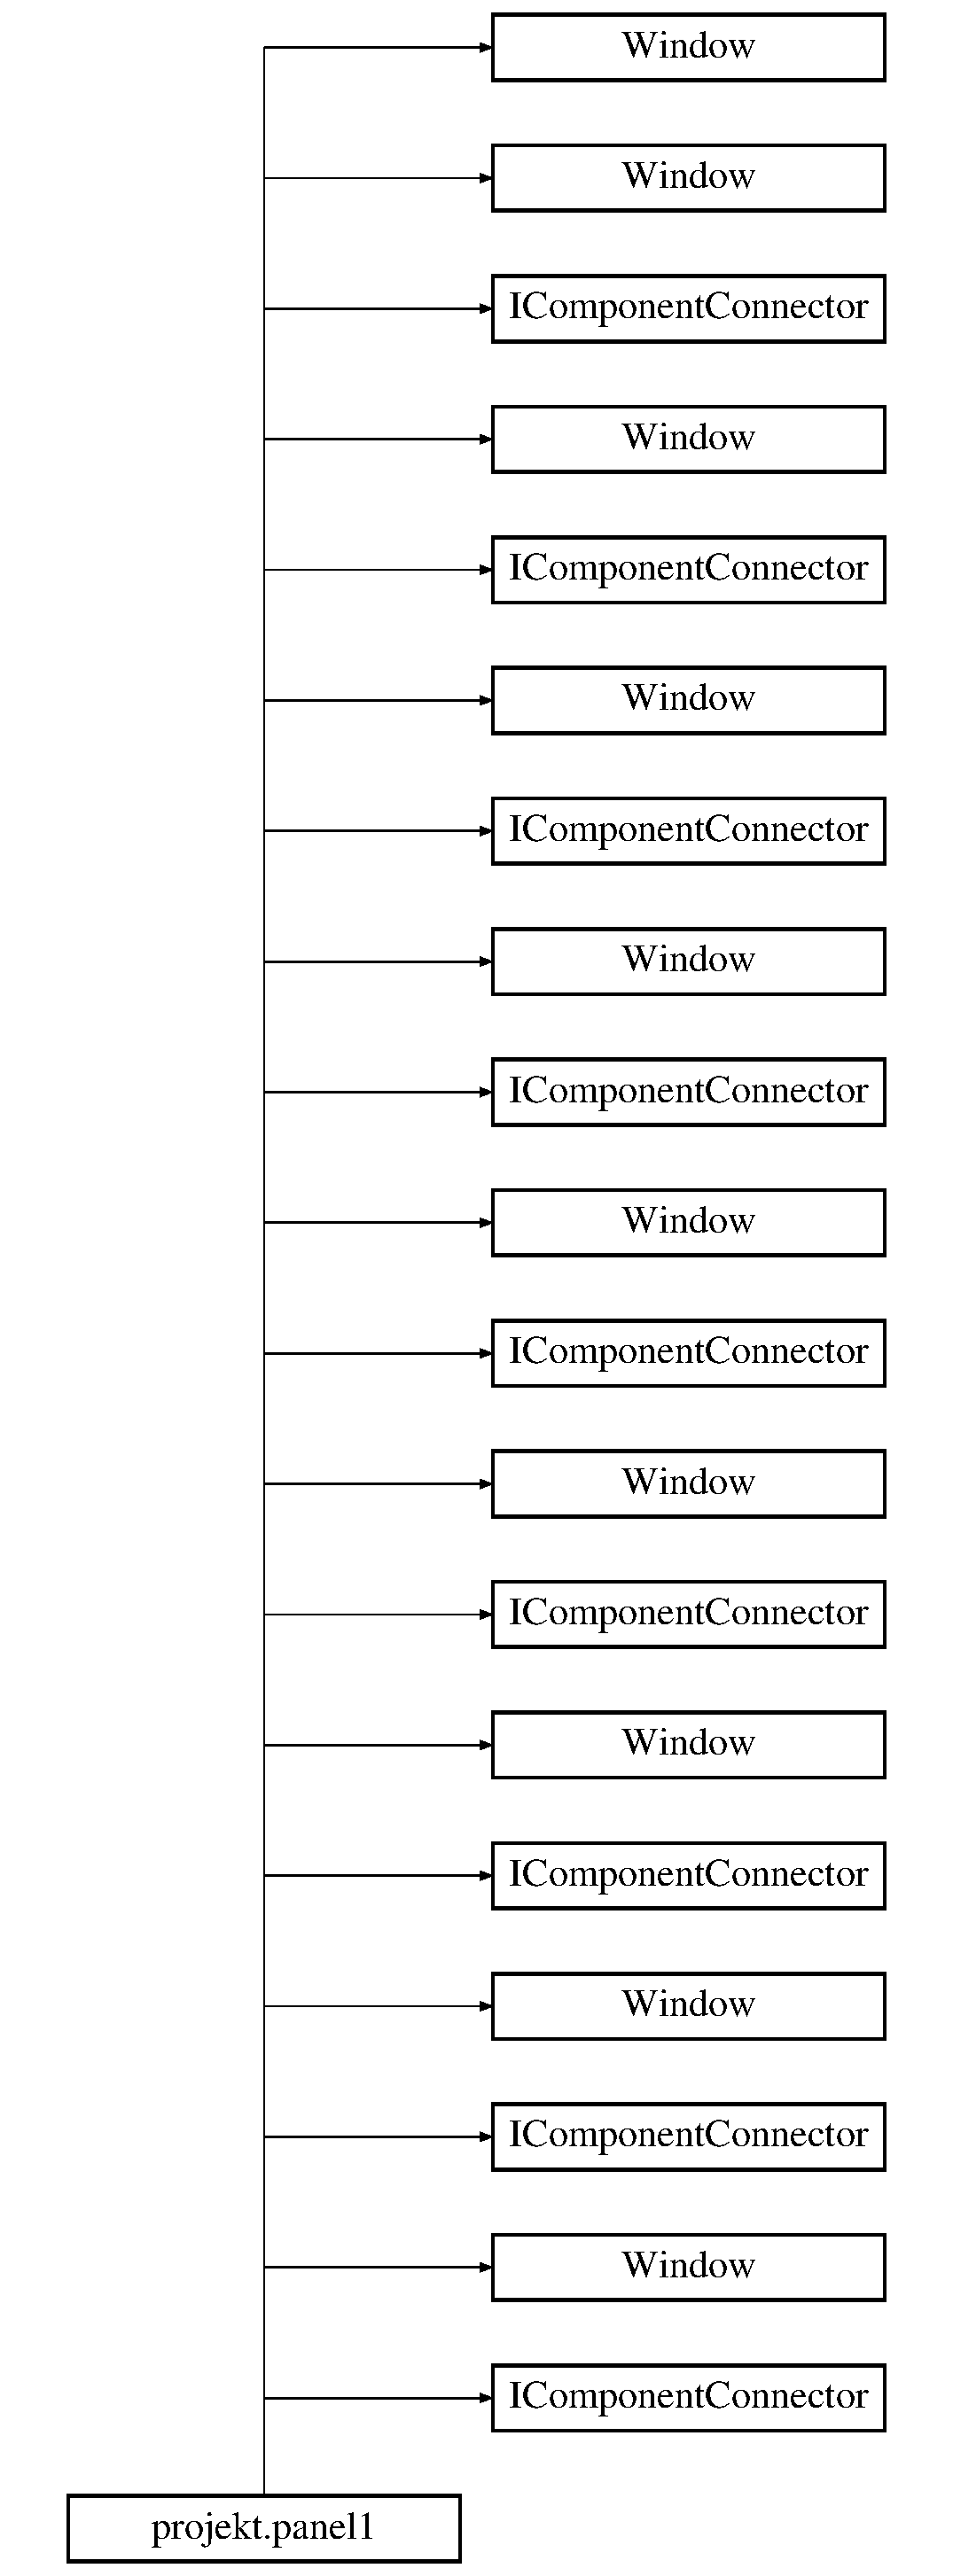
\includegraphics[height=12.000000cm]{classprojekt_1_1panel1}
\end{center}
\end{figure}
\subsection*{Public Member Functions}
\begin{DoxyCompactItemize}
\item 
void \mbox{\hyperlink{classprojekt_1_1panel1_ac484186ff491641f3655f8ae2045bf54}{Initialize\+Component}} ()
\begin{DoxyCompactList}\small\item\em Initialize\+Component \end{DoxyCompactList}\item 
void \mbox{\hyperlink{classprojekt_1_1panel1_ac484186ff491641f3655f8ae2045bf54}{Initialize\+Component}} ()
\begin{DoxyCompactList}\small\item\em Initialize\+Component \end{DoxyCompactList}\item 
void \mbox{\hyperlink{classprojekt_1_1panel1_ac484186ff491641f3655f8ae2045bf54}{Initialize\+Component}} ()
\begin{DoxyCompactList}\small\item\em Initialize\+Component \end{DoxyCompactList}\item 
void \mbox{\hyperlink{classprojekt_1_1panel1_ac484186ff491641f3655f8ae2045bf54}{Initialize\+Component}} ()
\begin{DoxyCompactList}\small\item\em Initialize\+Component \end{DoxyCompactList}\item 
void \mbox{\hyperlink{classprojekt_1_1panel1_ac484186ff491641f3655f8ae2045bf54}{Initialize\+Component}} ()
\begin{DoxyCompactList}\small\item\em Initialize\+Component \end{DoxyCompactList}\item 
void \mbox{\hyperlink{classprojekt_1_1panel1_ac484186ff491641f3655f8ae2045bf54}{Initialize\+Component}} ()
\begin{DoxyCompactList}\small\item\em Initialize\+Component \end{DoxyCompactList}\item 
void \mbox{\hyperlink{classprojekt_1_1panel1_ac484186ff491641f3655f8ae2045bf54}{Initialize\+Component}} ()
\begin{DoxyCompactList}\small\item\em Initialize\+Component \end{DoxyCompactList}\item 
void \mbox{\hyperlink{classprojekt_1_1panel1_ac484186ff491641f3655f8ae2045bf54}{Initialize\+Component}} ()
\begin{DoxyCompactList}\small\item\em Initialize\+Component \end{DoxyCompactList}\item 
void \mbox{\hyperlink{classprojekt_1_1panel1_ac484186ff491641f3655f8ae2045bf54}{Initialize\+Component}} ()
\begin{DoxyCompactList}\small\item\em Initialize\+Component \end{DoxyCompactList}\item 
\mbox{\hyperlink{classprojekt_1_1panel1_a7440a39d8704e252b8d181a930174ef3}{panel1}} ()
\end{DoxyCompactItemize}


\subsection{Detailed Description}
\mbox{\hyperlink{classprojekt_1_1panel1}{panel1}} 

panel początkowy z rejestracją i logowaniem 

\subsection{Constructor \& Destructor Documentation}
\mbox{\Hypertarget{classprojekt_1_1panel1_a7440a39d8704e252b8d181a930174ef3}\label{classprojekt_1_1panel1_a7440a39d8704e252b8d181a930174ef3}} 
\index{projekt\+::panel1@{projekt\+::panel1}!panel1@{panel1}}
\index{panel1@{panel1}!projekt\+::panel1@{projekt\+::panel1}}
\subsubsection{\texorpdfstring{panel1()}{panel1()}}
{\footnotesize\ttfamily projekt.\+panel1.\+panel1 (\begin{DoxyParamCaption}{ }\end{DoxyParamCaption})\hspace{0.3cm}{\ttfamily [inline]}}



\subsection{Member Function Documentation}
\mbox{\Hypertarget{classprojekt_1_1panel1_ac484186ff491641f3655f8ae2045bf54}\label{classprojekt_1_1panel1_ac484186ff491641f3655f8ae2045bf54}} 
\index{projekt\+::panel1@{projekt\+::panel1}!Initialize\+Component@{Initialize\+Component}}
\index{Initialize\+Component@{Initialize\+Component}!projekt\+::panel1@{projekt\+::panel1}}
\subsubsection{\texorpdfstring{Initialize\+Component()}{InitializeComponent()}\hspace{0.1cm}{\footnotesize\ttfamily [1/9]}}
{\footnotesize\ttfamily void projekt.\+panel1.\+Initialize\+Component (\begin{DoxyParamCaption}{ }\end{DoxyParamCaption})\hspace{0.3cm}{\ttfamily [inline]}}



Initialize\+Component 

\mbox{\Hypertarget{classprojekt_1_1panel1_ac484186ff491641f3655f8ae2045bf54}\label{classprojekt_1_1panel1_ac484186ff491641f3655f8ae2045bf54}} 
\index{projekt\+::panel1@{projekt\+::panel1}!Initialize\+Component@{Initialize\+Component}}
\index{Initialize\+Component@{Initialize\+Component}!projekt\+::panel1@{projekt\+::panel1}}
\subsubsection{\texorpdfstring{Initialize\+Component()}{InitializeComponent()}\hspace{0.1cm}{\footnotesize\ttfamily [2/9]}}
{\footnotesize\ttfamily void projekt.\+panel1.\+Initialize\+Component (\begin{DoxyParamCaption}{ }\end{DoxyParamCaption})\hspace{0.3cm}{\ttfamily [inline]}}



Initialize\+Component 

\mbox{\Hypertarget{classprojekt_1_1panel1_ac484186ff491641f3655f8ae2045bf54}\label{classprojekt_1_1panel1_ac484186ff491641f3655f8ae2045bf54}} 
\index{projekt\+::panel1@{projekt\+::panel1}!Initialize\+Component@{Initialize\+Component}}
\index{Initialize\+Component@{Initialize\+Component}!projekt\+::panel1@{projekt\+::panel1}}
\subsubsection{\texorpdfstring{Initialize\+Component()}{InitializeComponent()}\hspace{0.1cm}{\footnotesize\ttfamily [3/9]}}
{\footnotesize\ttfamily void projekt.\+panel1.\+Initialize\+Component (\begin{DoxyParamCaption}{ }\end{DoxyParamCaption})\hspace{0.3cm}{\ttfamily [inline]}}



Initialize\+Component 

\mbox{\Hypertarget{classprojekt_1_1panel1_ac484186ff491641f3655f8ae2045bf54}\label{classprojekt_1_1panel1_ac484186ff491641f3655f8ae2045bf54}} 
\index{projekt\+::panel1@{projekt\+::panel1}!Initialize\+Component@{Initialize\+Component}}
\index{Initialize\+Component@{Initialize\+Component}!projekt\+::panel1@{projekt\+::panel1}}
\subsubsection{\texorpdfstring{Initialize\+Component()}{InitializeComponent()}\hspace{0.1cm}{\footnotesize\ttfamily [4/9]}}
{\footnotesize\ttfamily void projekt.\+panel1.\+Initialize\+Component (\begin{DoxyParamCaption}{ }\end{DoxyParamCaption})\hspace{0.3cm}{\ttfamily [inline]}}



Initialize\+Component 

\mbox{\Hypertarget{classprojekt_1_1panel1_ac484186ff491641f3655f8ae2045bf54}\label{classprojekt_1_1panel1_ac484186ff491641f3655f8ae2045bf54}} 
\index{projekt\+::panel1@{projekt\+::panel1}!Initialize\+Component@{Initialize\+Component}}
\index{Initialize\+Component@{Initialize\+Component}!projekt\+::panel1@{projekt\+::panel1}}
\subsubsection{\texorpdfstring{Initialize\+Component()}{InitializeComponent()}\hspace{0.1cm}{\footnotesize\ttfamily [5/9]}}
{\footnotesize\ttfamily void projekt.\+panel1.\+Initialize\+Component (\begin{DoxyParamCaption}{ }\end{DoxyParamCaption})\hspace{0.3cm}{\ttfamily [inline]}}



Initialize\+Component 

\mbox{\Hypertarget{classprojekt_1_1panel1_ac484186ff491641f3655f8ae2045bf54}\label{classprojekt_1_1panel1_ac484186ff491641f3655f8ae2045bf54}} 
\index{projekt\+::panel1@{projekt\+::panel1}!Initialize\+Component@{Initialize\+Component}}
\index{Initialize\+Component@{Initialize\+Component}!projekt\+::panel1@{projekt\+::panel1}}
\subsubsection{\texorpdfstring{Initialize\+Component()}{InitializeComponent()}\hspace{0.1cm}{\footnotesize\ttfamily [6/9]}}
{\footnotesize\ttfamily void projekt.\+panel1.\+Initialize\+Component (\begin{DoxyParamCaption}{ }\end{DoxyParamCaption})\hspace{0.3cm}{\ttfamily [inline]}}



Initialize\+Component 

\mbox{\Hypertarget{classprojekt_1_1panel1_ac484186ff491641f3655f8ae2045bf54}\label{classprojekt_1_1panel1_ac484186ff491641f3655f8ae2045bf54}} 
\index{projekt\+::panel1@{projekt\+::panel1}!Initialize\+Component@{Initialize\+Component}}
\index{Initialize\+Component@{Initialize\+Component}!projekt\+::panel1@{projekt\+::panel1}}
\subsubsection{\texorpdfstring{Initialize\+Component()}{InitializeComponent()}\hspace{0.1cm}{\footnotesize\ttfamily [7/9]}}
{\footnotesize\ttfamily void projekt.\+panel1.\+Initialize\+Component (\begin{DoxyParamCaption}{ }\end{DoxyParamCaption})\hspace{0.3cm}{\ttfamily [inline]}}



Initialize\+Component 

\mbox{\Hypertarget{classprojekt_1_1panel1_ac484186ff491641f3655f8ae2045bf54}\label{classprojekt_1_1panel1_ac484186ff491641f3655f8ae2045bf54}} 
\index{projekt\+::panel1@{projekt\+::panel1}!Initialize\+Component@{Initialize\+Component}}
\index{Initialize\+Component@{Initialize\+Component}!projekt\+::panel1@{projekt\+::panel1}}
\subsubsection{\texorpdfstring{Initialize\+Component()}{InitializeComponent()}\hspace{0.1cm}{\footnotesize\ttfamily [8/9]}}
{\footnotesize\ttfamily void projekt.\+panel1.\+Initialize\+Component (\begin{DoxyParamCaption}{ }\end{DoxyParamCaption})\hspace{0.3cm}{\ttfamily [inline]}}



Initialize\+Component 

\mbox{\Hypertarget{classprojekt_1_1panel1_ac484186ff491641f3655f8ae2045bf54}\label{classprojekt_1_1panel1_ac484186ff491641f3655f8ae2045bf54}} 
\index{projekt\+::panel1@{projekt\+::panel1}!Initialize\+Component@{Initialize\+Component}}
\index{Initialize\+Component@{Initialize\+Component}!projekt\+::panel1@{projekt\+::panel1}}
\subsubsection{\texorpdfstring{Initialize\+Component()}{InitializeComponent()}\hspace{0.1cm}{\footnotesize\ttfamily [9/9]}}
{\footnotesize\ttfamily void projekt.\+panel1.\+Initialize\+Component (\begin{DoxyParamCaption}{ }\end{DoxyParamCaption})\hspace{0.3cm}{\ttfamily [inline]}}



Initialize\+Component 



The documentation for this class was generated from the following files\+:\begin{DoxyCompactItemize}
\item 
projekt/obj/\+Debug/\mbox{\hyperlink{_debug_2panel1_8g_8cs}{panel1.\+g.\+cs}}\item 
projekt/obj/\+Debug/\mbox{\hyperlink{_debug_2panel1_8g_8i_8cs}{panel1.\+g.\+i.\+cs}}\item 
projekt/\mbox{\hyperlink{panel1_8xaml_8cs}{panel1.\+xaml.\+cs}}\end{DoxyCompactItemize}

\hypertarget{classprojekt_1_1panel__log}{}\section{projekt.\+panel\+\_\+log Class Reference}
\label{classprojekt_1_1panel__log}\index{projekt.\+panel\+\_\+log@{projekt.\+panel\+\_\+log}}


\mbox{\hyperlink{classprojekt_1_1panel__log}{panel\+\_\+log}}  


Inheritance diagram for projekt.\+panel\+\_\+log\+:\begin{figure}[H]
\begin{center}
\leavevmode
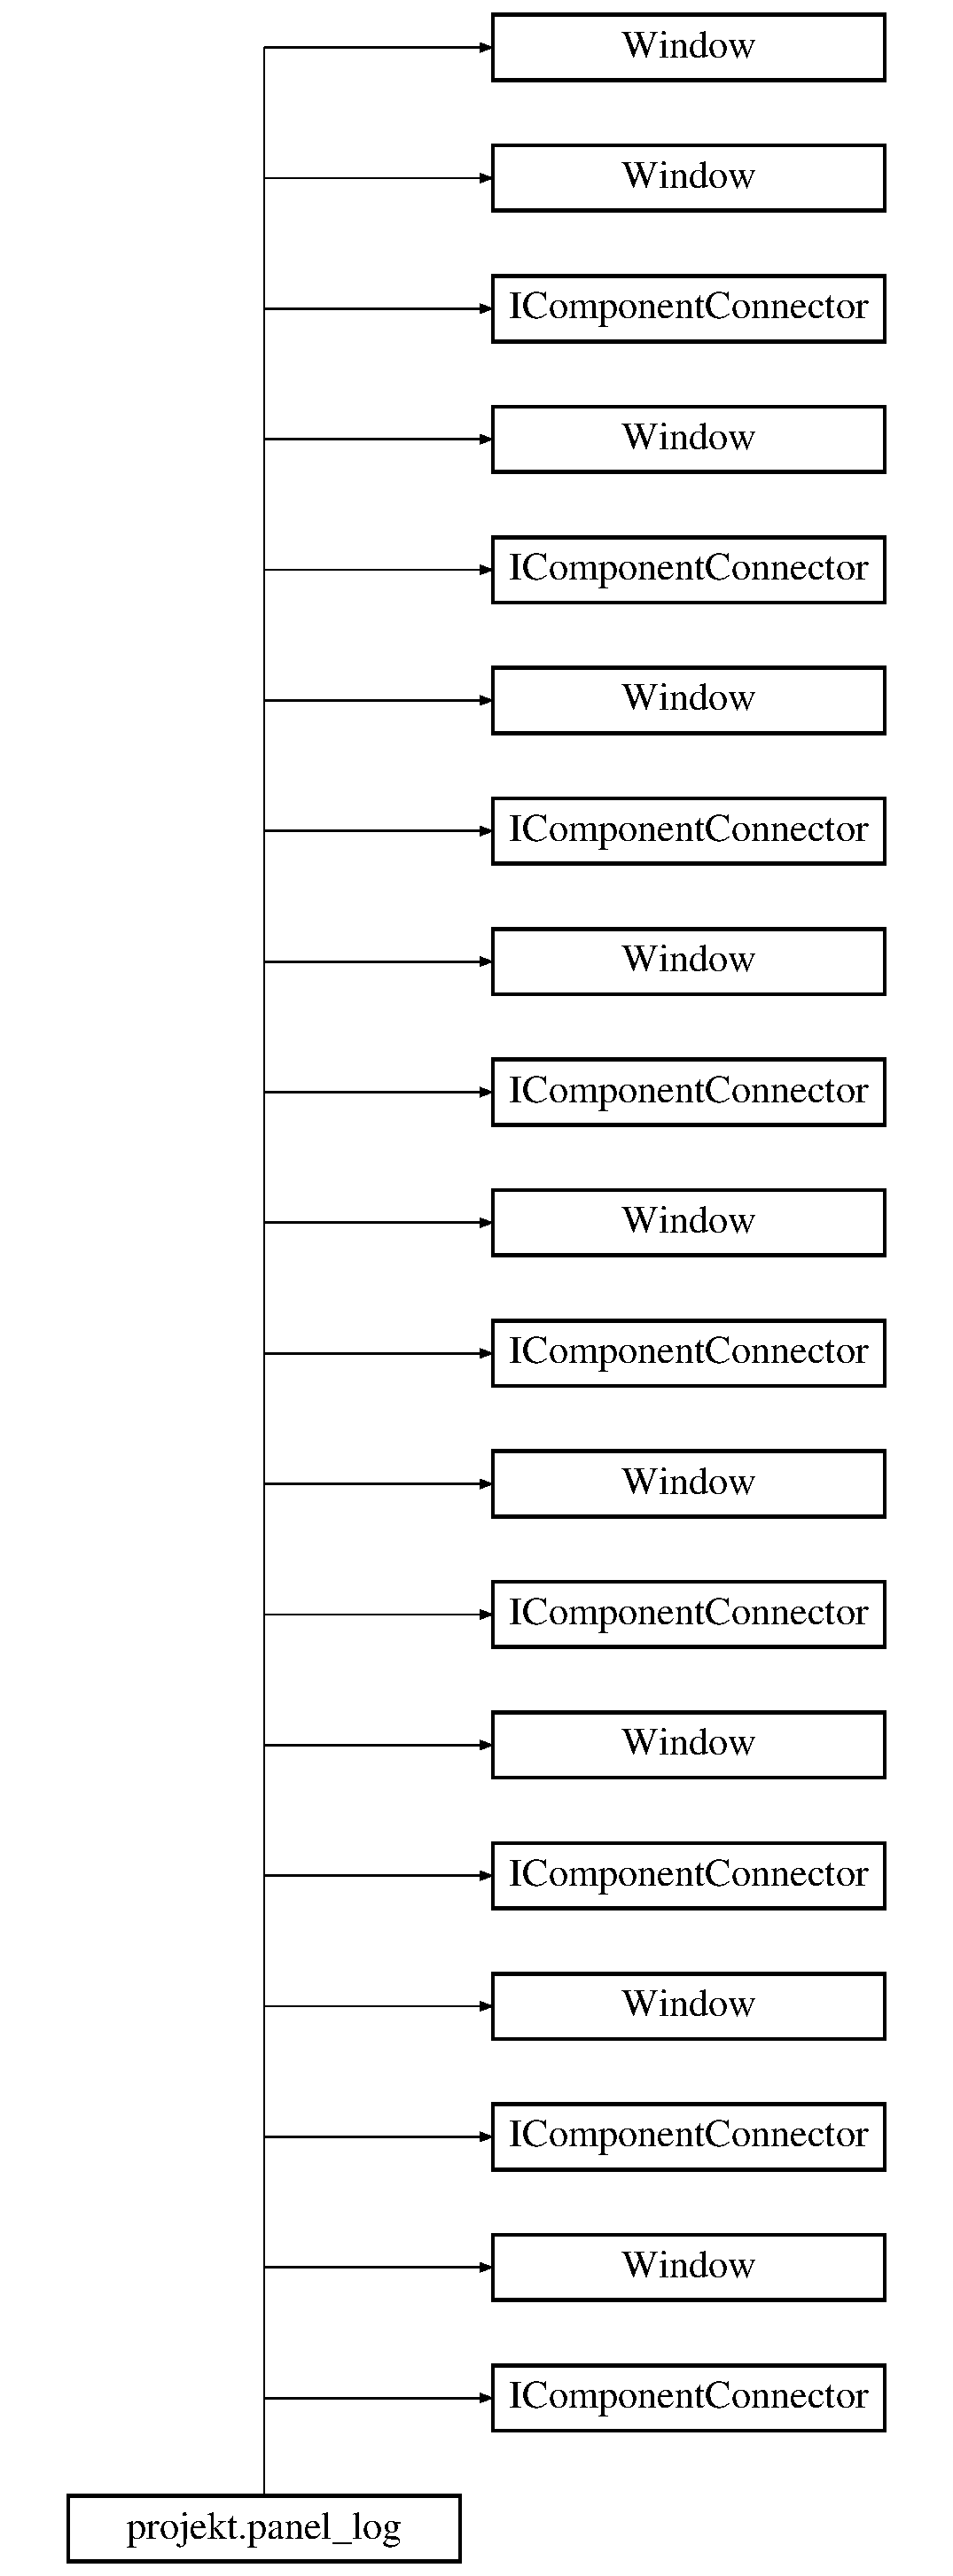
\includegraphics[height=12.000000cm]{classprojekt_1_1panel__log}
\end{center}
\end{figure}
\subsection*{Public Member Functions}
\begin{DoxyCompactItemize}
\item 
void \mbox{\hyperlink{classprojekt_1_1panel__log_a4e106ef7dc0b75cb61bb7018dff7e746}{Initialize\+Component}} ()
\begin{DoxyCompactList}\small\item\em Initialize\+Component \end{DoxyCompactList}\item 
void \mbox{\hyperlink{classprojekt_1_1panel__log_a4e106ef7dc0b75cb61bb7018dff7e746}{Initialize\+Component}} ()
\begin{DoxyCompactList}\small\item\em Initialize\+Component \end{DoxyCompactList}\item 
void \mbox{\hyperlink{classprojekt_1_1panel__log_a4e106ef7dc0b75cb61bb7018dff7e746}{Initialize\+Component}} ()
\begin{DoxyCompactList}\small\item\em Initialize\+Component \end{DoxyCompactList}\item 
void \mbox{\hyperlink{classprojekt_1_1panel__log_a4e106ef7dc0b75cb61bb7018dff7e746}{Initialize\+Component}} ()
\begin{DoxyCompactList}\small\item\em Initialize\+Component \end{DoxyCompactList}\item 
void \mbox{\hyperlink{classprojekt_1_1panel__log_a4e106ef7dc0b75cb61bb7018dff7e746}{Initialize\+Component}} ()
\begin{DoxyCompactList}\small\item\em Initialize\+Component \end{DoxyCompactList}\item 
void \mbox{\hyperlink{classprojekt_1_1panel__log_a4e106ef7dc0b75cb61bb7018dff7e746}{Initialize\+Component}} ()
\begin{DoxyCompactList}\small\item\em Initialize\+Component \end{DoxyCompactList}\item 
void \mbox{\hyperlink{classprojekt_1_1panel__log_a4e106ef7dc0b75cb61bb7018dff7e746}{Initialize\+Component}} ()
\begin{DoxyCompactList}\small\item\em Initialize\+Component \end{DoxyCompactList}\item 
void \mbox{\hyperlink{classprojekt_1_1panel__log_a4e106ef7dc0b75cb61bb7018dff7e746}{Initialize\+Component}} ()
\begin{DoxyCompactList}\small\item\em Initialize\+Component \end{DoxyCompactList}\item 
void \mbox{\hyperlink{classprojekt_1_1panel__log_a4e106ef7dc0b75cb61bb7018dff7e746}{Initialize\+Component}} ()
\begin{DoxyCompactList}\small\item\em Initialize\+Component \end{DoxyCompactList}\item 
\mbox{\hyperlink{classprojekt_1_1panel__log_a96570278e031a563b59923c0acacae9b}{panel\+\_\+log}} ()
\begin{DoxyCompactList}\small\item\em zaczytanie z jakiej ścieżki \mbox{\hyperlink{classprojekt_1_1panel__log}{panel\+\_\+log}} ma zaczytywać bazę danych \end{DoxyCompactList}\item 
void \mbox{\hyperlink{classprojekt_1_1panel__log_ac071ade9d2f740ce0513d72399bf6847}{b\+\_\+zaloguj\+\_\+\+Click}} (object sender, Routed\+Event\+Args e)
\begin{DoxyCompactList}\small\item\em metoda służąca do weryfikowania danych podczas logowania do bazy funkcja przy pomocy pętli weryfikuje po kolei rekordy w bazie, jesli natrafi na taki sam login i hasło wpisane przez uzytkownika nastepuje logowanie, jesli nie zwraca komunikat o błędzie \end{DoxyCompactList}\end{DoxyCompactItemize}


\subsection{Detailed Description}
\mbox{\hyperlink{classprojekt_1_1panel__log}{panel\+\_\+log}} 

panel logowania 

\subsection{Constructor \& Destructor Documentation}
\mbox{\Hypertarget{classprojekt_1_1panel__log_a96570278e031a563b59923c0acacae9b}\label{classprojekt_1_1panel__log_a96570278e031a563b59923c0acacae9b}} 
\index{projekt\+::panel\+\_\+log@{projekt\+::panel\+\_\+log}!panel\+\_\+log@{panel\+\_\+log}}
\index{panel\+\_\+log@{panel\+\_\+log}!projekt\+::panel\+\_\+log@{projekt\+::panel\+\_\+log}}
\subsubsection{\texorpdfstring{panel\+\_\+log()}{panel\_log()}}
{\footnotesize\ttfamily projekt.\+panel\+\_\+log.\+panel\+\_\+log (\begin{DoxyParamCaption}{ }\end{DoxyParamCaption})\hspace{0.3cm}{\ttfamily [inline]}}



zaczytanie z jakiej ścieżki \mbox{\hyperlink{classprojekt_1_1panel__log}{panel\+\_\+log}} ma zaczytywać bazę danych 



\subsection{Member Function Documentation}
\mbox{\Hypertarget{classprojekt_1_1panel__log_ac071ade9d2f740ce0513d72399bf6847}\label{classprojekt_1_1panel__log_ac071ade9d2f740ce0513d72399bf6847}} 
\index{projekt\+::panel\+\_\+log@{projekt\+::panel\+\_\+log}!b\+\_\+zaloguj\+\_\+\+Click@{b\+\_\+zaloguj\+\_\+\+Click}}
\index{b\+\_\+zaloguj\+\_\+\+Click@{b\+\_\+zaloguj\+\_\+\+Click}!projekt\+::panel\+\_\+log@{projekt\+::panel\+\_\+log}}
\subsubsection{\texorpdfstring{b\+\_\+zaloguj\+\_\+\+Click()}{b\_zaloguj\_Click()}}
{\footnotesize\ttfamily void projekt.\+panel\+\_\+log.\+b\+\_\+zaloguj\+\_\+\+Click (\begin{DoxyParamCaption}\item[{object}]{sender,  }\item[{Routed\+Event\+Args}]{e }\end{DoxyParamCaption})\hspace{0.3cm}{\ttfamily [inline]}}



metoda służąca do weryfikowania danych podczas logowania do bazy funkcja przy pomocy pętli weryfikuje po kolei rekordy w bazie, jesli natrafi na taki sam login i hasło wpisane przez uzytkownika nastepuje logowanie, jesli nie zwraca komunikat o błędzie 

metoda zaloguj po kliknięciu while (reader.\+Read()) przy pomocy pętli while zwiększam wartość zmiennej count o 1(będzie to odzwierciedleniem indeksów w bazie, dzięki temu weryfikuje po kolei loginy i hasła wpisane do bazy); ///

count++;

instrukcja if(jesli hasło jest poprawne i się pokrywa 1\+:1 to logowanie następuje i pojawia się komunikat. ~\newline
~\newline
~\newline
~\newline
~\newline
~\newline
~\newline
~\newline
~\newline
~\newline
~\newline
 komuikat

connection.\+Close zamyka połączenie z bazą danych po spełnieniu warunku

baza dysponuje już takimi danymi, dlatego następuje logowanie

zamyka okno

zaczytywanie i przypisywanie loginu do okna Konto uzytkownika

pokaż okno

zamknięcie odczytywania bazy danych

else czyli pozostałe przypadki, jeśli użytkownik wpisze niepoprawne wartości do textboxa loginu lub hasła wyrzuci komunikat o niepoprawnych danych

komunikat

zakmnięcie połączenia z bazą danych

zamknięcie odczytywania danych z bazy \mbox{\Hypertarget{classprojekt_1_1panel__log_a4e106ef7dc0b75cb61bb7018dff7e746}\label{classprojekt_1_1panel__log_a4e106ef7dc0b75cb61bb7018dff7e746}} 
\index{projekt\+::panel\+\_\+log@{projekt\+::panel\+\_\+log}!Initialize\+Component@{Initialize\+Component}}
\index{Initialize\+Component@{Initialize\+Component}!projekt\+::panel\+\_\+log@{projekt\+::panel\+\_\+log}}
\subsubsection{\texorpdfstring{Initialize\+Component()}{InitializeComponent()}\hspace{0.1cm}{\footnotesize\ttfamily [1/9]}}
{\footnotesize\ttfamily void projekt.\+panel\+\_\+log.\+Initialize\+Component (\begin{DoxyParamCaption}{ }\end{DoxyParamCaption})\hspace{0.3cm}{\ttfamily [inline]}}



Initialize\+Component 

\mbox{\Hypertarget{classprojekt_1_1panel__log_a4e106ef7dc0b75cb61bb7018dff7e746}\label{classprojekt_1_1panel__log_a4e106ef7dc0b75cb61bb7018dff7e746}} 
\index{projekt\+::panel\+\_\+log@{projekt\+::panel\+\_\+log}!Initialize\+Component@{Initialize\+Component}}
\index{Initialize\+Component@{Initialize\+Component}!projekt\+::panel\+\_\+log@{projekt\+::panel\+\_\+log}}
\subsubsection{\texorpdfstring{Initialize\+Component()}{InitializeComponent()}\hspace{0.1cm}{\footnotesize\ttfamily [2/9]}}
{\footnotesize\ttfamily void projekt.\+panel\+\_\+log.\+Initialize\+Component (\begin{DoxyParamCaption}{ }\end{DoxyParamCaption})\hspace{0.3cm}{\ttfamily [inline]}}



Initialize\+Component 

\mbox{\Hypertarget{classprojekt_1_1panel__log_a4e106ef7dc0b75cb61bb7018dff7e746}\label{classprojekt_1_1panel__log_a4e106ef7dc0b75cb61bb7018dff7e746}} 
\index{projekt\+::panel\+\_\+log@{projekt\+::panel\+\_\+log}!Initialize\+Component@{Initialize\+Component}}
\index{Initialize\+Component@{Initialize\+Component}!projekt\+::panel\+\_\+log@{projekt\+::panel\+\_\+log}}
\subsubsection{\texorpdfstring{Initialize\+Component()}{InitializeComponent()}\hspace{0.1cm}{\footnotesize\ttfamily [3/9]}}
{\footnotesize\ttfamily void projekt.\+panel\+\_\+log.\+Initialize\+Component (\begin{DoxyParamCaption}{ }\end{DoxyParamCaption})\hspace{0.3cm}{\ttfamily [inline]}}



Initialize\+Component 

\mbox{\Hypertarget{classprojekt_1_1panel__log_a4e106ef7dc0b75cb61bb7018dff7e746}\label{classprojekt_1_1panel__log_a4e106ef7dc0b75cb61bb7018dff7e746}} 
\index{projekt\+::panel\+\_\+log@{projekt\+::panel\+\_\+log}!Initialize\+Component@{Initialize\+Component}}
\index{Initialize\+Component@{Initialize\+Component}!projekt\+::panel\+\_\+log@{projekt\+::panel\+\_\+log}}
\subsubsection{\texorpdfstring{Initialize\+Component()}{InitializeComponent()}\hspace{0.1cm}{\footnotesize\ttfamily [4/9]}}
{\footnotesize\ttfamily void projekt.\+panel\+\_\+log.\+Initialize\+Component (\begin{DoxyParamCaption}{ }\end{DoxyParamCaption})\hspace{0.3cm}{\ttfamily [inline]}}



Initialize\+Component 

\mbox{\Hypertarget{classprojekt_1_1panel__log_a4e106ef7dc0b75cb61bb7018dff7e746}\label{classprojekt_1_1panel__log_a4e106ef7dc0b75cb61bb7018dff7e746}} 
\index{projekt\+::panel\+\_\+log@{projekt\+::panel\+\_\+log}!Initialize\+Component@{Initialize\+Component}}
\index{Initialize\+Component@{Initialize\+Component}!projekt\+::panel\+\_\+log@{projekt\+::panel\+\_\+log}}
\subsubsection{\texorpdfstring{Initialize\+Component()}{InitializeComponent()}\hspace{0.1cm}{\footnotesize\ttfamily [5/9]}}
{\footnotesize\ttfamily void projekt.\+panel\+\_\+log.\+Initialize\+Component (\begin{DoxyParamCaption}{ }\end{DoxyParamCaption})\hspace{0.3cm}{\ttfamily [inline]}}



Initialize\+Component 

\mbox{\Hypertarget{classprojekt_1_1panel__log_a4e106ef7dc0b75cb61bb7018dff7e746}\label{classprojekt_1_1panel__log_a4e106ef7dc0b75cb61bb7018dff7e746}} 
\index{projekt\+::panel\+\_\+log@{projekt\+::panel\+\_\+log}!Initialize\+Component@{Initialize\+Component}}
\index{Initialize\+Component@{Initialize\+Component}!projekt\+::panel\+\_\+log@{projekt\+::panel\+\_\+log}}
\subsubsection{\texorpdfstring{Initialize\+Component()}{InitializeComponent()}\hspace{0.1cm}{\footnotesize\ttfamily [6/9]}}
{\footnotesize\ttfamily void projekt.\+panel\+\_\+log.\+Initialize\+Component (\begin{DoxyParamCaption}{ }\end{DoxyParamCaption})\hspace{0.3cm}{\ttfamily [inline]}}



Initialize\+Component 

\mbox{\Hypertarget{classprojekt_1_1panel__log_a4e106ef7dc0b75cb61bb7018dff7e746}\label{classprojekt_1_1panel__log_a4e106ef7dc0b75cb61bb7018dff7e746}} 
\index{projekt\+::panel\+\_\+log@{projekt\+::panel\+\_\+log}!Initialize\+Component@{Initialize\+Component}}
\index{Initialize\+Component@{Initialize\+Component}!projekt\+::panel\+\_\+log@{projekt\+::panel\+\_\+log}}
\subsubsection{\texorpdfstring{Initialize\+Component()}{InitializeComponent()}\hspace{0.1cm}{\footnotesize\ttfamily [7/9]}}
{\footnotesize\ttfamily void projekt.\+panel\+\_\+log.\+Initialize\+Component (\begin{DoxyParamCaption}{ }\end{DoxyParamCaption})\hspace{0.3cm}{\ttfamily [inline]}}



Initialize\+Component 

\mbox{\Hypertarget{classprojekt_1_1panel__log_a4e106ef7dc0b75cb61bb7018dff7e746}\label{classprojekt_1_1panel__log_a4e106ef7dc0b75cb61bb7018dff7e746}} 
\index{projekt\+::panel\+\_\+log@{projekt\+::panel\+\_\+log}!Initialize\+Component@{Initialize\+Component}}
\index{Initialize\+Component@{Initialize\+Component}!projekt\+::panel\+\_\+log@{projekt\+::panel\+\_\+log}}
\subsubsection{\texorpdfstring{Initialize\+Component()}{InitializeComponent()}\hspace{0.1cm}{\footnotesize\ttfamily [8/9]}}
{\footnotesize\ttfamily void projekt.\+panel\+\_\+log.\+Initialize\+Component (\begin{DoxyParamCaption}{ }\end{DoxyParamCaption})\hspace{0.3cm}{\ttfamily [inline]}}



Initialize\+Component 

\mbox{\Hypertarget{classprojekt_1_1panel__log_a4e106ef7dc0b75cb61bb7018dff7e746}\label{classprojekt_1_1panel__log_a4e106ef7dc0b75cb61bb7018dff7e746}} 
\index{projekt\+::panel\+\_\+log@{projekt\+::panel\+\_\+log}!Initialize\+Component@{Initialize\+Component}}
\index{Initialize\+Component@{Initialize\+Component}!projekt\+::panel\+\_\+log@{projekt\+::panel\+\_\+log}}
\subsubsection{\texorpdfstring{Initialize\+Component()}{InitializeComponent()}\hspace{0.1cm}{\footnotesize\ttfamily [9/9]}}
{\footnotesize\ttfamily void projekt.\+panel\+\_\+log.\+Initialize\+Component (\begin{DoxyParamCaption}{ }\end{DoxyParamCaption})\hspace{0.3cm}{\ttfamily [inline]}}



Initialize\+Component 



The documentation for this class was generated from the following files\+:\begin{DoxyCompactItemize}
\item 
projekt/obj/\+Debug/\mbox{\hyperlink{_debug_2panel__log_8g_8cs}{panel\+\_\+log.\+g.\+cs}}\item 
projekt/obj/\+Debug/\mbox{\hyperlink{_debug_2panel__log_8g_8i_8cs}{panel\+\_\+log.\+g.\+i.\+cs}}\item 
projekt/\mbox{\hyperlink{panel__log_8xaml_8cs}{panel\+\_\+log.\+xaml.\+cs}}\end{DoxyCompactItemize}

\hypertarget{classprojekt_1_1_tests_1_1panel__log_tests}{}\section{projekt.\+Tests.\+panel\+\_\+log\+Tests Class Reference}
\label{classprojekt_1_1_tests_1_1panel__log_tests}\index{projekt.\+Tests.\+panel\+\_\+log\+Tests@{projekt.\+Tests.\+panel\+\_\+log\+Tests}}


 


\subsection*{Public Member Functions}
\begin{DoxyCompactItemize}
\item 
void \mbox{\hyperlink{classprojekt_1_1_tests_1_1panel__log_tests_a0c6089b447469ddabdd5eda42f9e163b}{Test\+Logowania}} ()
\begin{DoxyCompactList}\small\item\em metoda testująca logowanie użytkownika -\/ czy połączenie z bazą i wyszukiwanie w niej działą poprawnie, osiągnięte to zostało poprzez pętle, która sprawdza po kolei każdy wiersz w bazie i weryfikuje czy takie dane występują w tabeli \end{DoxyCompactList}\end{DoxyCompactItemize}


\subsection{Detailed Description}


klasa testująca \mbox{\hyperlink{classprojekt_1_1_tests_1_1panel__log_tests}{panel\+\_\+log\+Tests}} 

\subsection{Member Function Documentation}
\mbox{\Hypertarget{classprojekt_1_1_tests_1_1panel__log_tests_a0c6089b447469ddabdd5eda42f9e163b}\label{classprojekt_1_1_tests_1_1panel__log_tests_a0c6089b447469ddabdd5eda42f9e163b}} 
\index{projekt\+::\+Tests\+::panel\+\_\+log\+Tests@{projekt\+::\+Tests\+::panel\+\_\+log\+Tests}!Test\+Logowania@{Test\+Logowania}}
\index{Test\+Logowania@{Test\+Logowania}!projekt\+::\+Tests\+::panel\+\_\+log\+Tests@{projekt\+::\+Tests\+::panel\+\_\+log\+Tests}}
\subsubsection{\texorpdfstring{Test\+Logowania()}{TestLogowania()}}
{\footnotesize\ttfamily void projekt.\+Tests.\+panel\+\_\+log\+Tests.\+Test\+Logowania (\begin{DoxyParamCaption}{ }\end{DoxyParamCaption})\hspace{0.3cm}{\ttfamily [inline]}}



metoda testująca logowanie użytkownika -\/ czy połączenie z bazą i wyszukiwanie w niej działą poprawnie, osiągnięte to zostało poprzez pętle, która sprawdza po kolei każdy wiersz w bazie i weryfikuje czy takie dane występują w tabeli 

while (reader.\+Read()) przy pomocy pętli while zwiększam wartość zmiennej count o 1(będzie to odzwierciedleniem indeksów w bazie, dzięki temu weryfikuje po kolei loginy i hasła wpisane do bazy); ///

count++;

instrukcja if(jesli hasło jest poprawne i się pokrywa 1\+:1 to logowanie następuje i pojawia się komunikat. ~\newline
~\newline
~\newline
 else czyli pozostałe przypadki, jeśli użytkownik wpisze niepoprawne wartości do textboxa loginu lub hasła wyrzuci komunikat o niepoprawnych danych

zakmnięcie połączenia z bazą danych

zamknięcie odczytywania danych z bazy 

The documentation for this class was generated from the following file\+:\begin{DoxyCompactItemize}
\item 
projekt\+Tests2/\mbox{\hyperlink{panel__log_tests_8cs}{panel\+\_\+log\+Tests.\+cs}}\end{DoxyCompactItemize}

\hypertarget{classprojekt_1_1panel__rej}{}\section{projekt.\+panel\+\_\+rej Class Reference}
\label{classprojekt_1_1panel__rej}\index{projekt.\+panel\+\_\+rej@{projekt.\+panel\+\_\+rej}}


\mbox{\hyperlink{classprojekt_1_1panel__rej}{panel\+\_\+rej}}  


Inheritance diagram for projekt.\+panel\+\_\+rej\+:\begin{figure}[H]
\begin{center}
\leavevmode
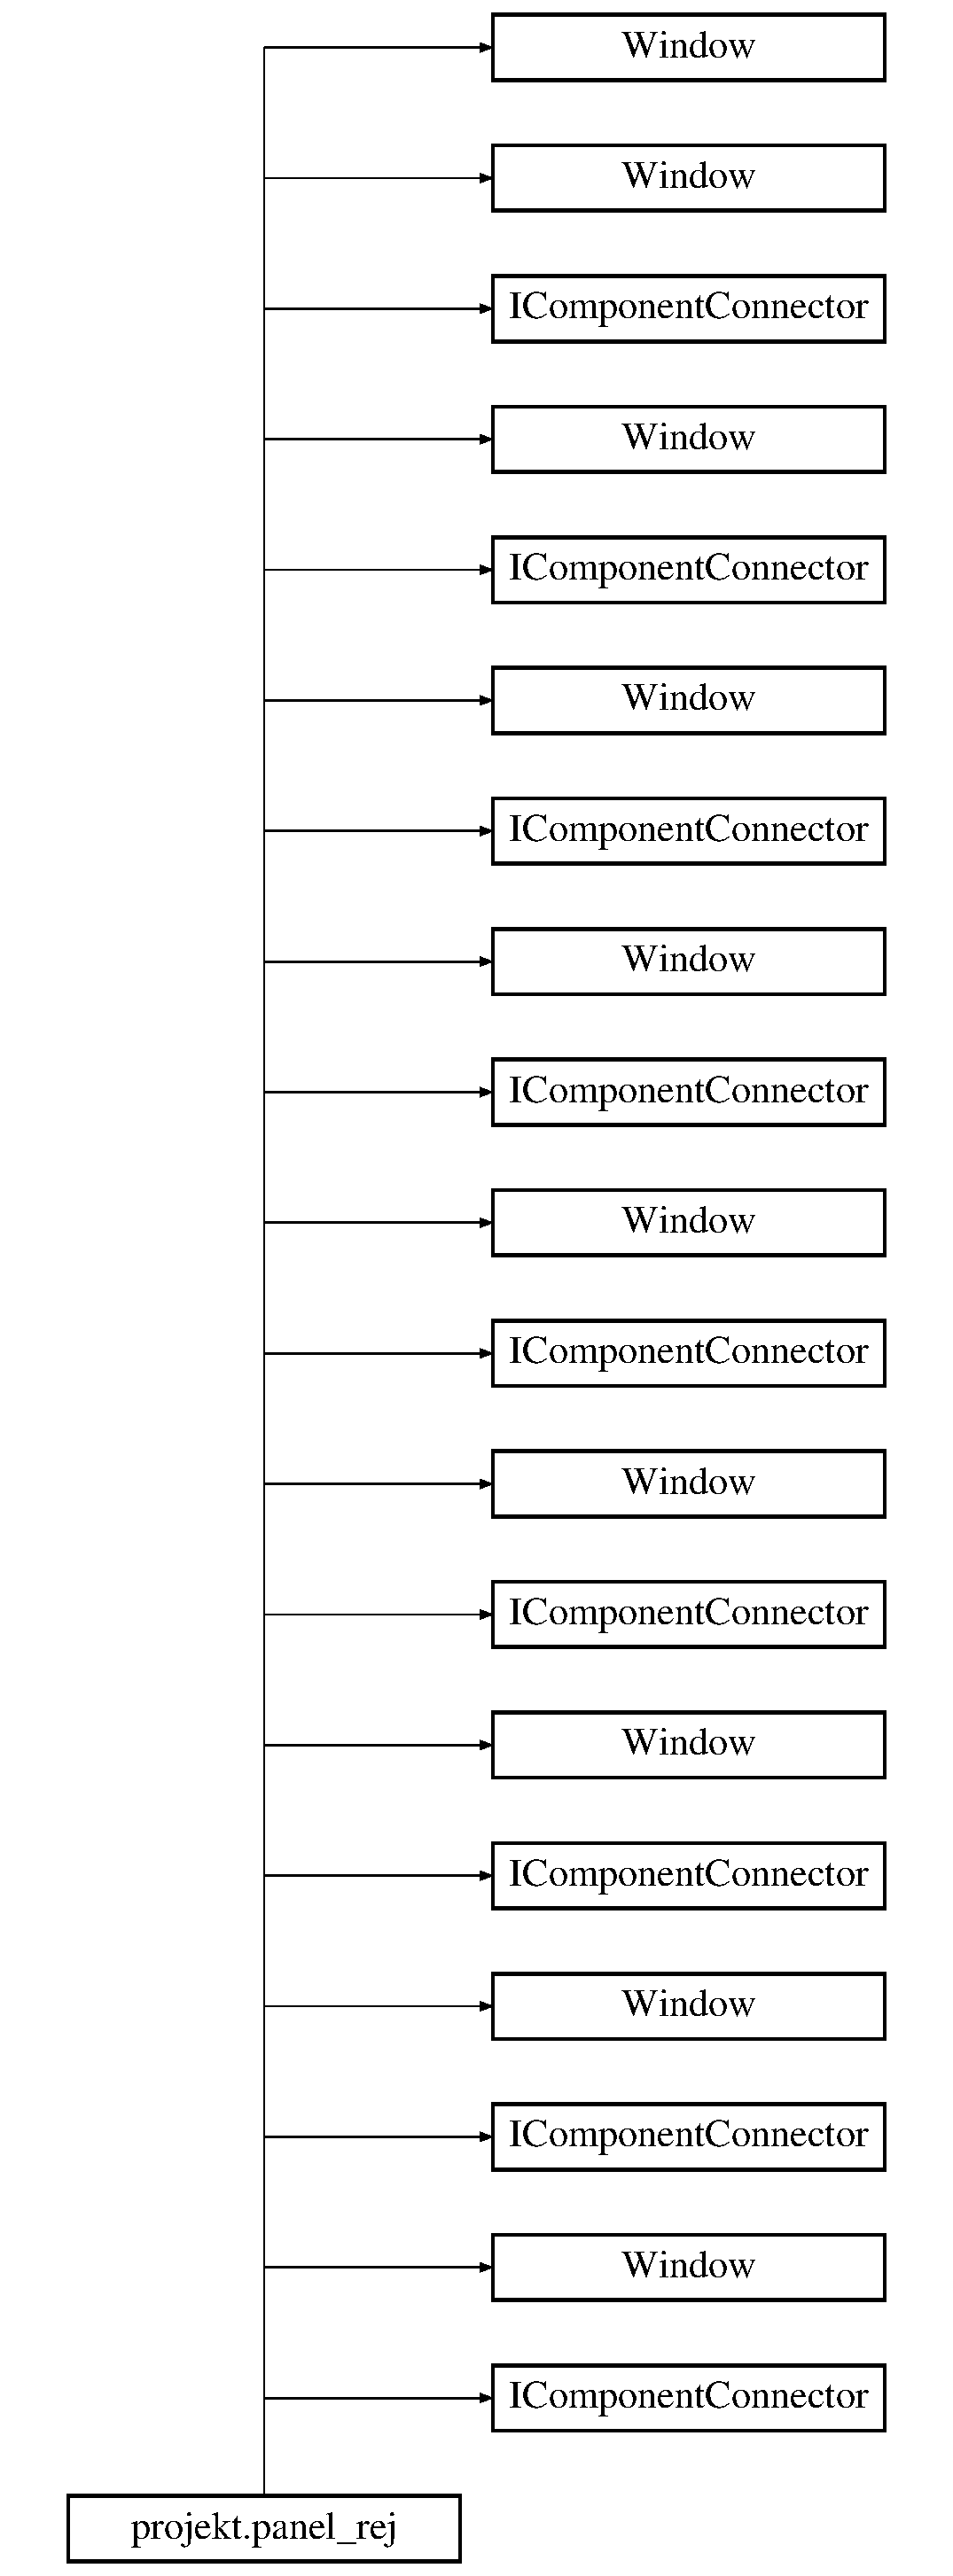
\includegraphics[height=12.000000cm]{classprojekt_1_1panel__rej}
\end{center}
\end{figure}
\subsection*{Public Member Functions}
\begin{DoxyCompactItemize}
\item 
void \mbox{\hyperlink{classprojekt_1_1panel__rej_a603f590d84827e1d551b3f781d6c1f28}{Initialize\+Component}} ()
\begin{DoxyCompactList}\small\item\em Initialize\+Component \end{DoxyCompactList}\item 
void \mbox{\hyperlink{classprojekt_1_1panel__rej_a603f590d84827e1d551b3f781d6c1f28}{Initialize\+Component}} ()
\begin{DoxyCompactList}\small\item\em Initialize\+Component \end{DoxyCompactList}\item 
void \mbox{\hyperlink{classprojekt_1_1panel__rej_a603f590d84827e1d551b3f781d6c1f28}{Initialize\+Component}} ()
\begin{DoxyCompactList}\small\item\em Initialize\+Component \end{DoxyCompactList}\item 
void \mbox{\hyperlink{classprojekt_1_1panel__rej_a603f590d84827e1d551b3f781d6c1f28}{Initialize\+Component}} ()
\begin{DoxyCompactList}\small\item\em Initialize\+Component \end{DoxyCompactList}\item 
void \mbox{\hyperlink{classprojekt_1_1panel__rej_a603f590d84827e1d551b3f781d6c1f28}{Initialize\+Component}} ()
\begin{DoxyCompactList}\small\item\em Initialize\+Component \end{DoxyCompactList}\item 
void \mbox{\hyperlink{classprojekt_1_1panel__rej_a603f590d84827e1d551b3f781d6c1f28}{Initialize\+Component}} ()
\begin{DoxyCompactList}\small\item\em Initialize\+Component \end{DoxyCompactList}\item 
void \mbox{\hyperlink{classprojekt_1_1panel__rej_a603f590d84827e1d551b3f781d6c1f28}{Initialize\+Component}} ()
\begin{DoxyCompactList}\small\item\em Initialize\+Component \end{DoxyCompactList}\item 
void \mbox{\hyperlink{classprojekt_1_1panel__rej_a603f590d84827e1d551b3f781d6c1f28}{Initialize\+Component}} ()
\begin{DoxyCompactList}\small\item\em Initialize\+Component \end{DoxyCompactList}\item 
void \mbox{\hyperlink{classprojekt_1_1panel__rej_a603f590d84827e1d551b3f781d6c1f28}{Initialize\+Component}} ()
\begin{DoxyCompactList}\small\item\em Initialize\+Component \end{DoxyCompactList}\item 
\mbox{\hyperlink{classprojekt_1_1panel__rej_ac8e3a97468a6c4fe9f49b37721a7e265}{panel\+\_\+rej}} ()
\begin{DoxyCompactList}\small\item\em metoda, gdzie jest połączenie z bazą danych przy pomocy ścieżki do pliku wykorzysując klasę System.\+String \end{DoxyCompactList}\item 
void \mbox{\hyperlink{classprojekt_1_1panel__rej_aea82627753b6eee1ed0fef05c784fadc}{b\+\_\+zarejestruj\+\_\+\+Click}} (object sender, Routed\+Event\+Args e)
\begin{DoxyCompactList}\small\item\em funkcja b\+\_\+zarejestruj\+\_\+\+Click -\/ po użyciu przycisku dane po spełnieniu warunku zapisywane są do tabeli użytkownicy w bazie danych (służy do tego odwołanie sql w kodzie) \end{DoxyCompactList}\end{DoxyCompactItemize}


\subsection{Detailed Description}
\mbox{\hyperlink{classprojekt_1_1panel__rej}{panel\+\_\+rej}} 

panel rejestracyjny 

\subsection{Constructor \& Destructor Documentation}
\mbox{\Hypertarget{classprojekt_1_1panel__rej_ac8e3a97468a6c4fe9f49b37721a7e265}\label{classprojekt_1_1panel__rej_ac8e3a97468a6c4fe9f49b37721a7e265}} 
\index{projekt\+::panel\+\_\+rej@{projekt\+::panel\+\_\+rej}!panel\+\_\+rej@{panel\+\_\+rej}}
\index{panel\+\_\+rej@{panel\+\_\+rej}!projekt\+::panel\+\_\+rej@{projekt\+::panel\+\_\+rej}}
\subsubsection{\texorpdfstring{panel\+\_\+rej()}{panel\_rej()}}
{\footnotesize\ttfamily projekt.\+panel\+\_\+rej.\+panel\+\_\+rej (\begin{DoxyParamCaption}{ }\end{DoxyParamCaption})\hspace{0.3cm}{\ttfamily [inline]}}



metoda, gdzie jest połączenie z bazą danych przy pomocy ścieżki do pliku wykorzysując klasę System.\+String 



\subsection{Member Function Documentation}
\mbox{\Hypertarget{classprojekt_1_1panel__rej_aea82627753b6eee1ed0fef05c784fadc}\label{classprojekt_1_1panel__rej_aea82627753b6eee1ed0fef05c784fadc}} 
\index{projekt\+::panel\+\_\+rej@{projekt\+::panel\+\_\+rej}!b\+\_\+zarejestruj\+\_\+\+Click@{b\+\_\+zarejestruj\+\_\+\+Click}}
\index{b\+\_\+zarejestruj\+\_\+\+Click@{b\+\_\+zarejestruj\+\_\+\+Click}!projekt\+::panel\+\_\+rej@{projekt\+::panel\+\_\+rej}}
\subsubsection{\texorpdfstring{b\+\_\+zarejestruj\+\_\+\+Click()}{b\_zarejestruj\_Click()}}
{\footnotesize\ttfamily void projekt.\+panel\+\_\+rej.\+b\+\_\+zarejestruj\+\_\+\+Click (\begin{DoxyParamCaption}\item[{object}]{sender,  }\item[{Routed\+Event\+Args}]{e }\end{DoxyParamCaption})\hspace{0.3cm}{\ttfamily [inline]}}



funkcja b\+\_\+zarejestruj\+\_\+\+Click -\/ po użyciu przycisku dane po spełnieniu warunku zapisywane są do tabeli użytkownicy w bazie danych (służy do tego odwołanie sql w kodzie) 

tworzę zmienną int count równą 0(będzie to odzwierciedleniem loginów i haseł w bazie, dzięki temu weryfikuje po kolei loginy i hasła wpisane do bazy)

przy pomocy pętli while poruszam się rosnąco po rekordach naszej bazy

count++;

instrukcja if(jesli loginów i haseł jest mniej niż 1 zapisuje konto)

command.\+Command\+Text = \char`\"{}insert into Uzytkownicy(\+Login, Haslo) values(\textquotesingle{}\char`\"{}+txt\+\_\+login.Text + \char`\"{}\textquotesingle{},\textquotesingle{}\char`\"{} + txt\+\_\+password.\+Password +\char`\"{}\textquotesingle{},)\char`\"{}; // odwołanie do bazy danych aby po spełnieniu warunku if nasze dane zostają zapisane w tabeli w odpowiednich kolumnach

rozpisanie kolumn

zwraca informację o wykonanym zadaniu do bazy danych(czyli zapisuje login i hasło do bazy)

connection.\+Close zamyka połączenie z bazą danych po spełnieniu warunku

jeśli przy logowaniu wartość takiego samego loginu i hasła jest taka sama, zwraca komunikat o istniejącym loginie lub haśle

baza danych dysponuje już takimi danymi ~\newline
~\newline
~\newline
 jeśli przy logowaniu wartość takiego samego loginu i hasła jest taka sama, zwraca komunikat o istniejącym loginie lub haśle

baza danych dysponuje już takimi danymi ~\newline
 else czyli pozostałe przypadki, jeśli użytkownik wpisze niepoprawne wartości do textboxa loginu lub hasła wyrzuci komunikat o niepoprawnych danych \mbox{\Hypertarget{classprojekt_1_1panel__rej_a603f590d84827e1d551b3f781d6c1f28}\label{classprojekt_1_1panel__rej_a603f590d84827e1d551b3f781d6c1f28}} 
\index{projekt\+::panel\+\_\+rej@{projekt\+::panel\+\_\+rej}!Initialize\+Component@{Initialize\+Component}}
\index{Initialize\+Component@{Initialize\+Component}!projekt\+::panel\+\_\+rej@{projekt\+::panel\+\_\+rej}}
\subsubsection{\texorpdfstring{Initialize\+Component()}{InitializeComponent()}\hspace{0.1cm}{\footnotesize\ttfamily [1/9]}}
{\footnotesize\ttfamily void projekt.\+panel\+\_\+rej.\+Initialize\+Component (\begin{DoxyParamCaption}{ }\end{DoxyParamCaption})\hspace{0.3cm}{\ttfamily [inline]}}



Initialize\+Component 

\mbox{\Hypertarget{classprojekt_1_1panel__rej_a603f590d84827e1d551b3f781d6c1f28}\label{classprojekt_1_1panel__rej_a603f590d84827e1d551b3f781d6c1f28}} 
\index{projekt\+::panel\+\_\+rej@{projekt\+::panel\+\_\+rej}!Initialize\+Component@{Initialize\+Component}}
\index{Initialize\+Component@{Initialize\+Component}!projekt\+::panel\+\_\+rej@{projekt\+::panel\+\_\+rej}}
\subsubsection{\texorpdfstring{Initialize\+Component()}{InitializeComponent()}\hspace{0.1cm}{\footnotesize\ttfamily [2/9]}}
{\footnotesize\ttfamily void projekt.\+panel\+\_\+rej.\+Initialize\+Component (\begin{DoxyParamCaption}{ }\end{DoxyParamCaption})\hspace{0.3cm}{\ttfamily [inline]}}



Initialize\+Component 

\mbox{\Hypertarget{classprojekt_1_1panel__rej_a603f590d84827e1d551b3f781d6c1f28}\label{classprojekt_1_1panel__rej_a603f590d84827e1d551b3f781d6c1f28}} 
\index{projekt\+::panel\+\_\+rej@{projekt\+::panel\+\_\+rej}!Initialize\+Component@{Initialize\+Component}}
\index{Initialize\+Component@{Initialize\+Component}!projekt\+::panel\+\_\+rej@{projekt\+::panel\+\_\+rej}}
\subsubsection{\texorpdfstring{Initialize\+Component()}{InitializeComponent()}\hspace{0.1cm}{\footnotesize\ttfamily [3/9]}}
{\footnotesize\ttfamily void projekt.\+panel\+\_\+rej.\+Initialize\+Component (\begin{DoxyParamCaption}{ }\end{DoxyParamCaption})\hspace{0.3cm}{\ttfamily [inline]}}



Initialize\+Component 

\mbox{\Hypertarget{classprojekt_1_1panel__rej_a603f590d84827e1d551b3f781d6c1f28}\label{classprojekt_1_1panel__rej_a603f590d84827e1d551b3f781d6c1f28}} 
\index{projekt\+::panel\+\_\+rej@{projekt\+::panel\+\_\+rej}!Initialize\+Component@{Initialize\+Component}}
\index{Initialize\+Component@{Initialize\+Component}!projekt\+::panel\+\_\+rej@{projekt\+::panel\+\_\+rej}}
\subsubsection{\texorpdfstring{Initialize\+Component()}{InitializeComponent()}\hspace{0.1cm}{\footnotesize\ttfamily [4/9]}}
{\footnotesize\ttfamily void projekt.\+panel\+\_\+rej.\+Initialize\+Component (\begin{DoxyParamCaption}{ }\end{DoxyParamCaption})\hspace{0.3cm}{\ttfamily [inline]}}



Initialize\+Component 

\mbox{\Hypertarget{classprojekt_1_1panel__rej_a603f590d84827e1d551b3f781d6c1f28}\label{classprojekt_1_1panel__rej_a603f590d84827e1d551b3f781d6c1f28}} 
\index{projekt\+::panel\+\_\+rej@{projekt\+::panel\+\_\+rej}!Initialize\+Component@{Initialize\+Component}}
\index{Initialize\+Component@{Initialize\+Component}!projekt\+::panel\+\_\+rej@{projekt\+::panel\+\_\+rej}}
\subsubsection{\texorpdfstring{Initialize\+Component()}{InitializeComponent()}\hspace{0.1cm}{\footnotesize\ttfamily [5/9]}}
{\footnotesize\ttfamily void projekt.\+panel\+\_\+rej.\+Initialize\+Component (\begin{DoxyParamCaption}{ }\end{DoxyParamCaption})\hspace{0.3cm}{\ttfamily [inline]}}



Initialize\+Component 

\mbox{\Hypertarget{classprojekt_1_1panel__rej_a603f590d84827e1d551b3f781d6c1f28}\label{classprojekt_1_1panel__rej_a603f590d84827e1d551b3f781d6c1f28}} 
\index{projekt\+::panel\+\_\+rej@{projekt\+::panel\+\_\+rej}!Initialize\+Component@{Initialize\+Component}}
\index{Initialize\+Component@{Initialize\+Component}!projekt\+::panel\+\_\+rej@{projekt\+::panel\+\_\+rej}}
\subsubsection{\texorpdfstring{Initialize\+Component()}{InitializeComponent()}\hspace{0.1cm}{\footnotesize\ttfamily [6/9]}}
{\footnotesize\ttfamily void projekt.\+panel\+\_\+rej.\+Initialize\+Component (\begin{DoxyParamCaption}{ }\end{DoxyParamCaption})\hspace{0.3cm}{\ttfamily [inline]}}



Initialize\+Component 

\mbox{\Hypertarget{classprojekt_1_1panel__rej_a603f590d84827e1d551b3f781d6c1f28}\label{classprojekt_1_1panel__rej_a603f590d84827e1d551b3f781d6c1f28}} 
\index{projekt\+::panel\+\_\+rej@{projekt\+::panel\+\_\+rej}!Initialize\+Component@{Initialize\+Component}}
\index{Initialize\+Component@{Initialize\+Component}!projekt\+::panel\+\_\+rej@{projekt\+::panel\+\_\+rej}}
\subsubsection{\texorpdfstring{Initialize\+Component()}{InitializeComponent()}\hspace{0.1cm}{\footnotesize\ttfamily [7/9]}}
{\footnotesize\ttfamily void projekt.\+panel\+\_\+rej.\+Initialize\+Component (\begin{DoxyParamCaption}{ }\end{DoxyParamCaption})\hspace{0.3cm}{\ttfamily [inline]}}



Initialize\+Component 

\mbox{\Hypertarget{classprojekt_1_1panel__rej_a603f590d84827e1d551b3f781d6c1f28}\label{classprojekt_1_1panel__rej_a603f590d84827e1d551b3f781d6c1f28}} 
\index{projekt\+::panel\+\_\+rej@{projekt\+::panel\+\_\+rej}!Initialize\+Component@{Initialize\+Component}}
\index{Initialize\+Component@{Initialize\+Component}!projekt\+::panel\+\_\+rej@{projekt\+::panel\+\_\+rej}}
\subsubsection{\texorpdfstring{Initialize\+Component()}{InitializeComponent()}\hspace{0.1cm}{\footnotesize\ttfamily [8/9]}}
{\footnotesize\ttfamily void projekt.\+panel\+\_\+rej.\+Initialize\+Component (\begin{DoxyParamCaption}{ }\end{DoxyParamCaption})\hspace{0.3cm}{\ttfamily [inline]}}



Initialize\+Component 

\mbox{\Hypertarget{classprojekt_1_1panel__rej_a603f590d84827e1d551b3f781d6c1f28}\label{classprojekt_1_1panel__rej_a603f590d84827e1d551b3f781d6c1f28}} 
\index{projekt\+::panel\+\_\+rej@{projekt\+::panel\+\_\+rej}!Initialize\+Component@{Initialize\+Component}}
\index{Initialize\+Component@{Initialize\+Component}!projekt\+::panel\+\_\+rej@{projekt\+::panel\+\_\+rej}}
\subsubsection{\texorpdfstring{Initialize\+Component()}{InitializeComponent()}\hspace{0.1cm}{\footnotesize\ttfamily [9/9]}}
{\footnotesize\ttfamily void projekt.\+panel\+\_\+rej.\+Initialize\+Component (\begin{DoxyParamCaption}{ }\end{DoxyParamCaption})\hspace{0.3cm}{\ttfamily [inline]}}



Initialize\+Component 



The documentation for this class was generated from the following files\+:\begin{DoxyCompactItemize}
\item 
projekt/obj/\+Debug/\mbox{\hyperlink{_debug_2panel__rej_8g_8cs}{panel\+\_\+rej.\+g.\+cs}}\item 
projekt/obj/\+Debug/\mbox{\hyperlink{_debug_2panel__rej_8g_8i_8cs}{panel\+\_\+rej.\+g.\+i.\+cs}}\item 
projekt/\mbox{\hyperlink{panel__rej_8xaml_8cs}{panel\+\_\+rej.\+xaml.\+cs}}\end{DoxyCompactItemize}

\hypertarget{classprojekt_1_1_tests_1_1panel__rej_tests}{}\section{projekt.\+Tests.\+panel\+\_\+rej\+Tests Class Reference}
\label{classprojekt_1_1_tests_1_1panel__rej_tests}\index{projekt.\+Tests.\+panel\+\_\+rej\+Tests@{projekt.\+Tests.\+panel\+\_\+rej\+Tests}}
\subsection*{Public Member Functions}
\begin{DoxyCompactItemize}
\item 
void \mbox{\hyperlink{classprojekt_1_1_tests_1_1panel__rej_tests_acd26dd99e18d73015373885a53e41055}{Test\+Rejestracjidobazy}} ()
\end{DoxyCompactItemize}


\subsection{Member Function Documentation}
\mbox{\Hypertarget{classprojekt_1_1_tests_1_1panel__rej_tests_acd26dd99e18d73015373885a53e41055}\label{classprojekt_1_1_tests_1_1panel__rej_tests_acd26dd99e18d73015373885a53e41055}} 
\index{projekt\+::\+Tests\+::panel\+\_\+rej\+Tests@{projekt\+::\+Tests\+::panel\+\_\+rej\+Tests}!Test\+Rejestracjidobazy@{Test\+Rejestracjidobazy}}
\index{Test\+Rejestracjidobazy@{Test\+Rejestracjidobazy}!projekt\+::\+Tests\+::panel\+\_\+rej\+Tests@{projekt\+::\+Tests\+::panel\+\_\+rej\+Tests}}
\subsubsection{\texorpdfstring{Test\+Rejestracjidobazy()}{TestRejestracjidobazy()}}
{\footnotesize\ttfamily void projekt.\+Tests.\+panel\+\_\+rej\+Tests.\+Test\+Rejestracjidobazy (\begin{DoxyParamCaption}{ }\end{DoxyParamCaption})\hspace{0.3cm}{\ttfamily [inline]}}

rozpisanie kolumn

zwraca informację o wykonanym zadaniu do bazy danych(czyli zapisuje login i hasło do bazy) 

The documentation for this class was generated from the following file\+:\begin{DoxyCompactItemize}
\item 
projekt\+Tests2/\mbox{\hyperlink{panel__rej_tests_8cs}{panel\+\_\+rej\+Tests.\+cs}}\end{DoxyCompactItemize}

\section{projekt.\+pole\+\_\+gry Class Reference}
\label{classprojekt_1_1pole__gry}\index{projekt.\+pole\+\_\+gry@{projekt.\+pole\+\_\+gry}}


\doxyref{pole\+\_\+gry}{p.}{classprojekt_1_1pole__gry}  


Inheritance diagram for projekt.\+pole\+\_\+gry\+:\begin{figure}[H]
\begin{center}
\leavevmode
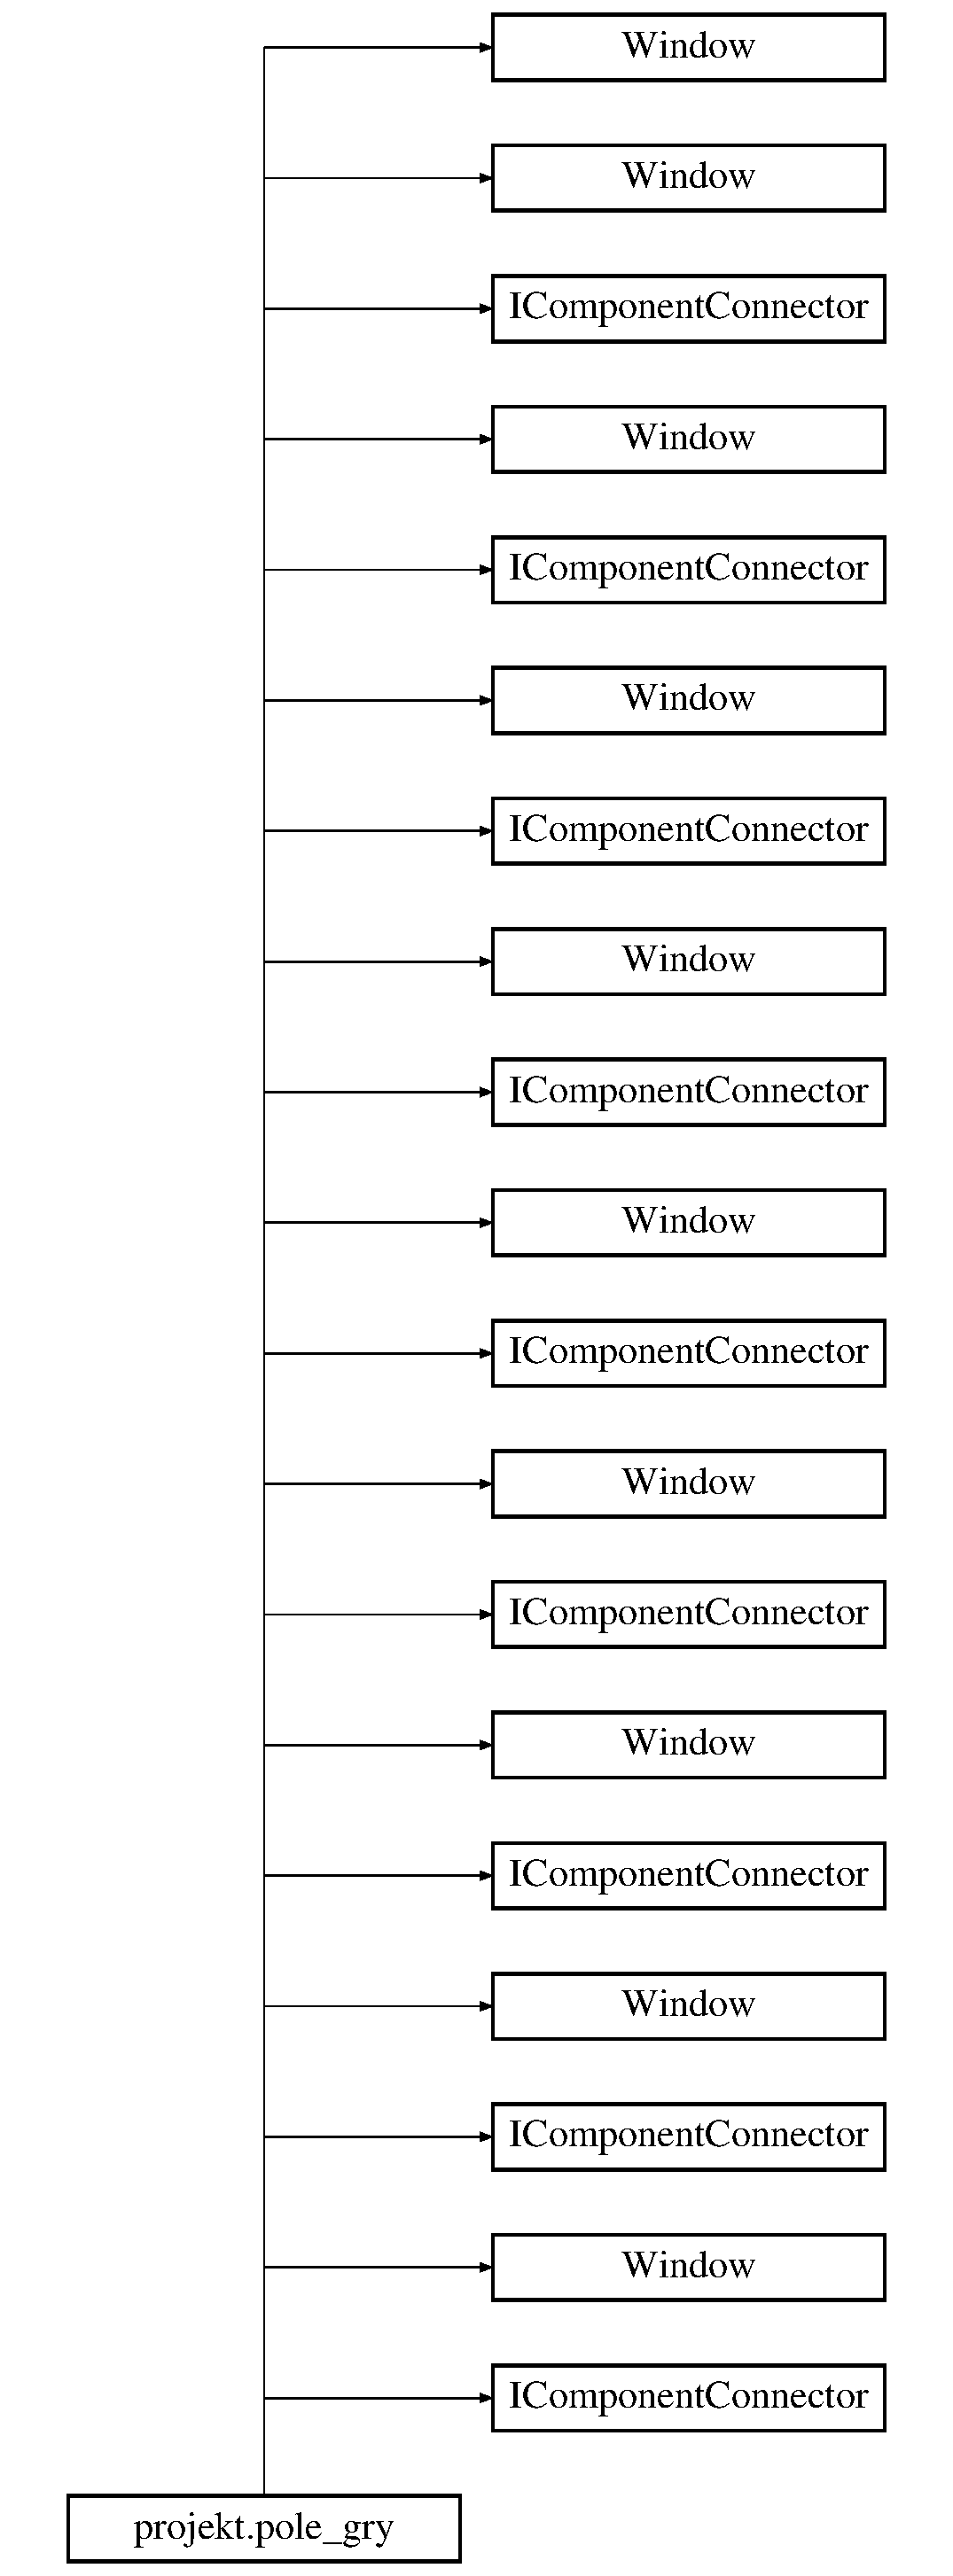
\includegraphics[height=12.000000cm]{classprojekt_1_1pole__gry}
\end{center}
\end{figure}
\subsection*{Public Member Functions}
\begin{DoxyCompactItemize}
\item 
void \textbf{ Initialize\+Component} ()
\begin{DoxyCompactList}\small\item\em Initialize\+Component \end{DoxyCompactList}\item 
void \textbf{ Initialize\+Component} ()
\begin{DoxyCompactList}\small\item\em Initialize\+Component \end{DoxyCompactList}\item 
void \textbf{ Initialize\+Component} ()
\begin{DoxyCompactList}\small\item\em Initialize\+Component \end{DoxyCompactList}\item 
void \textbf{ Initialize\+Component} ()
\begin{DoxyCompactList}\small\item\em Initialize\+Component \end{DoxyCompactList}\item 
void \textbf{ Initialize\+Component} ()
\begin{DoxyCompactList}\small\item\em Initialize\+Component \end{DoxyCompactList}\item 
void \textbf{ Initialize\+Component} ()
\begin{DoxyCompactList}\small\item\em Initialize\+Component \end{DoxyCompactList}\item 
void \textbf{ Initialize\+Component} ()
\begin{DoxyCompactList}\small\item\em Initialize\+Component \end{DoxyCompactList}\item 
void \textbf{ Initialize\+Component} ()
\begin{DoxyCompactList}\small\item\em Initialize\+Component \end{DoxyCompactList}\item 
void \textbf{ Initialize\+Component} ()
\begin{DoxyCompactList}\small\item\em Initialize\+Component \end{DoxyCompactList}\item 
\textbf{ pole\+\_\+gry} ()
\begin{DoxyCompactList}\small\item\em private Ole\+Db\+Connection connection = new Ole\+Db\+Connection(); połączenie prywatne do bazy danych z klasy \doxyref{pole\+\_\+gry}{p.}{classprojekt_1_1pole__gry} \end{DoxyCompactList}\end{DoxyCompactItemize}


\subsection{Detailed Description}
\doxyref{pole\+\_\+gry}{p.}{classprojekt_1_1pole__gry} 

Logika interakcji dla klasy pole gry 

clasa \doxyref{pole\+\_\+gry}{p.}{classprojekt_1_1pole__gry} 

Definition at line 41 of file pole\+\_\+gry.\+g.\+cs.



\subsection{Constructor \& Destructor Documentation}
\mbox{\label{classprojekt_1_1pole__gry_a5a66280013aef4e5a38ae1d0928d978a}} 
\index{projekt\+::pole\+\_\+gry@{projekt\+::pole\+\_\+gry}!pole\+\_\+gry@{pole\+\_\+gry}}
\index{pole\+\_\+gry@{pole\+\_\+gry}!projekt\+::pole\+\_\+gry@{projekt\+::pole\+\_\+gry}}
\subsubsection{pole\+\_\+gry()}
{\footnotesize\ttfamily projekt.\+pole\+\_\+gry.\+pole\+\_\+gry (\begin{DoxyParamCaption}{ }\end{DoxyParamCaption})\hspace{0.3cm}{\ttfamily [inline]}}



private Ole\+Db\+Connection connection = new Ole\+Db\+Connection(); połączenie prywatne do bazy danych z klasy \doxyref{pole\+\_\+gry}{p.}{classprojekt_1_1pole__gry} 

odwółanine do klasy odwolanie do lokalnej bazy danych\+\_\+z adresem

odwolanie do metody

odwolanie do metody 

Definition at line 27 of file pole\+\_\+gry.\+xaml.\+cs.



\subsection{Member Function Documentation}
\mbox{\label{classprojekt_1_1pole__gry_acb91309f48624fdcd50a6f023a810f02}} 
\index{projekt\+::pole\+\_\+gry@{projekt\+::pole\+\_\+gry}!Initialize\+Component@{Initialize\+Component}}
\index{Initialize\+Component@{Initialize\+Component}!projekt\+::pole\+\_\+gry@{projekt\+::pole\+\_\+gry}}
\subsubsection{Initialize\+Component()\hspace{0.1cm}{\footnotesize\ttfamily [1/9]}}
{\footnotesize\ttfamily void projekt.\+pole\+\_\+gry.\+Initialize\+Component (\begin{DoxyParamCaption}{ }\end{DoxyParamCaption})\hspace{0.3cm}{\ttfamily [inline]}}



Initialize\+Component 



Definition at line 202 of file pole\+\_\+gry.\+g.\+cs.

\mbox{\label{classprojekt_1_1pole__gry_acb91309f48624fdcd50a6f023a810f02}} 
\index{projekt\+::pole\+\_\+gry@{projekt\+::pole\+\_\+gry}!Initialize\+Component@{Initialize\+Component}}
\index{Initialize\+Component@{Initialize\+Component}!projekt\+::pole\+\_\+gry@{projekt\+::pole\+\_\+gry}}
\subsubsection{Initialize\+Component()\hspace{0.1cm}{\footnotesize\ttfamily [2/9]}}
{\footnotesize\ttfamily void projekt.\+pole\+\_\+gry.\+Initialize\+Component (\begin{DoxyParamCaption}{ }\end{DoxyParamCaption})\hspace{0.3cm}{\ttfamily [inline]}}



Initialize\+Component 



Definition at line 202 of file pole\+\_\+gry.\+g.\+i.\+cs.

\mbox{\label{classprojekt_1_1pole__gry_acb91309f48624fdcd50a6f023a810f02}} 
\index{projekt\+::pole\+\_\+gry@{projekt\+::pole\+\_\+gry}!Initialize\+Component@{Initialize\+Component}}
\index{Initialize\+Component@{Initialize\+Component}!projekt\+::pole\+\_\+gry@{projekt\+::pole\+\_\+gry}}
\subsubsection{Initialize\+Component()\hspace{0.1cm}{\footnotesize\ttfamily [3/9]}}
{\footnotesize\ttfamily void projekt.\+pole\+\_\+gry.\+Initialize\+Component (\begin{DoxyParamCaption}{ }\end{DoxyParamCaption})\hspace{0.3cm}{\ttfamily [inline]}}



Initialize\+Component 



Definition at line 210 of file pole\+\_\+gry.\+g.\+cs.

\mbox{\label{classprojekt_1_1pole__gry_acb91309f48624fdcd50a6f023a810f02}} 
\index{projekt\+::pole\+\_\+gry@{projekt\+::pole\+\_\+gry}!Initialize\+Component@{Initialize\+Component}}
\index{Initialize\+Component@{Initialize\+Component}!projekt\+::pole\+\_\+gry@{projekt\+::pole\+\_\+gry}}
\subsubsection{Initialize\+Component()\hspace{0.1cm}{\footnotesize\ttfamily [4/9]}}
{\footnotesize\ttfamily void projekt.\+pole\+\_\+gry.\+Initialize\+Component (\begin{DoxyParamCaption}{ }\end{DoxyParamCaption})\hspace{0.3cm}{\ttfamily [inline]}}



Initialize\+Component 



Definition at line 210 of file pole\+\_\+gry.\+g.\+i.\+cs.

\mbox{\label{classprojekt_1_1pole__gry_acb91309f48624fdcd50a6f023a810f02}} 
\index{projekt\+::pole\+\_\+gry@{projekt\+::pole\+\_\+gry}!Initialize\+Component@{Initialize\+Component}}
\index{Initialize\+Component@{Initialize\+Component}!projekt\+::pole\+\_\+gry@{projekt\+::pole\+\_\+gry}}
\subsubsection{Initialize\+Component()\hspace{0.1cm}{\footnotesize\ttfamily [5/9]}}
{\footnotesize\ttfamily void projekt.\+pole\+\_\+gry.\+Initialize\+Component (\begin{DoxyParamCaption}{ }\end{DoxyParamCaption})\hspace{0.3cm}{\ttfamily [inline]}}



Initialize\+Component 



Definition at line 210 of file pole\+\_\+gry.\+g.\+cs.

\mbox{\label{classprojekt_1_1pole__gry_acb91309f48624fdcd50a6f023a810f02}} 
\index{projekt\+::pole\+\_\+gry@{projekt\+::pole\+\_\+gry}!Initialize\+Component@{Initialize\+Component}}
\index{Initialize\+Component@{Initialize\+Component}!projekt\+::pole\+\_\+gry@{projekt\+::pole\+\_\+gry}}
\subsubsection{Initialize\+Component()\hspace{0.1cm}{\footnotesize\ttfamily [6/9]}}
{\footnotesize\ttfamily void projekt.\+pole\+\_\+gry.\+Initialize\+Component (\begin{DoxyParamCaption}{ }\end{DoxyParamCaption})\hspace{0.3cm}{\ttfamily [inline]}}



Initialize\+Component 



Definition at line 210 of file pole\+\_\+gry.\+g.\+i.\+cs.

\mbox{\label{classprojekt_1_1pole__gry_acb91309f48624fdcd50a6f023a810f02}} 
\index{projekt\+::pole\+\_\+gry@{projekt\+::pole\+\_\+gry}!Initialize\+Component@{Initialize\+Component}}
\index{Initialize\+Component@{Initialize\+Component}!projekt\+::pole\+\_\+gry@{projekt\+::pole\+\_\+gry}}
\subsubsection{Initialize\+Component()\hspace{0.1cm}{\footnotesize\ttfamily [7/9]}}
{\footnotesize\ttfamily void projekt.\+pole\+\_\+gry.\+Initialize\+Component (\begin{DoxyParamCaption}{ }\end{DoxyParamCaption})\hspace{0.3cm}{\ttfamily [inline]}}



Initialize\+Component 



Definition at line 210 of file pole\+\_\+gry.\+g.\+i.\+cs.

\mbox{\label{classprojekt_1_1pole__gry_acb91309f48624fdcd50a6f023a810f02}} 
\index{projekt\+::pole\+\_\+gry@{projekt\+::pole\+\_\+gry}!Initialize\+Component@{Initialize\+Component}}
\index{Initialize\+Component@{Initialize\+Component}!projekt\+::pole\+\_\+gry@{projekt\+::pole\+\_\+gry}}
\subsubsection{Initialize\+Component()\hspace{0.1cm}{\footnotesize\ttfamily [8/9]}}
{\footnotesize\ttfamily void projekt.\+pole\+\_\+gry.\+Initialize\+Component (\begin{DoxyParamCaption}{ }\end{DoxyParamCaption})\hspace{0.3cm}{\ttfamily [inline]}}



Initialize\+Component 



Definition at line 210 of file pole\+\_\+gry.\+g.\+cs.

\mbox{\label{classprojekt_1_1pole__gry_acb91309f48624fdcd50a6f023a810f02}} 
\index{projekt\+::pole\+\_\+gry@{projekt\+::pole\+\_\+gry}!Initialize\+Component@{Initialize\+Component}}
\index{Initialize\+Component@{Initialize\+Component}!projekt\+::pole\+\_\+gry@{projekt\+::pole\+\_\+gry}}
\subsubsection{Initialize\+Component()\hspace{0.1cm}{\footnotesize\ttfamily [9/9]}}
{\footnotesize\ttfamily void projekt.\+pole\+\_\+gry.\+Initialize\+Component (\begin{DoxyParamCaption}{ }\end{DoxyParamCaption})\hspace{0.3cm}{\ttfamily [inline]}}



Initialize\+Component 



Definition at line 210 of file pole\+\_\+gry.\+g.\+i.\+cs.



The documentation for this class was generated from the following files\+:\begin{DoxyCompactItemize}
\item 
projekt/obj/\+Debug/\textbf{ pole\+\_\+gry.\+g.\+cs}\item 
projekt/obj/\+Debug/\textbf{ pole\+\_\+gry.\+g.\+i.\+cs}\item 
projekt/\textbf{ pole\+\_\+gry.\+xaml.\+cs}\end{DoxyCompactItemize}

\hypertarget{classprojekt_1_1_tests_1_1pole__gry_tests}{}\section{projekt.\+Tests.\+pole\+\_\+gry\+Tests Class Reference}
\label{classprojekt_1_1_tests_1_1pole__gry_tests}\index{projekt.\+Tests.\+pole\+\_\+gry\+Tests@{projekt.\+Tests.\+pole\+\_\+gry\+Tests}}


 


\subsection*{Public Member Functions}
\begin{DoxyCompactItemize}
\item 
void \mbox{\hyperlink{classprojekt_1_1_tests_1_1pole__gry_tests_a452be98c348cb92cdfb70eadeb3df1d0}{losuj\+Test}} ()
\begin{DoxyCompactList}\small\item\em metoda sprawdzająca losowość oraz czy poprawnie działa wybór gracza, który rozpoczyna rozgrywkę \end{DoxyCompactList}\item 
void \mbox{\hyperlink{classprojekt_1_1_tests_1_1pole__gry_tests_ad19d9a740af149c53c775875154982db}{Spr\+\_\+zapis\+\_\+do\+\_\+bazy\+\_\+\+Wynik}} ()
\begin{DoxyCompactList}\small\item\em metoda testująca zapis punktów do bazy danych przypisanych odpowiedniemu użytkownikowi \end{DoxyCompactList}\end{DoxyCompactItemize}


\subsection{Detailed Description}


klasa testująca \mbox{\hyperlink{classprojekt_1_1_tests_1_1pole__gry_tests}{pole\+\_\+gry\+Tests}} 

\subsection{Member Function Documentation}
\mbox{\Hypertarget{classprojekt_1_1_tests_1_1pole__gry_tests_a452be98c348cb92cdfb70eadeb3df1d0}\label{classprojekt_1_1_tests_1_1pole__gry_tests_a452be98c348cb92cdfb70eadeb3df1d0}} 
\index{projekt\+::\+Tests\+::pole\+\_\+gry\+Tests@{projekt\+::\+Tests\+::pole\+\_\+gry\+Tests}!losuj\+Test@{losuj\+Test}}
\index{losuj\+Test@{losuj\+Test}!projekt\+::\+Tests\+::pole\+\_\+gry\+Tests@{projekt\+::\+Tests\+::pole\+\_\+gry\+Tests}}
\subsubsection{\texorpdfstring{losuj\+Test()}{losujTest()}}
{\footnotesize\ttfamily void projekt.\+Tests.\+pole\+\_\+gry\+Tests.\+losuj\+Test (\begin{DoxyParamCaption}{ }\end{DoxyParamCaption})\hspace{0.3cm}{\ttfamily [inline]}}



metoda sprawdzająca losowość oraz czy poprawnie działa wybór gracza, który rozpoczyna rozgrywkę 

\mbox{\Hypertarget{classprojekt_1_1_tests_1_1pole__gry_tests_ad19d9a740af149c53c775875154982db}\label{classprojekt_1_1_tests_1_1pole__gry_tests_ad19d9a740af149c53c775875154982db}} 
\index{projekt\+::\+Tests\+::pole\+\_\+gry\+Tests@{projekt\+::\+Tests\+::pole\+\_\+gry\+Tests}!Spr\+\_\+zapis\+\_\+do\+\_\+bazy\+\_\+\+Wynik@{Spr\+\_\+zapis\+\_\+do\+\_\+bazy\+\_\+\+Wynik}}
\index{Spr\+\_\+zapis\+\_\+do\+\_\+bazy\+\_\+\+Wynik@{Spr\+\_\+zapis\+\_\+do\+\_\+bazy\+\_\+\+Wynik}!projekt\+::\+Tests\+::pole\+\_\+gry\+Tests@{projekt\+::\+Tests\+::pole\+\_\+gry\+Tests}}
\subsubsection{\texorpdfstring{Spr\+\_\+zapis\+\_\+do\+\_\+bazy\+\_\+\+Wynik()}{Spr\_zapis\_do\_bazy\_Wynik()}}
{\footnotesize\ttfamily void projekt.\+Tests.\+pole\+\_\+gry\+Tests.\+Spr\+\_\+zapis\+\_\+do\+\_\+bazy\+\_\+\+Wynik (\begin{DoxyParamCaption}{ }\end{DoxyParamCaption})\hspace{0.3cm}{\ttfamily [inline]}}



metoda testująca zapis punktów do bazy danych przypisanych odpowiedniemu użytkownikowi 

rozpisanie kolumn 

The documentation for this class was generated from the following file\+:\begin{DoxyCompactItemize}
\item 
projekt\+Tests2/\mbox{\hyperlink{pole__gry_tests_8cs}{pole\+\_\+gry\+Tests.\+cs}}\end{DoxyCompactItemize}

\hypertarget{classprojekt_1_1_statystyki}{}\section{projekt.\+Statystyki Class Reference}
\label{classprojekt_1_1_statystyki}\index{projekt.\+Statystyki@{projekt.\+Statystyki}}


\mbox{\hyperlink{classprojekt_1_1_statystyki}{Statystyki}}  


Inheritance diagram for projekt.\+Statystyki\+:\begin{figure}[H]
\begin{center}
\leavevmode
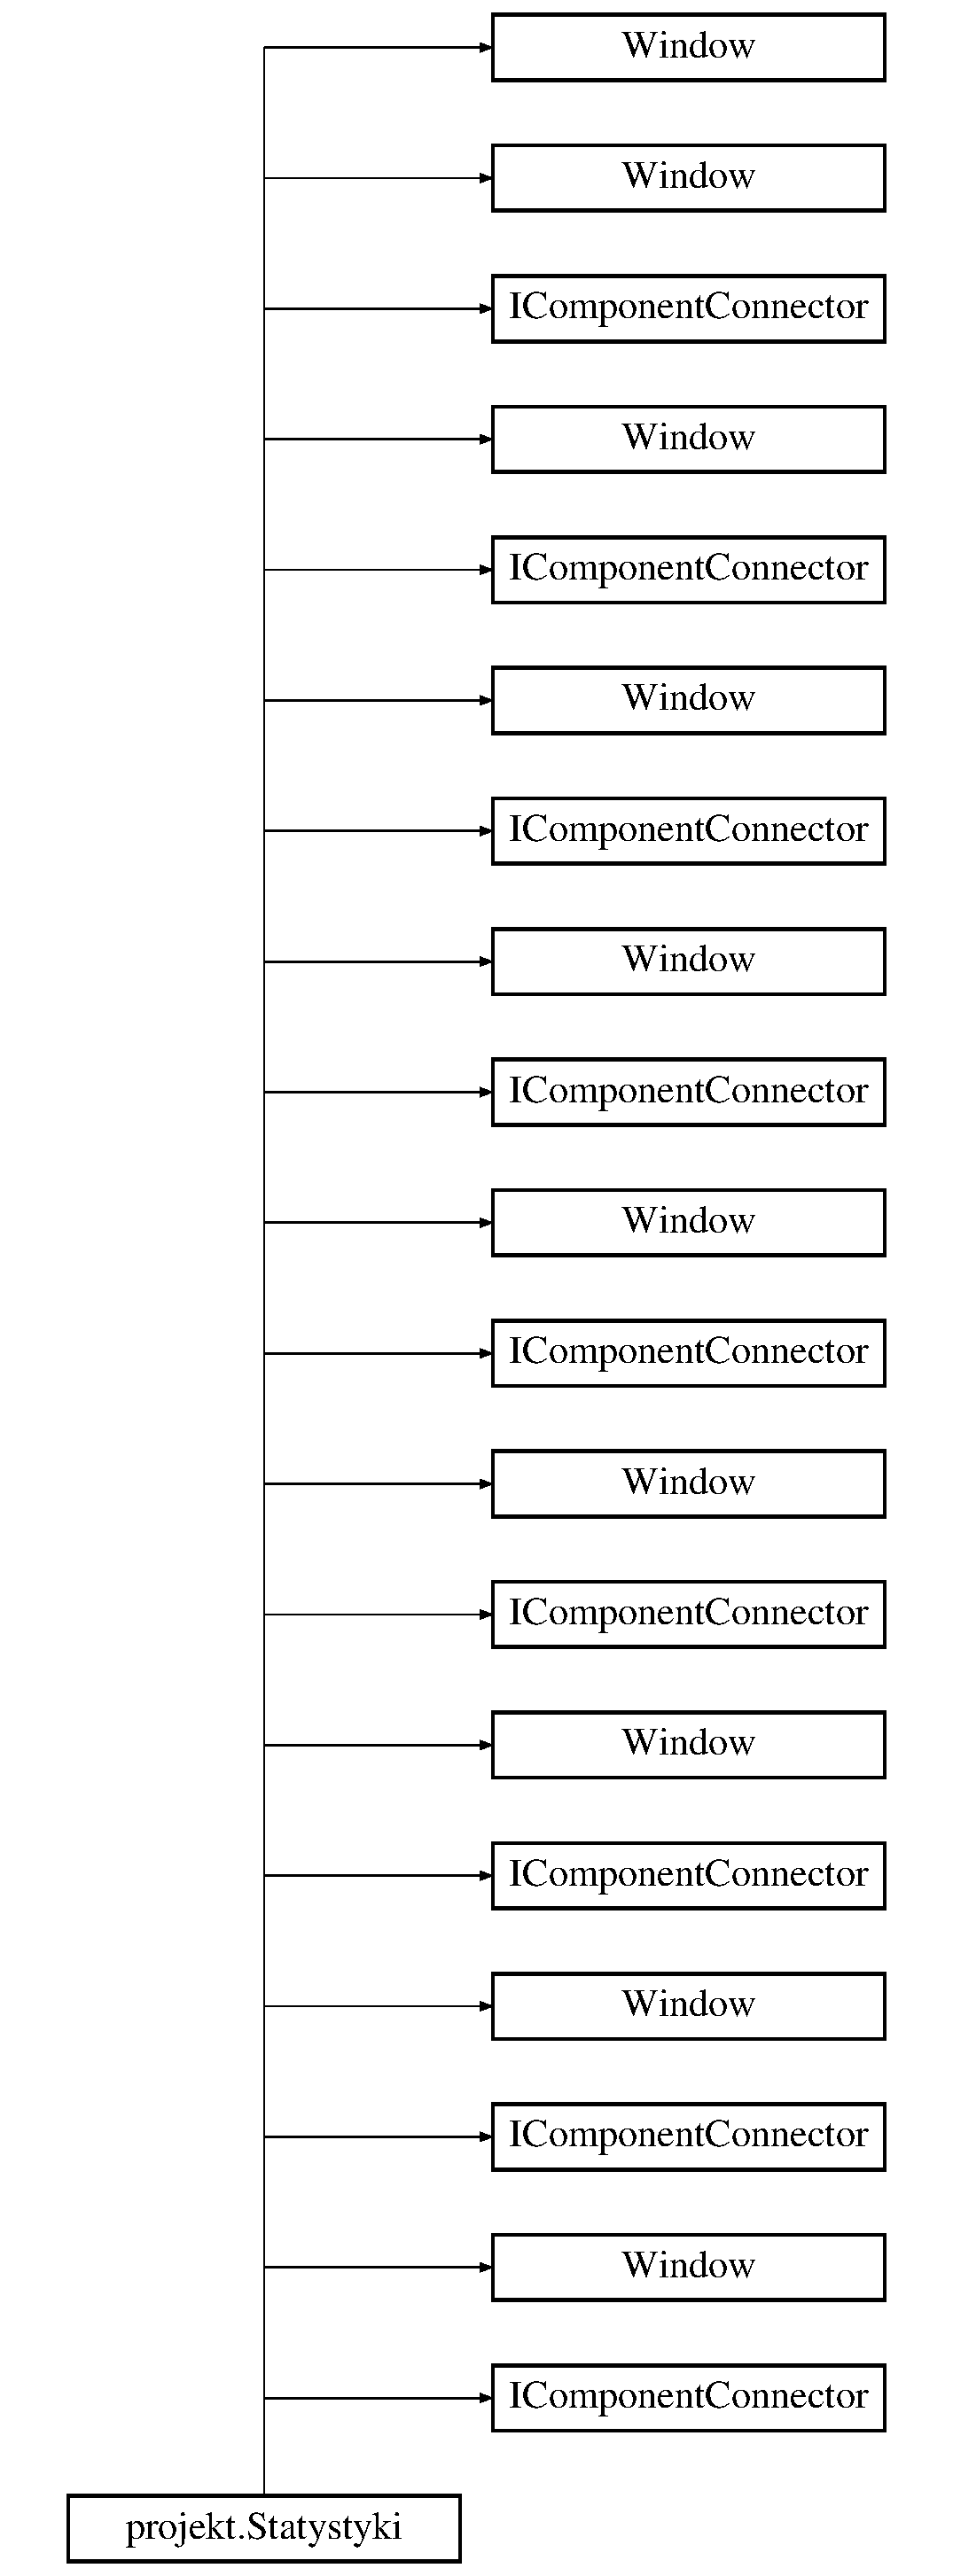
\includegraphics[height=12.000000cm]{classprojekt_1_1_statystyki}
\end{center}
\end{figure}
\subsection*{Public Member Functions}
\begin{DoxyCompactItemize}
\item 
void \mbox{\hyperlink{classprojekt_1_1_statystyki_a6f4801d8176e1c715f5260bf055b0915}{Initialize\+Component}} ()
\begin{DoxyCompactList}\small\item\em Initialize\+Component \end{DoxyCompactList}\item 
void \mbox{\hyperlink{classprojekt_1_1_statystyki_a6f4801d8176e1c715f5260bf055b0915}{Initialize\+Component}} ()
\begin{DoxyCompactList}\small\item\em Initialize\+Component \end{DoxyCompactList}\item 
void \mbox{\hyperlink{classprojekt_1_1_statystyki_a6f4801d8176e1c715f5260bf055b0915}{Initialize\+Component}} ()
\begin{DoxyCompactList}\small\item\em Initialize\+Component \end{DoxyCompactList}\item 
void \mbox{\hyperlink{classprojekt_1_1_statystyki_a6f4801d8176e1c715f5260bf055b0915}{Initialize\+Component}} ()
\begin{DoxyCompactList}\small\item\em Initialize\+Component \end{DoxyCompactList}\item 
void \mbox{\hyperlink{classprojekt_1_1_statystyki_a6f4801d8176e1c715f5260bf055b0915}{Initialize\+Component}} ()
\begin{DoxyCompactList}\small\item\em Initialize\+Component \end{DoxyCompactList}\item 
void \mbox{\hyperlink{classprojekt_1_1_statystyki_a6f4801d8176e1c715f5260bf055b0915}{Initialize\+Component}} ()
\begin{DoxyCompactList}\small\item\em Initialize\+Component \end{DoxyCompactList}\item 
void \mbox{\hyperlink{classprojekt_1_1_statystyki_a6f4801d8176e1c715f5260bf055b0915}{Initialize\+Component}} ()
\begin{DoxyCompactList}\small\item\em Initialize\+Component \end{DoxyCompactList}\item 
void \mbox{\hyperlink{classprojekt_1_1_statystyki_a6f4801d8176e1c715f5260bf055b0915}{Initialize\+Component}} ()
\begin{DoxyCompactList}\small\item\em Initialize\+Component \end{DoxyCompactList}\item 
void \mbox{\hyperlink{classprojekt_1_1_statystyki_a6f4801d8176e1c715f5260bf055b0915}{Initialize\+Component}} ()
\begin{DoxyCompactList}\small\item\em Initialize\+Component \end{DoxyCompactList}\item 
\mbox{\hyperlink{classprojekt_1_1_statystyki_ae90a003d3720200a8ef9b33e6f9f0225}{Statystyki}} ()
\begin{DoxyCompactList}\small\item\em tutaj następuje inicjalizacja bazy danych oraz połączenie poprzez lokalne wskazanie ścieżki pliku \end{DoxyCompactList}\item 
void \mbox{\hyperlink{classprojekt_1_1_statystyki_ad332fb6b7fc8e823ca0f23f3bb9fdc7c}{button\+\_\+\+Click}} (object sender, Routed\+Event\+Args e)
\begin{DoxyCompactList}\small\item\em metoda kliknięcia po kliknięciu w przycisk otwierane jest połączączenie z bazą danych(dokładnie poprzez odwołanie poprzez sql do tabeli przechowującej dane) w tabeli wyświetlane są wyniki wszystkich graczy w razie blędnego połączenia z bazą danych wyświetlany jest komunikat o problemach \end{DoxyCompactList}\end{DoxyCompactItemize}


\subsection{Detailed Description}
\mbox{\hyperlink{classprojekt_1_1_statystyki}{Statystyki}} 

statystyki 

\subsection{Constructor \& Destructor Documentation}
\mbox{\Hypertarget{classprojekt_1_1_statystyki_ae90a003d3720200a8ef9b33e6f9f0225}\label{classprojekt_1_1_statystyki_ae90a003d3720200a8ef9b33e6f9f0225}} 
\index{projekt\+::\+Statystyki@{projekt\+::\+Statystyki}!Statystyki@{Statystyki}}
\index{Statystyki@{Statystyki}!projekt\+::\+Statystyki@{projekt\+::\+Statystyki}}
\subsubsection{\texorpdfstring{Statystyki()}{Statystyki()}}
{\footnotesize\ttfamily projekt.\+Statystyki.\+Statystyki (\begin{DoxyParamCaption}{ }\end{DoxyParamCaption})\hspace{0.3cm}{\ttfamily [inline]}}



tutaj następuje inicjalizacja bazy danych oraz połączenie poprzez lokalne wskazanie ścieżki pliku 



\subsection{Member Function Documentation}
\mbox{\Hypertarget{classprojekt_1_1_statystyki_ad332fb6b7fc8e823ca0f23f3bb9fdc7c}\label{classprojekt_1_1_statystyki_ad332fb6b7fc8e823ca0f23f3bb9fdc7c}} 
\index{projekt\+::\+Statystyki@{projekt\+::\+Statystyki}!button\+\_\+\+Click@{button\+\_\+\+Click}}
\index{button\+\_\+\+Click@{button\+\_\+\+Click}!projekt\+::\+Statystyki@{projekt\+::\+Statystyki}}
\subsubsection{\texorpdfstring{button\+\_\+\+Click()}{button\_Click()}}
{\footnotesize\ttfamily void projekt.\+Statystyki.\+button\+\_\+\+Click (\begin{DoxyParamCaption}\item[{object}]{sender,  }\item[{Routed\+Event\+Args}]{e }\end{DoxyParamCaption})\hspace{0.3cm}{\ttfamily [inline]}}



metoda kliknięcia po kliknięciu w przycisk otwierane jest połączączenie z bazą danych(dokładnie poprzez odwołanie poprzez sql do tabeli przechowującej dane) w tabeli wyświetlane są wyniki wszystkich graczy w razie blędnego połączenia z bazą danych wyświetlany jest komunikat o problemach 

\mbox{\Hypertarget{classprojekt_1_1_statystyki_a6f4801d8176e1c715f5260bf055b0915}\label{classprojekt_1_1_statystyki_a6f4801d8176e1c715f5260bf055b0915}} 
\index{projekt\+::\+Statystyki@{projekt\+::\+Statystyki}!Initialize\+Component@{Initialize\+Component}}
\index{Initialize\+Component@{Initialize\+Component}!projekt\+::\+Statystyki@{projekt\+::\+Statystyki}}
\subsubsection{\texorpdfstring{Initialize\+Component()}{InitializeComponent()}\hspace{0.1cm}{\footnotesize\ttfamily [1/9]}}
{\footnotesize\ttfamily void projekt.\+Statystyki.\+Initialize\+Component (\begin{DoxyParamCaption}{ }\end{DoxyParamCaption})\hspace{0.3cm}{\ttfamily [inline]}}



Initialize\+Component 

\mbox{\Hypertarget{classprojekt_1_1_statystyki_a6f4801d8176e1c715f5260bf055b0915}\label{classprojekt_1_1_statystyki_a6f4801d8176e1c715f5260bf055b0915}} 
\index{projekt\+::\+Statystyki@{projekt\+::\+Statystyki}!Initialize\+Component@{Initialize\+Component}}
\index{Initialize\+Component@{Initialize\+Component}!projekt\+::\+Statystyki@{projekt\+::\+Statystyki}}
\subsubsection{\texorpdfstring{Initialize\+Component()}{InitializeComponent()}\hspace{0.1cm}{\footnotesize\ttfamily [2/9]}}
{\footnotesize\ttfamily void projekt.\+Statystyki.\+Initialize\+Component (\begin{DoxyParamCaption}{ }\end{DoxyParamCaption})\hspace{0.3cm}{\ttfamily [inline]}}



Initialize\+Component 

\mbox{\Hypertarget{classprojekt_1_1_statystyki_a6f4801d8176e1c715f5260bf055b0915}\label{classprojekt_1_1_statystyki_a6f4801d8176e1c715f5260bf055b0915}} 
\index{projekt\+::\+Statystyki@{projekt\+::\+Statystyki}!Initialize\+Component@{Initialize\+Component}}
\index{Initialize\+Component@{Initialize\+Component}!projekt\+::\+Statystyki@{projekt\+::\+Statystyki}}
\subsubsection{\texorpdfstring{Initialize\+Component()}{InitializeComponent()}\hspace{0.1cm}{\footnotesize\ttfamily [3/9]}}
{\footnotesize\ttfamily void projekt.\+Statystyki.\+Initialize\+Component (\begin{DoxyParamCaption}{ }\end{DoxyParamCaption})\hspace{0.3cm}{\ttfamily [inline]}}



Initialize\+Component 

\mbox{\Hypertarget{classprojekt_1_1_statystyki_a6f4801d8176e1c715f5260bf055b0915}\label{classprojekt_1_1_statystyki_a6f4801d8176e1c715f5260bf055b0915}} 
\index{projekt\+::\+Statystyki@{projekt\+::\+Statystyki}!Initialize\+Component@{Initialize\+Component}}
\index{Initialize\+Component@{Initialize\+Component}!projekt\+::\+Statystyki@{projekt\+::\+Statystyki}}
\subsubsection{\texorpdfstring{Initialize\+Component()}{InitializeComponent()}\hspace{0.1cm}{\footnotesize\ttfamily [4/9]}}
{\footnotesize\ttfamily void projekt.\+Statystyki.\+Initialize\+Component (\begin{DoxyParamCaption}{ }\end{DoxyParamCaption})\hspace{0.3cm}{\ttfamily [inline]}}



Initialize\+Component 

\mbox{\Hypertarget{classprojekt_1_1_statystyki_a6f4801d8176e1c715f5260bf055b0915}\label{classprojekt_1_1_statystyki_a6f4801d8176e1c715f5260bf055b0915}} 
\index{projekt\+::\+Statystyki@{projekt\+::\+Statystyki}!Initialize\+Component@{Initialize\+Component}}
\index{Initialize\+Component@{Initialize\+Component}!projekt\+::\+Statystyki@{projekt\+::\+Statystyki}}
\subsubsection{\texorpdfstring{Initialize\+Component()}{InitializeComponent()}\hspace{0.1cm}{\footnotesize\ttfamily [5/9]}}
{\footnotesize\ttfamily void projekt.\+Statystyki.\+Initialize\+Component (\begin{DoxyParamCaption}{ }\end{DoxyParamCaption})\hspace{0.3cm}{\ttfamily [inline]}}



Initialize\+Component 

\mbox{\Hypertarget{classprojekt_1_1_statystyki_a6f4801d8176e1c715f5260bf055b0915}\label{classprojekt_1_1_statystyki_a6f4801d8176e1c715f5260bf055b0915}} 
\index{projekt\+::\+Statystyki@{projekt\+::\+Statystyki}!Initialize\+Component@{Initialize\+Component}}
\index{Initialize\+Component@{Initialize\+Component}!projekt\+::\+Statystyki@{projekt\+::\+Statystyki}}
\subsubsection{\texorpdfstring{Initialize\+Component()}{InitializeComponent()}\hspace{0.1cm}{\footnotesize\ttfamily [6/9]}}
{\footnotesize\ttfamily void projekt.\+Statystyki.\+Initialize\+Component (\begin{DoxyParamCaption}{ }\end{DoxyParamCaption})\hspace{0.3cm}{\ttfamily [inline]}}



Initialize\+Component 

\mbox{\Hypertarget{classprojekt_1_1_statystyki_a6f4801d8176e1c715f5260bf055b0915}\label{classprojekt_1_1_statystyki_a6f4801d8176e1c715f5260bf055b0915}} 
\index{projekt\+::\+Statystyki@{projekt\+::\+Statystyki}!Initialize\+Component@{Initialize\+Component}}
\index{Initialize\+Component@{Initialize\+Component}!projekt\+::\+Statystyki@{projekt\+::\+Statystyki}}
\subsubsection{\texorpdfstring{Initialize\+Component()}{InitializeComponent()}\hspace{0.1cm}{\footnotesize\ttfamily [7/9]}}
{\footnotesize\ttfamily void projekt.\+Statystyki.\+Initialize\+Component (\begin{DoxyParamCaption}{ }\end{DoxyParamCaption})\hspace{0.3cm}{\ttfamily [inline]}}



Initialize\+Component 

\mbox{\Hypertarget{classprojekt_1_1_statystyki_a6f4801d8176e1c715f5260bf055b0915}\label{classprojekt_1_1_statystyki_a6f4801d8176e1c715f5260bf055b0915}} 
\index{projekt\+::\+Statystyki@{projekt\+::\+Statystyki}!Initialize\+Component@{Initialize\+Component}}
\index{Initialize\+Component@{Initialize\+Component}!projekt\+::\+Statystyki@{projekt\+::\+Statystyki}}
\subsubsection{\texorpdfstring{Initialize\+Component()}{InitializeComponent()}\hspace{0.1cm}{\footnotesize\ttfamily [8/9]}}
{\footnotesize\ttfamily void projekt.\+Statystyki.\+Initialize\+Component (\begin{DoxyParamCaption}{ }\end{DoxyParamCaption})\hspace{0.3cm}{\ttfamily [inline]}}



Initialize\+Component 

\mbox{\Hypertarget{classprojekt_1_1_statystyki_a6f4801d8176e1c715f5260bf055b0915}\label{classprojekt_1_1_statystyki_a6f4801d8176e1c715f5260bf055b0915}} 
\index{projekt\+::\+Statystyki@{projekt\+::\+Statystyki}!Initialize\+Component@{Initialize\+Component}}
\index{Initialize\+Component@{Initialize\+Component}!projekt\+::\+Statystyki@{projekt\+::\+Statystyki}}
\subsubsection{\texorpdfstring{Initialize\+Component()}{InitializeComponent()}\hspace{0.1cm}{\footnotesize\ttfamily [9/9]}}
{\footnotesize\ttfamily void projekt.\+Statystyki.\+Initialize\+Component (\begin{DoxyParamCaption}{ }\end{DoxyParamCaption})\hspace{0.3cm}{\ttfamily [inline]}}



Initialize\+Component 



The documentation for this class was generated from the following files\+:\begin{DoxyCompactItemize}
\item 
projekt/obj/\+Debug/\mbox{\hyperlink{_debug_2_statystyki_8g_8cs}{Statystyki.\+g.\+cs}}\item 
projekt/obj/\+Debug/\mbox{\hyperlink{_debug_2_statystyki_8g_8i_8cs}{Statystyki.\+g.\+i.\+cs}}\item 
projekt/\mbox{\hyperlink{_statystyki_8xaml_8cs}{Statystyki.\+xaml.\+cs}}\end{DoxyCompactItemize}

\hypertarget{classprojekt_1_1_tests_1_1_statystyki_tests}{}\section{projekt.\+Tests.\+Statystyki\+Tests Class Reference}
\label{classprojekt_1_1_tests_1_1_statystyki_tests}\index{projekt.\+Tests.\+Statystyki\+Tests@{projekt.\+Tests.\+Statystyki\+Tests}}


 


\subsection*{Public Member Functions}
\begin{DoxyCompactItemize}
\item 
void \mbox{\hyperlink{classprojekt_1_1_tests_1_1_statystyki_tests_a2f1745f7152abbff76600073f94dee62}{Sprawdzenie\+Bazy}} ()
\begin{DoxyCompactList}\small\item\em metoda testująca połączenie z bazą danych, z której będą wyśwoietlane statystyki \end{DoxyCompactList}\end{DoxyCompactItemize}
\subsection*{Public Attributes}
\begin{DoxyCompactItemize}
\item 
Ole\+Db\+Connection \mbox{\hyperlink{classprojekt_1_1_tests_1_1_statystyki_tests_afd97556a71a8fae8cca5c7cdf39dbebe}{connection}} = new Ole\+Db\+Connection()
\end{DoxyCompactItemize}


\subsection{Detailed Description}


klasa testująca \mbox{\hyperlink{classprojekt_1_1_tests_1_1_statystyki_tests}{Statystyki\+Tests}} 

\subsection{Member Function Documentation}
\mbox{\Hypertarget{classprojekt_1_1_tests_1_1_statystyki_tests_a2f1745f7152abbff76600073f94dee62}\label{classprojekt_1_1_tests_1_1_statystyki_tests_a2f1745f7152abbff76600073f94dee62}} 
\index{projekt\+::\+Tests\+::\+Statystyki\+Tests@{projekt\+::\+Tests\+::\+Statystyki\+Tests}!Sprawdzenie\+Bazy@{Sprawdzenie\+Bazy}}
\index{Sprawdzenie\+Bazy@{Sprawdzenie\+Bazy}!projekt\+::\+Tests\+::\+Statystyki\+Tests@{projekt\+::\+Tests\+::\+Statystyki\+Tests}}
\subsubsection{\texorpdfstring{Sprawdzenie\+Bazy()}{SprawdzenieBazy()}}
{\footnotesize\ttfamily void projekt.\+Tests.\+Statystyki\+Tests.\+Sprawdzenie\+Bazy (\begin{DoxyParamCaption}{ }\end{DoxyParamCaption})\hspace{0.3cm}{\ttfamily [inline]}}



metoda testująca połączenie z bazą danych, z której będą wyśwoietlane statystyki 



\subsection{Member Data Documentation}
\mbox{\Hypertarget{classprojekt_1_1_tests_1_1_statystyki_tests_afd97556a71a8fae8cca5c7cdf39dbebe}\label{classprojekt_1_1_tests_1_1_statystyki_tests_afd97556a71a8fae8cca5c7cdf39dbebe}} 
\index{projekt\+::\+Tests\+::\+Statystyki\+Tests@{projekt\+::\+Tests\+::\+Statystyki\+Tests}!connection@{connection}}
\index{connection@{connection}!projekt\+::\+Tests\+::\+Statystyki\+Tests@{projekt\+::\+Tests\+::\+Statystyki\+Tests}}
\subsubsection{\texorpdfstring{connection}{connection}}
{\footnotesize\ttfamily Ole\+Db\+Connection projekt.\+Tests.\+Statystyki\+Tests.\+connection = new Ole\+Db\+Connection()}



The documentation for this class was generated from the following file\+:\begin{DoxyCompactItemize}
\item 
projekt\+Tests2/\mbox{\hyperlink{_statystyki_tests_8cs}{Statystyki\+Tests.\+cs}}\end{DoxyCompactItemize}

\hypertarget{classprojekt_1_1_window1}{}\section{projekt.\+Window1 Class Reference}
\label{classprojekt_1_1_window1}\index{projekt.\+Window1@{projekt.\+Window1}}


\mbox{\hyperlink{classprojekt_1_1_window1}{Window1}}  


Inheritance diagram for projekt.\+Window1\+:\begin{figure}[H]
\begin{center}
\leavevmode
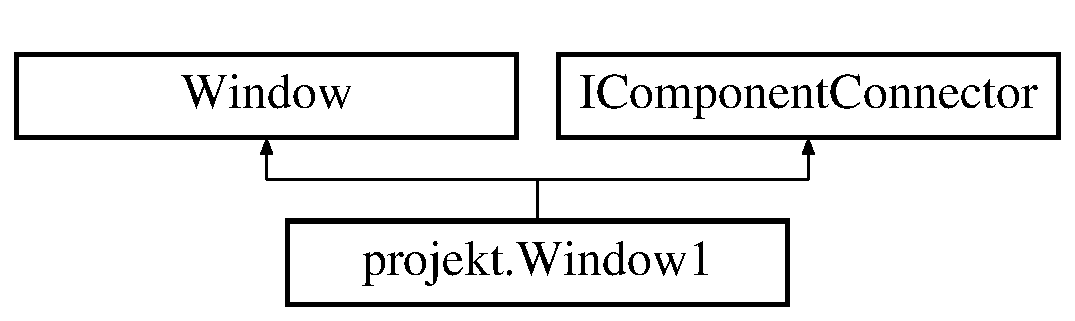
\includegraphics[height=2.000000cm]{classprojekt_1_1_window1}
\end{center}
\end{figure}
\subsection*{Public Member Functions}
\begin{DoxyCompactItemize}
\item 
void \mbox{\hyperlink{classprojekt_1_1_window1_ad2061a2a9cf03f45616950cf16a0784c}{Initialize\+Component}} ()
\begin{DoxyCompactList}\small\item\em Initialize\+Component \end{DoxyCompactList}\end{DoxyCompactItemize}


\subsection{Detailed Description}
\mbox{\hyperlink{classprojekt_1_1_window1}{Window1}} 



\subsection{Member Function Documentation}
\mbox{\Hypertarget{classprojekt_1_1_window1_ad2061a2a9cf03f45616950cf16a0784c}\label{classprojekt_1_1_window1_ad2061a2a9cf03f45616950cf16a0784c}} 
\index{projekt\+::\+Window1@{projekt\+::\+Window1}!Initialize\+Component@{Initialize\+Component}}
\index{Initialize\+Component@{Initialize\+Component}!projekt\+::\+Window1@{projekt\+::\+Window1}}
\subsubsection{\texorpdfstring{Initialize\+Component()}{InitializeComponent()}}
{\footnotesize\ttfamily void projekt.\+Window1.\+Initialize\+Component (\begin{DoxyParamCaption}{ }\end{DoxyParamCaption})\hspace{0.3cm}{\ttfamily [inline]}}



Initialize\+Component 



The documentation for this class was generated from the following file\+:\begin{DoxyCompactItemize}
\item 
projekt/obj/x86/\+Debug/\mbox{\hyperlink{_window1_8g_8i_8cs}{Window1.\+g.\+i.\+cs}}\end{DoxyCompactItemize}

\hypertarget{classprojekt_1_1zmien__haslo}{}\section{projekt.\+zmien\+\_\+haslo Class Reference}
\label{classprojekt_1_1zmien__haslo}\index{projekt.\+zmien\+\_\+haslo@{projekt.\+zmien\+\_\+haslo}}


\mbox{\hyperlink{classprojekt_1_1zmien__haslo}{zmien\+\_\+haslo}}  


Inheritance diagram for projekt.\+zmien\+\_\+haslo\+:\begin{figure}[H]
\begin{center}
\leavevmode
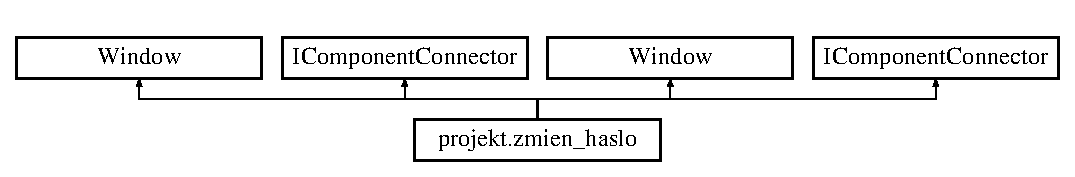
\includegraphics[height=1.931034cm]{classprojekt_1_1zmien__haslo}
\end{center}
\end{figure}
\subsection*{Public Member Functions}
\begin{DoxyCompactItemize}
\item 
void \mbox{\hyperlink{classprojekt_1_1zmien__haslo_a64564a406e807cedb10ae430ccf00577}{Initialize\+Component}} ()
\begin{DoxyCompactList}\small\item\em Initialize\+Component \end{DoxyCompactList}\item 
void \mbox{\hyperlink{classprojekt_1_1zmien__haslo_a64564a406e807cedb10ae430ccf00577}{Initialize\+Component}} ()
\begin{DoxyCompactList}\small\item\em Initialize\+Component \end{DoxyCompactList}\end{DoxyCompactItemize}


\subsection{Detailed Description}
\mbox{\hyperlink{classprojekt_1_1zmien__haslo}{zmien\+\_\+haslo}} 



\subsection{Member Function Documentation}
\mbox{\Hypertarget{classprojekt_1_1zmien__haslo_a64564a406e807cedb10ae430ccf00577}\label{classprojekt_1_1zmien__haslo_a64564a406e807cedb10ae430ccf00577}} 
\index{projekt\+::zmien\+\_\+haslo@{projekt\+::zmien\+\_\+haslo}!Initialize\+Component@{Initialize\+Component}}
\index{Initialize\+Component@{Initialize\+Component}!projekt\+::zmien\+\_\+haslo@{projekt\+::zmien\+\_\+haslo}}
\subsubsection{\texorpdfstring{Initialize\+Component()}{InitializeComponent()}\hspace{0.1cm}{\footnotesize\ttfamily [1/2]}}
{\footnotesize\ttfamily void projekt.\+zmien\+\_\+haslo.\+Initialize\+Component (\begin{DoxyParamCaption}{ }\end{DoxyParamCaption})\hspace{0.3cm}{\ttfamily [inline]}}



Initialize\+Component 

\mbox{\Hypertarget{classprojekt_1_1zmien__haslo_a64564a406e807cedb10ae430ccf00577}\label{classprojekt_1_1zmien__haslo_a64564a406e807cedb10ae430ccf00577}} 
\index{projekt\+::zmien\+\_\+haslo@{projekt\+::zmien\+\_\+haslo}!Initialize\+Component@{Initialize\+Component}}
\index{Initialize\+Component@{Initialize\+Component}!projekt\+::zmien\+\_\+haslo@{projekt\+::zmien\+\_\+haslo}}
\subsubsection{\texorpdfstring{Initialize\+Component()}{InitializeComponent()}\hspace{0.1cm}{\footnotesize\ttfamily [2/2]}}
{\footnotesize\ttfamily void projekt.\+zmien\+\_\+haslo.\+Initialize\+Component (\begin{DoxyParamCaption}{ }\end{DoxyParamCaption})\hspace{0.3cm}{\ttfamily [inline]}}



Initialize\+Component 



The documentation for this class was generated from the following files\+:\begin{DoxyCompactItemize}
\item 
projekt/obj/x86/\+Debug/\mbox{\hyperlink{zmien__haslo_8g_8cs}{zmien\+\_\+haslo.\+g.\+cs}}\item 
projekt/obj/x86/\+Debug/\mbox{\hyperlink{zmien__haslo_8g_8i_8cs}{zmien\+\_\+haslo.\+g.\+i.\+cs}}\end{DoxyCompactItemize}

\chapter{File Documentation}
\input{_app_8xaml_8cs}
\input{_data_set1_8_designer_8cs}
\section{projekt/konto\+\_\+u.xaml.\+cs File Reference}
\label{konto__u_8xaml_8cs}\index{projekt/konto\+\_\+u.\+xaml.\+cs@{projekt/konto\+\_\+u.\+xaml.\+cs}}
\subsection*{Classes}
\begin{DoxyCompactItemize}
\item 
class \textbf{ projekt.\+konto\+\_\+u}
\begin{DoxyCompactList}\small\item\em Interaction logic for konto\+\_\+u.\+xaml \end{DoxyCompactList}\end{DoxyCompactItemize}
\subsection*{Namespaces}
\begin{DoxyCompactItemize}
\item 
namespace \textbf{ projekt}
\end{DoxyCompactItemize}

\input{_debug_2_app_8g_8cs}
\input{x64_2_debug_2_app_8g_8cs}
\input{x86_2_debug_2_app_8g_8cs}
\input{x86_2_release_2_app_8g_8cs}
\input{_debug_2_app_8g_8i_8cs}
\input{x64_2_debug_2_app_8g_8i_8cs}
\input{x64_2_release_2_app_8g_8i_8cs}
\input{x86_2_debug_2_app_8g_8i_8cs}
\input{x86_2_release_2_app_8g_8i_8cs}
\input{_debug_2konto_8g_8i_8cs}
\input{x86_2_debug_2konto_8g_8i_8cs}
\input{_debug_2konto__u_8g_8cs}
\input{x64_2_debug_2konto__u_8g_8cs}
\input{x86_2_debug_2konto__u_8g_8cs}
\input{x86_2_release_2konto__u_8g_8cs}
\input{_debug_2konto__u_8g_8i_8cs}
\input{x64_2_debug_2konto__u_8g_8i_8cs}
\input{x64_2_release_2konto__u_8g_8i_8cs}
\input{x86_2_debug_2konto__u_8g_8i_8cs}
\input{x86_2_release_2konto__u_8g_8i_8cs}
\input{_debug_2panel1_8g_8cs}
\input{x64_2_debug_2panel1_8g_8cs}
\input{x86_2_debug_2panel1_8g_8cs}
\input{x86_2_release_2panel1_8g_8cs}
\input{_debug_2panel1_8g_8i_8cs}
\input{x64_2_debug_2panel1_8g_8i_8cs}
\input{x64_2_release_2panel1_8g_8i_8cs}
\input{x86_2_debug_2panel1_8g_8i_8cs}
\input{x86_2_release_2panel1_8g_8i_8cs}
\input{_debug_2panel__log_8g_8cs}
\input{x64_2_debug_2panel__log_8g_8cs}
\input{x86_2_debug_2panel__log_8g_8cs}
\input{x86_2_release_2panel__log_8g_8cs}
\input{_debug_2panel__log_8g_8i_8cs}
\input{x64_2_debug_2panel__log_8g_8i_8cs}
\input{x64_2_release_2panel__log_8g_8i_8cs}
\input{x86_2_debug_2panel__log_8g_8i_8cs}
\input{x86_2_release_2panel__log_8g_8i_8cs}
\input{_debug_2panel__rej_8g_8cs}
\input{x64_2_debug_2panel__rej_8g_8cs}
\input{x86_2_debug_2panel__rej_8g_8cs}
\input{x86_2_release_2panel__rej_8g_8cs}
\input{_debug_2panel__rej_8g_8i_8cs}
\input{x64_2_debug_2panel__rej_8g_8i_8cs}
\input{x64_2_release_2panel__rej_8g_8i_8cs}
\input{x86_2_debug_2panel__rej_8g_8i_8cs}
\input{x86_2_release_2panel__rej_8g_8i_8cs}
\input{_debug_2pole__gry_8g_8cs}
\input{x64_2_debug_2pole__gry_8g_8cs}
\input{x86_2_debug_2pole__gry_8g_8cs}
\input{x86_2_release_2pole__gry_8g_8cs}
\input{_debug_2pole__gry_8g_8i_8cs}
\input{x64_2_debug_2pole__gry_8g_8i_8cs}
\input{x64_2_release_2pole__gry_8g_8i_8cs}
\input{x86_2_debug_2pole__gry_8g_8i_8cs}
\input{x86_2_release_2pole__gry_8g_8i_8cs}
\input{_debug_2_statystyki_8g_8cs}
\input{x64_2_debug_2_statystyki_8g_8cs}
\input{x86_2_debug_2_statystyki_8g_8cs}
\input{x86_2_release_2_statystyki_8g_8cs}
\input{_debug_2_statystyki_8g_8i_8cs}
\input{x64_2_debug_2_statystyki_8g_8i_8cs}
\input{x64_2_release_2_statystyki_8g_8i_8cs}
\input{x86_2_debug_2_statystyki_8g_8i_8cs}
\input{x86_2_release_2_statystyki_8g_8i_8cs}
\input{obj_2_debug_2_temporary_generated_file__036_c0_b5_b-1481-4323-8_d20-8_f5_a_d_c_b23_d92_8cs}
\input{obj_2x64_2_debug_2_temporary_generated_file__036_c0_b5_b-1481-4323-8_d20-8_f5_a_d_c_b23_d92_8cs}
\input{obj_2x64_2_release_2_temporary_generated_file__036_c0_b5_b-1481-4323-8_d20-8_f5_a_d_c_b23_d92_8cs}
\input{obj_2x86_2_debug_2_temporary_generated_file__036_c0_b5_b-1481-4323-8_d20-8_f5_a_d_c_b23_d92_8cs}
\input{obj_2x86_2_release_2_temporary_generated_file__036_c0_b5_b-1481-4323-8_d20-8_f5_a_d_c_b23_d92_8cs}
\input{ests2_2obj_2_debug_2_temporary_generated_file__036_c0_b5_b-1481-4323-8_d20-8_f5_a_d_c_b23_d92_8cs}
\input{obj_2_debug_2_temporary_generated_file__5937a670-0e60-4077-877b-f7221da3dda1_8cs}
\input{obj_2x64_2_debug_2_temporary_generated_file__5937a670-0e60-4077-877b-f7221da3dda1_8cs}
\input{obj_2x64_2_release_2_temporary_generated_file__5937a670-0e60-4077-877b-f7221da3dda1_8cs}
\input{obj_2x86_2_debug_2_temporary_generated_file__5937a670-0e60-4077-877b-f7221da3dda1_8cs}
\input{obj_2x86_2_release_2_temporary_generated_file__5937a670-0e60-4077-877b-f7221da3dda1_8cs}
\input{ests2_2obj_2_debug_2_temporary_generated_file__5937a670-0e60-4077-877b-f7221da3dda1_8cs}
\input{obj_2_debug_2_temporary_generated_file___e7_a71_f73-0_f8_d-4_b9_b-_b56_e-8_e70_b10_b_c5_d3_8cs}
\input{obj_2x64_2_debug_2_temporary_generated_file___e7_a71_f73-0_f8_d-4_b9_b-_b56_e-8_e70_b10_b_c5_d3_8cs}
\input{obj_2x64_2_release_2_temporary_generated_file___e7_a71_f73-0_f8_d-4_b9_b-_b56_e-8_e70_b10_b_c5_d3_8cs}
\input{obj_2x86_2_debug_2_temporary_generated_file___e7_a71_f73-0_f8_d-4_b9_b-_b56_e-8_e70_b10_b_c5_d3_8cs}
\input{obj_2x86_2_release_2_temporary_generated_file___e7_a71_f73-0_f8_d-4_b9_b-_b56_e-8_e70_b10_b_c5_d3_8cs}
\input{ests2_2obj_2_debug_2_temporary_generated_file___e7_a71_f73-0_f8_d-4_b9_b-_b56_e-8_e70_b10_b_c5_d3_8cs}
\input{projekt___content_8g_8i_8cs}
\input{_window1_8g_8i_8cs}
\section{projekt/obj/x86/\+Debug/zmien\+\_\+haslo.g.\+cs File Reference}
\label{zmien__haslo_8g_8cs}\index{projekt/obj/x86/\+Debug/zmien\+\_\+haslo.\+g.\+cs@{projekt/obj/x86/\+Debug/zmien\+\_\+haslo.\+g.\+cs}}
\subsection*{Classes}
\begin{DoxyCompactItemize}
\item 
class \textbf{ projekt.\+zmien\+\_\+haslo}
\begin{DoxyCompactList}\small\item\em \doxyref{zmien\+\_\+haslo}{p.}{classprojekt_1_1zmien__haslo} \end{DoxyCompactList}\end{DoxyCompactItemize}
\subsection*{Namespaces}
\begin{DoxyCompactItemize}
\item 
namespace \textbf{ projekt}
\end{DoxyCompactItemize}

\section{projekt/obj/x86/\+Debug/zmien\+\_\+haslo.g.\+i.\+cs File Reference}
\label{zmien__haslo_8g_8i_8cs}\index{projekt/obj/x86/\+Debug/zmien\+\_\+haslo.\+g.\+i.\+cs@{projekt/obj/x86/\+Debug/zmien\+\_\+haslo.\+g.\+i.\+cs}}
\subsection*{Classes}
\begin{DoxyCompactItemize}
\item 
class \textbf{ projekt.\+zmien\+\_\+haslo}
\begin{DoxyCompactList}\small\item\em \doxyref{zmien\+\_\+haslo}{p.}{classprojekt_1_1zmien__haslo} \end{DoxyCompactList}\end{DoxyCompactItemize}
\subsection*{Namespaces}
\begin{DoxyCompactItemize}
\item 
namespace \textbf{ projekt}
\end{DoxyCompactItemize}

\hypertarget{panel1_8xaml_8cs}{}\section{projekt/panel1.xaml.\+cs File Reference}
\label{panel1_8xaml_8cs}\index{projekt/panel1.\+xaml.\+cs@{projekt/panel1.\+xaml.\+cs}}
\subsection*{Classes}
\begin{DoxyCompactItemize}
\item 
class \mbox{\hyperlink{classprojekt_1_1panel1}{projekt.\+panel1}}
\begin{DoxyCompactList}\small\item\em \mbox{\hyperlink{classprojekt_1_1panel1}{panel1}} \end{DoxyCompactList}\end{DoxyCompactItemize}
\subsection*{Namespaces}
\begin{DoxyCompactItemize}
\item 
namespace \mbox{\hyperlink{namespaceprojekt}{projekt}}
\end{DoxyCompactItemize}

\section{projekt/panel\+\_\+log.xaml.\+cs File Reference}
\label{panel__log_8xaml_8cs}\index{projekt/panel\+\_\+log.\+xaml.\+cs@{projekt/panel\+\_\+log.\+xaml.\+cs}}
\subsection*{Classes}
\begin{DoxyCompactItemize}
\item 
class \textbf{ projekt.\+panel\+\_\+log}
\begin{DoxyCompactList}\small\item\em \doxyref{panel\+\_\+log}{p.}{classprojekt_1_1panel__log} \end{DoxyCompactList}\end{DoxyCompactItemize}
\subsection*{Namespaces}
\begin{DoxyCompactItemize}
\item 
namespace \textbf{ projekt}
\end{DoxyCompactItemize}

\hypertarget{panel__rej_8xaml_8cs}{}\section{projekt/panel\+\_\+rej.xaml.\+cs File Reference}
\label{panel__rej_8xaml_8cs}\index{projekt/panel\+\_\+rej.\+xaml.\+cs@{projekt/panel\+\_\+rej.\+xaml.\+cs}}
\subsection*{Classes}
\begin{DoxyCompactItemize}
\item 
class \mbox{\hyperlink{classprojekt_1_1panel__rej}{projekt.\+panel\+\_\+rej}}
\begin{DoxyCompactList}\small\item\em \mbox{\hyperlink{classprojekt_1_1panel__rej}{panel\+\_\+rej}} \end{DoxyCompactList}\end{DoxyCompactItemize}
\subsection*{Namespaces}
\begin{DoxyCompactItemize}
\item 
namespace \mbox{\hyperlink{namespaceprojekt}{projekt}}
\end{DoxyCompactItemize}

\section{projekt/pole\+\_\+gry.xaml.\+cs File Reference}
\label{pole__gry_8xaml_8cs}\index{projekt/pole\+\_\+gry.\+xaml.\+cs@{projekt/pole\+\_\+gry.\+xaml.\+cs}}
\subsection*{Classes}
\begin{DoxyCompactItemize}
\item 
class \textbf{ projekt.\+pole\+\_\+gry}
\begin{DoxyCompactList}\small\item\em \doxyref{pole\+\_\+gry}{p.}{classprojekt_1_1pole__gry} \end{DoxyCompactList}\end{DoxyCompactItemize}
\subsection*{Namespaces}
\begin{DoxyCompactItemize}
\item 
namespace \textbf{ projekt}
\end{DoxyCompactItemize}

\input{_properties_2_assembly_info_8cs}
\input{ests2_2_properties_2_assembly_info_8cs}
\input{_resources_8_designer_8cs}
\input{_settings_8_designer_8cs}
\input{_statystyki_8xaml_8cs}
\input{panel__log_tests_8cs}
\input{panel__rej_tests_8cs}
\input{pole__gry_tests_8cs}
\input{_statystyki_tests_8cs}
%--- End generated contents ---

% Index
\backmatter
\newpage
\phantomsection
\clearemptydoublepage
\addcontentsline{toc}{chapter}{Index}
\printindex

\end{document}
